\documentclass[a4paper,13.5pt]{extreport} 

% --- CÁC GÓI LỆNH CẦN THIẾT ---
\usepackage[utf8]{inputenc}
\usepackage[T5]{fontenc}
\usepackage[vietnamese]{babel}
\usepackage{mathptmx} % Font Times New Roman
\usepackage{geometry}
\usepackage{amsmath}
\usepackage{tikz} 
\usepackage{xurl}
\usepackage{indentfirst} % Ép thụt lề đoạn đầu tiên sau tiêu đề
\setlength{\parskip}{3pt} % Thêm một chút khoảng cách siêu nhỏ giữa các đoạn cho thoáng
\usepackage{enumitem}
\usepackage{listings} 
\usepackage{float}
\usetikzlibrary{shapes.geometric, fit, positioning, arrows.meta}
\geometry{
    a4paper,
    left=30mm,   % Lề trái 3.0 cm
    right=20mm,  % Lề phải 2.0 cm
    top=25mm,    % Lề trên 2.5 cm
    bottom=25mm, % Lề dưới 2.5 cm
}
\usepackage{graphicx} 
\usetikzlibrary{calc}
\usepackage{tabularx} 
\usepackage{multirow}
\usepackage{array} 
\usepackage{setspace} 
\usepackage{titlesec} 

% --- GÓI LỆNH TẠO LINK LIÊN KẾT (ĐẶT Ở CUỐI CÙNG) ---
\usepackage{hyperref}
\hypersetup{
    colorlinks=true,     
    linkcolor=black,     
    urlcolor=blue,       
    citecolor=black,     
    pdftitle={Báo cáo Bài tập lớn MIS}, 
    pdfauthor={Nhóm sinh viên}          
}

% --- TẠO KIỂU CỘT MỚI CHO BẢNG ---
\newcolumntype{C}[1]{>{\centering\arraybackslash}p{#1}}
\newcolumntype{M}[1]{>{\centering\arraybackslash}m{#1}}

% --- CẤU HÌNH ĐỊNH DẠNG TIÊU ĐỀ CHƯƠNG ---
\titleformat{\chapter}[block]
  {\normalfont\bfseries\Large\centering}{CHƯƠNG \thechapter:\ }{0pt}{\Large\MakeUppercase}
\titleformat{name=\chapter,numberless}[block]
  {\normalfont\bfseries\Large\centering}{}{0pt}{\Large\MakeUppercase}
\titlespacing*{\chapter}{0pt}{10pt}{20pt}

% Format Section & Subsection
\titleformat{\section}[block]
  {\normalfont\bfseries\large}{\thesection.\ }{0pt}{}
\titleformat{\subsection}[block]
  {\normalfont\bfseries\normalsize}{\thesubsection.\ }{0pt}{}

\begin{document}
\setstretch{1.3} 

% ===================================================
% 1. TRANG BÌA NGOÀI
% ===================================================
\begin{titlepage}
\begin{tikzpicture}[remember picture, overlay]
  \draw[line width = 1.5pt] ($(current page.north west) + (2cm,-2cm)$) rectangle ($(current page.south east) + (-1.5cm,2cm)$);
  \draw[line width = 0.5pt] ($(current page.north west) + (2.1cm,-2.1cm)$) rectangle ($(current page.south east) + (-1.6cm,2.1cm)$);
\end{tikzpicture}

\begin{center}
    \textbf{\large BỘ GIÁO DỤC VÀ ĐÀO TẠO}\\
    \textbf{\large TRƯỜNG ĐẠI HỌC ĐẠI NAM}\\
    \vspace{0.6cm} 
    
    
\includegraphics[width=3.5cm]{logo_dai_nam.jpg} \\
    \vspace{0.6cm} 
    
    \textbf{\Huge BÀI TẬP LỚN}\\
    \vspace{0.5cm}
    
    \textbf{\large TÊN HỌC PHẦN}\\
    \textbf{\large HỆ THỐNG THÔNG TIN QUẢN LÝ}\\
    \vspace{0.6cm}
    
    \textbf{\large ĐỀ TÀI: HỆ THỐNG QUẢN LÝ DỰ ÁN VÀ CHẤM CÔNG KPI}\\
    \textbf{\large (PROJECT \& TASK MANAGEMENT)}\\
\end{center}

\vspace{1.0cm} 
\begin{center}
\begin{minipage}{10.5cm} 
    \textbf{Giáo viên hướng dẫn: ThS. Đỗ Quang Thơ}\\[0.2cm]
    \textbf{Sinh viên thực hiện: Nhóm 8}
    
    \vspace{0.3cm}
    \renewcommand{\arraystretch}{1.5}
    \begin{tabular}{|c|C{2.5cm}|C{4cm}|C{2cm}|}
    \hline
    \textbf{STT} & \textbf{Mã SV} & \textbf{Họ và tên} & \textbf{Lớp} \\
    \hline
    1 &1871040025 &Nguyễn Xong Phi &KHMT 18-01 \\
    \hline
    2 &1871040012  &Lê Quốc Duy&KHMT 18-01  \\
    \hline
    3 &1871040026 &Đoàn Đức Phúc &KHMT 18-01 \\
    \hline
    \end{tabular}
\end{minipage}
\end{center}

\vfill
\begin{center}
    \textbf{Hà Nội, năm 2026}
\end{center}
\end{titlepage}

% ===================================================
% 2. TRANG BÌA TRONG (BÌA CHẤM ĐIỂM)
% ===================================================
\begin{titlepage}
\begin{tikzpicture}[remember picture, overlay]
  \draw[line width = 1.5pt] ($(current page.north west) + (2cm,-2cm)$) rectangle ($(current page.south east) + (-1.5cm,2cm)$);
  \draw[line width = 0.5pt] ($(current page.north west) + (2.1cm,-2.1cm)$) rectangle ($(current page.south east) + (-1.6cm,2.1cm)$);
\end{tikzpicture}

\begin{center}
    \textbf{\large BỘ GIÁO DỤC VÀ ĐÀO TẠO}\\
    \textbf{\large TRƯỜNG ĐẠI HỌC ĐẠI NAM}\\
    \vspace{0.6cm}
    
    
\includegraphics[width=3.5cm]{logo_dai_nam.jpg} \\
    \vspace{0.6cm}
    
    \textbf{\Huge BÀI TẬP LỚN}\\
    \vspace{0.5cm}
    
    \textbf{\large TÊN HỌC PHẦN}\\
    \textbf{\large HỆ THỐNG THÔNG TIN QUẢN LÝ}\\
    \vspace{0.6cm}
    
    \textbf{\large ĐỀ TÀI: HỆ THỐNG QUẢN LÝ DỰ ÁN VÀ CHẤM CÔNG KPI}\\
    \textbf{\large (PROJECT \& TASK MANAGEMENT)}\\
\end{center}

\vspace{1.0cm}
\begin{center}
\renewcommand{\arraystretch}{1.6}
\begin{tabular}{|c|M{2.5cm}|M{4cm}|C{2cm}|C{2cm}|}
\hline
\multirow{2}{*}{\textbf{STT}} & \multirow{2}{=}{\centering \textbf{Mã Sinh Viên}} & \multirow{2}{=}{\centering \textbf{Họ và Tên}} & \multicolumn{2}{c|}{\textbf{Điểm}} \\ 
\cline{4-5}
 & & & \textbf{Bằng Số} & \textbf{Bằng Chữ} \\
\hline
1 &1871040025&Nguyễn Xong Phi & & \\
\hline
2 &1871040012 &Lê Quốc Duy & & \\
\hline
3 &1871040026 &Đoàn Đức Phúc & & \\
\hline
\end{tabular}
\end{center}

\vspace{1.2cm}
\begin{center}
\begin{minipage}{0.45\textwidth}
\centering
\textbf{CÁN BỘ CHẤM THI 1}
\end{minipage}%
\begin{minipage}{0.45\textwidth}
\centering
\textbf{CÁN BỘ CHẤM THI 2}
\end{minipage}
\end{center}

\vfill
\begin{center}
    \textbf{Hà Nội, năm 2026}
\end{center}
\end{titlepage}

% ===================================================
% 3. LỜI CẢM ƠN
% ===================================================
\chapter*{LỜI CẢM ƠN}
\addcontentsline{toc}{chapter}{LỜI CẢM ƠN}

\vspace{0.5cm} 

Lời đầu tiên, chúng em xin chân thành cảm ơn Ban Giám hiệu cùng các thầy cô giáo thuộc Khoa Công nghệ thông tin – Trường Đại học Đại Nam đã tạo điều kiện học tập tốt nhất để chúng em có nền tảng kiến thức vững chắc vững bước vào chuyên ngành.

Đặc biệt, chúng em xin bày tỏ lòng biết ơn sâu sắc nhất đến \textbf{ThS. Đỗ Quang Thơ} – giảng viên hướng dẫn trực tiếp học phần Hệ thống thông tin quản lý. Trong suốt quá trình nghiên cứu và phát triển đề tài \textit{“Hệ thống quản lý dự án và chấm công KPI (Project \& Task Management)”}, thầy đã luôn dành thời gian tận tình chỉ bảo, định hướng tư duy phân tích hệ thống và đưa ra những lời khuyên chuyên môn vô cùng quý báu giúp chúng em tháo gỡ nhiều nút thắt kỹ thuật khó. Sự đồng hành của thầy chính là động lực lớn nhất để nhóm có thể hoàn thiện sản phẩm báo cáo này.

Mặc dù đã đầu tư nhiều thời gian và tâm huyết, song do giới hạn về mặt kinh nghiệm thực tiễn nên bài tập lớn của chúng em chắc chắn không tránh khỏi những thiếu sót ngoài ý muốn. Nhóm chúng em rất mong tiếp tục nhận được những lời phê bình, nhận xét và ý kiến đóng góp từ thầy để hệ thống được hoàn thiện tối ưu hơn trong tương lai.

Chúng em xin chân thành cảm ơn thầy!

\vspace{1.5cm}
\begin{flushright}
    \begin{minipage}{6.5cm} 
        \centering 
        \textit{Hà Nội, năm 2026}\\[0.2cm]
        \textbf{Nhóm sinh viên thực hiện}\\[0.1cm]
    \end{minipage}
\end{flushright}

\newpage

% ===================================================
% 4. DANH MỤC VIẾT TẮT
% ===================================================
\chapter*{DANH MỤC VIẾT TẮT}
\addcontentsline{toc}{chapter}{DANH MỤC VIẾT TẮT}

\vspace{0.5cm}
\renewcommand{\arraystretch}{1.5}
\begin{table}[H]
    \centering
    \begin{tabularx}{\textwidth}{|C{3.5cm}|X|}
    \hline
    \textbf{Từ viết tắt} & \multicolumn{1}{c|}{\textbf{Lý giải từ viết tắt}} \\
    \hline
    \textbf{3NF} & Dạng chuẩn 3 (Third Normal Form) \\
    \hline
    \textbf{CRUD} & Các thao tác cơ bản với cơ sở dữ liệu: Tạo, Đọc, Cập nhật, Xóa (Create, Read, Update, Delete) \\
    \hline
    \textbf{ERD} & Sơ đồ thực thể liên kết (Entity-Relationship Diagram) \\
    \hline
    \textbf{HRM} & Hệ thống Quản trị Nguồn nhân lực (Human Resource Management) \\
    \hline
    \textbf{KPI} & Chỉ số đánh giá thực hiện công việc (Key Performance Indicator) \\
    \hline
    \textbf{MIS} & Hệ thống thông tin quản lý (Management Information System) \\
    \hline
    \textbf{MSSQL} & Hệ quản trị cơ sở dữ liệu Microsoft SQL Server \\
    \hline
    \textbf{SMART} & Tiêu chí thiết lập mục tiêu (Cụ thể - Đo lường được - Khả thi - Thực tế - Có thời hạn) \\
    \hline
    \textbf{WBS} & Cấu trúc phân rã công việc (Work Breakdown Structure) \\
    \hline
    \end{tabularx}
\end{table}

\newpage

% ===================================================
% 5. DANH MỤC HÌNH ẢNH, BẢNG BIỂU
% ===================================================
\renewcommand{\listfigurename}{DANH MỤC HÌNH ẢNH}
\listoffigures
\addcontentsline{toc}{chapter}{DANH MỤC HÌNH ẢNH}

\newpage

% ==================================================
% DANH MỤC BẢNG BIỂU
% ==================================================
\renewcommand{\listtablename}{DANH MỤC BẢNG BIỂU}
\listoftables
\addcontentsline{toc}{chapter}{DANH MỤC BẢNG BIỂU}

\newpage

% ===================================================
% 6. MỤC LỤC
% ===================================================
\renewcommand{\contentsname}{MỤC LỤC}
\tableofcontents
\newpage

% ===================================================
% NỘI DUNG BÁO CÁO 
% ===================================================

% --- LỜI MỞ ĐẦU ---
\chapter*{LỜI MỞ ĐẦU}
\addcontentsline{toc}{chapter}{LỜI MỞ ĐẦU}

Trong kỷ nguyên chuyển đổi số hiện nay, quản lý dự án và tối ưu hóa nguồn nhân lực không chỉ là yêu cầu nội bộ mà đã trở thành yếu tố sống còn quyết định năng lực cạnh tranh của mọi doanh nghiệp. Đặc biệt trong lĩnh vực công nghệ thông tin, nơi mà các dự án phần mềm thường có độ phức tạp kỹ thuật cao, yêu cầu sự phối hợp liên tục (Agile/Scrum) và vòng đời thay đổi linh hoạt, việc kiểm soát chặt chẽ tiến độ cũng như đánh giá chính xác hiệu suất làm việc của từng cá nhân lại càng trở nên cấp thiết.

Thực tiễn cho thấy, nhiều tổ chức và doanh nghiệp hiện nay vẫn đang phụ thuộc vào các phương thức quản trị truyền thống, sử dụng các công cụ rời rạc như bảng tính Excel, email hay các ứng dụng nhắn tin tức thời. Mô hình này không những tạo ra "độ trễ" trong giao tiếp mà còn dẫn đến tình trạng "mù thông tin" đối với cấp quản lý. Hậu quả tất yếu là rủi ro trễ hạn (miss deadline) không được cảnh báo sớm, tình trạng phân bổ nguồn lực bất hợp lý (người quá tải, người thiếu việc) thường xuyên xảy ra. Đáng lo ngại hơn, công tác đánh giá hiệu suất (KPI) vào mỗi cuối tháng thường tốn rất nhiều thời gian tổng hợp thủ công, dễ bị chi phối bởi góc nhìn cảm tính, dẫn đến sự thiếu minh bạch và làm giảm động lực cống hiến của người lao động.

Xuất phát từ nhu cầu giải quyết triệt để những điểm nghẽn nghiệp vụ nêu trên, đề tài/dự án \textbf{"Xây dựng Hệ thống thông tin quản lý (MIS) tiến độ công việc và đánh giá KPI tự động"} đã được nghiên cứu và thực hiện. 

Mục tiêu cốt lõi của hệ thống là kiến tạo một không gian làm việc số tập trung (Centralized Digital Workspace). Bằng việc ứng dụng triết lý thiết kế lấy người dùng làm trung tâm (User-Centered Design) và kiến trúc phần mềm hiện đại, dự án đã triển khai thành công mô hình Single Page Application (SPA) bằng ReactJS kết hợp cùng hệ thống Backend mạnh mẽ viết bằng C\# .NET Core và cơ sở dữ liệu Microsoft SQL Server. Sự kết hợp này mang lại trải nghiệm tương tác mượt mà qua các bảng Kanban trực quan, số hóa toàn diện quy trình giao việc (WBS) và báo cáo giờ làm (Log-time). Hơn thế nữa, hệ thống tự hào tích hợp "Động cơ tính toán KPI" chạy ngầm tự động (thông qua Hangfire), giúp lượng hóa 100\% hiệu suất nhân sự dựa trên dữ liệu thực tế, đảm bảo tính công bằng tuyệt đối và giải phóng hoàn toàn gánh nặng hành chính cho khối Quản trị Nhân sự (HR).

Nội dung của báo cáo được tổ chức logic, đi từ tổng quan đến chi tiết kỹ thuật, bao gồm 5 chương chính:
\begin{itemize}
    \item \textbf{Chương 1: Tổng quan dự án và Phân tích bài toán} - Đặt vấn đề, xác định phạm vi và mục tiêu của hệ thống.
    \item \textbf{Chương 2: Phân tích và Thiết kế hệ thống} - Đặc tả các Use Case, mô hình hóa cơ sở dữ liệu (ERD) và thiết kế giao diện (UI/UX).
    \item \textbf{Chương 3: Xây dựng, áp dụng và Triển khai hệ thống} - Phân tích kiến trúc mã nguồn (.NET Core, ReactJS, Hangfire) và minh họa các kịch bản vận hành thực tế.
    \item \textbf{Chương 4: Kiểm thử hệ thống (System Testing)} - Trình bày các phương pháp, kịch bản kiểm thử nhằm đảm bảo tính đúng đắn và độ ổn định của hệ thống.
    \item \textbf{Chương 5: Kết quả đạt được và Đánh giá} - Tổng kết những giá trị nghiệp vụ, hạn chế còn tồn tại và vạch ra định hướng tích hợp ERP trong tương lai.
\end{itemize}

Mặc dù đã có nhiều nỗ lực trong quá trình nghiên cứu, thiết kế và lập trình để hoàn thiện hệ thống, song do giới hạn về mặt thời gian và kinh nghiệm thực tiễn, báo cáo cũng như phần mềm chắc chắn không tránh khỏi những thiếu sót nhất định. Rất mong nhận được sự quan tâm, đánh giá và những ý kiến đóng góp quý báu từ quý Thầy/Cô và các chuyên gia để dự án ngày càng hoàn thiện hơn, sẵn sàng triển khai sâu rộng vào môi trường doanh nghiệp thực tế.

\vspace{1cm}
\begin{flushright}
    \textit{Xin trân trọng cảm ơn!}
\end{flushright}

% --- CHƯƠNG 1 ---
\chapter{LÝ THUYẾT CHUNG VÀ CƠ SỞ PHƯƠNG PHÁP LUẬN}

\section{Tổng quan về Hệ thống thông tin quản lý (MIS)}

\subsection{Khái niệm và đặc điểm}
Hệ thống thông tin quản lý (Management Information System - thường được viết tắt là MIS) là một hệ thống tích hợp, được thiết kế với mục tiêu thu thập, lưu trữ, xử lý và phân phối thông tin nhằm hỗ trợ quá trình ra quyết định, điều phối, kiểm soát và phân tích trong một tổ chức. Dưới góc độ khoa học quản trị và kỹ thuật phần mềm, MIS không đơn thuần là một bộ máy tính hay một phần mềm đơn lẻ. Thực chất, MIS là một "hệ thống kỹ thuật - xã hội" (Socio-technical system) phức tạp, được cấu thành từ sự giao thoa và tương tác chặt chẽ của năm thành phần cốt lõi: Phần cứng (Hardware), Phần mềm (Software), Dữ liệu (Data), Quy trình nghiệp vụ (Processes/Procedures), và Con người (People). 

Sự sai lầm phổ biến của nhiều doanh nghiệp khi tiến hành chuyển đổi số là chỉ tập trung vào việc mua sắm công nghệ (Phần cứng và Phần mềm) mà bỏ qua ba yếu tố còn lại. Trong một hệ thống MIS hoàn chỉnh:
\begin{itemize}
    \item \textbf{Phần cứng và Phần mềm} chỉ đóng vai trò là nền tảng hạ tầng và động cơ xử lý.
    \item \textbf{Dữ liệu} đóng vai trò là "nguồn nhiên liệu" thô. Nếu dữ liệu đầu vào không chính xác hoặc không được chuẩn hóa (đúng với nguyên lý "Garbage In, Garbage Out"), hệ thống sẽ đưa ra những báo cáo vô giá trị.
    \item \textbf{Quy trình nghiệp vụ} là các bộ quy tắc, tiêu chuẩn logic định tuyến luồng thông tin. Nó định nghĩa cách thức dữ liệu được thu thập từ các phòng ban và cách hệ thống phản hồi lại các thao tác của người dùng.
    \item \textbf{Con người} chính là trung tâm của hệ thống. Họ vừa là người cung cấp dữ liệu đầu vào, vừa là người tiêu thụ thông tin đầu ra để đưa ra các quyết định chiến lược. Một hệ thống MIS chỉ thực sự phát huy tác dụng khi nhân sự được đào tạo bài bản và có tư duy vận hành dựa trên dữ liệu.
\end{itemize}

Đặc điểm nổi bật nhất của một hệ thống MIS là tính định hướng mục tiêu (Goal-oriented) và tính hệ thống hóa (Systemic nature). MIS không hoạt động rời rạc mà liên tục thu thập dữ liệu từ các hệ thống xử lý giao dịch cấp thấp (Transaction Processing Systems - TPS), sau đó tiến hành tổng hợp, lọc và phân tích thông qua các thuật toán đã được định nghĩa sẵn. Kết quả đầu ra là những luồng thông tin được bối cảnh hóa (Contextualized Information), trình bày dưới dạng bảng biểu, đồ thị hoặc các chỉ số hiệu suất, giúp tái hiện bức tranh toàn cảnh về sức khỏe vận hành của tổ chức.

\begin{figure}[H]
    \centering
    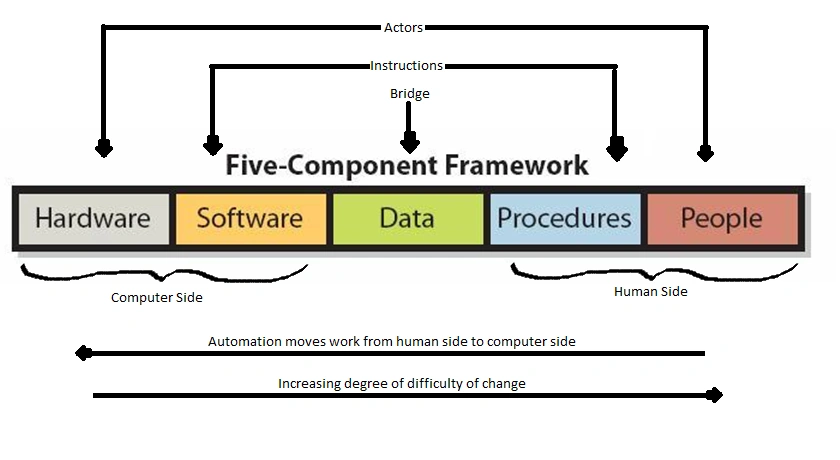
\includegraphics[width=0.9\textwidth]{5_thanh_phan_MIS.png}
    \caption{Sơ đồ mô hình 5 thành phần của hệ thống thông tin (MIS)}
    \label{fig:mis_5_components}
\end{figure}

\subsection{Vai trò của MIS trong quản lý doanh nghiệp}
Trong bối cảnh kỷ nguyên số (Digital Era), khi mà thông tin đã trở thành tài sản vô hình mang tính quyết định đến năng lực cạnh tranh, Hệ thống thông tin quản lý (MIS) đóng vai trò như một "hệ thần kinh trung ương" điều phối mọi hoạt động của doanh nghiệp. Vai trò của MIS được thể hiện rõ nét qua bốn khía cạnh chiến lược sau:

\textbf{Thứ nhất, phá vỡ các rào cản thông tin (Information Silos) và tích hợp liên chức năng.} 
Trong các mô hình quản trị truyền thống, dữ liệu thường bị cô lập tại từng phòng ban riêng biệt (nhân sự có dữ liệu của nhân sự, dự án có dữ liệu của dự án). MIS đóng vai trò như một cầu nối, tích hợp toàn bộ luồng dữ liệu phân tán này vào một cơ sở dữ liệu tập trung (Centralized Database). Điều này đảm bảo tính nhất quán của dữ liệu (Single Source of Truth), cho phép luồng thông tin được lưu thông xuyên suốt theo thời gian thực (Real-time), giúp các bộ phận dễ dàng phối hợp và tránh tình trạng xung đột thông tin.

\textbf{Thứ hai, hỗ trợ ra quyết định dựa trên dữ liệu (Data-Driven Decision Making).} 
Các cấp quản lý thường xuyên phải đối mặt với hàng loạt quyết định phức tạp, từ việc phân bổ nguồn lực, điều chỉnh tiến độ dự án, đến việc đánh giá năng lực nhân sự. Thay vì đưa ra quyết định dựa trên kinh nghiệm hoặc trực giác cá nhân (Gut-feeling), MIS cung cấp cho các nhà quản lý hệ thống Bảng điều khiển (Dashboards) trực quan. Những dữ liệu thô (ví dụ: số giờ làm việc, trạng thái hoàn thành task) sẽ được MIS tự động xử lý và chuyển hóa thành các chỉ số đánh giá thực hiện công việc (KPI). Từ đó, nhà quản lý có căn cứ khoa học, minh bạch và chính xác tuyệt đối để ra quyết định tưởng thưởng, xử phạt hoặc tái cấu trúc đội ngũ.

\textbf{Thứ ba, tối ưu hóa quy trình và nâng cao hiệu suất hoạt động (Operational Efficiency).} 
Việc ứng dụng MIS giúp doanh nghiệp tự động hóa (Automation) hàng loạt các tác vụ lặp đi lặp lại có tính quy luật. Những công việc tiêu tốn nhiều thời gian và dễ xảy ra sai sót do yếu tố con người như: nhắc nhở hạn chót công việc (Deadline), tổng hợp báo cáo thời gian làm việc (Timesheet), hay tính toán điểm số hiệu suất cuối tháng, nay đều được thực hiện ngầm bởi các tiến trình của hệ thống. Nhờ đó, nhân sự được giải phóng khỏi các công việc hành chính tẻ nhạt để tập trung vào các nghiệp vụ chuyên môn mang lại giá trị gia tăng cao hơn.

\textbf{Thứ tư, nhận diện rủi ro và quản trị sự thay đổi (Risk Management \& Change Control).} 
Một trong những giá trị cốt lõi nhất của MIS đối với người làm quản lý dự án là khả năng cảnh báo sớm. Thông qua việc liên tục đối chiếu giữa tiến độ kế hoạch (Planned) và tiến độ thực tế (Actual), hệ thống có khả năng tự động nhận diện các điểm nghẽn (Bottlenecks) hoặc các nguy cơ trễ hạn (Overdue/Risk Alert). Điều này chuyển đổi tư duy quản trị của doanh nghiệp từ thế "bị động khắc phục hậu quả" sang "chủ động phòng ngừa và điều hướng rủi ro", đảm bảo các dự án công nghệ luôn được hạ cánh an toàn theo đúng quỹ đạo ngân sách và thời gian đã cam kết.

\section{Quản lý dự án (Project Management) và phương pháp đánh giá}
\subsection{Cấu trúc phân rã công việc (WBS) và Sơ đồ Gantt}

Trong quản lý dự án hiện đại, đặc biệt là các dự án phát triển Hệ thống thông tin quản lý (MIS) có quy mô và độ phức tạp cao, việc kiểm soát phạm vi và thời gian là những yếu tố quyết định đến sự thành bại. Để hiện thực hóa điều này, hai công cụ kinh điển mang tính bổ trợ chặt chẽ cho nhau được áp dụng phổ biến là Cấu trúc phân rã công việc (Work Breakdown Structure - WBS) và Sơ đồ Gantt (Gantt Chart).

\textbf{1. Cấu trúc phân rã công việc (WBS) và tầm quan trọng tiền hệ thống}

Cấu trúc phân rã công việc (WBS) được định nghĩa là một công cụ phân chia có cấu trúc thứ bậc (hướng kết quả đầu ra) toàn bộ phạm vi công việc của một dự án thành các phần hành, gói công việc (Work Packages), nhiệm vụ (Tasks) và nhiệm vụ con (Sub-tasks) nhỏ hơn, có mức độ chi tiết tăng dần. Mục tiêu cốt lõi của WBS là bẻ gãy một mục tiêu lớn, trừu tượng thành các khối công việc cụ thể, có khả năng định lượng và quản lý độc lập.

Trước khi bắt tay vào xây dựng phần mềm hoặc triển khai một hệ thống MIS, việc thiết lập một sơ đồ WBS hoàn chỉnh là điều kiện tiên quyết mang tính sống còn vì các lý do sau:
\begin{itemize}
    \item \textbf{Ngăn ngừa rủi ro tràn phạm vi (Scope Creep):} Trong các dự án công nghệ, yêu cầu của khách hàng hoặc người dùng thường có xu hướng thay đổi và phình to liên tục. WBS đóng vai trò là một ranh giới pháp lý và kỹ thuật, định nghĩa rõ ràng những gì nằm trong và nằm ngoài phạm vi dự án, giúp đội ngũ phát triển tập trung vào các tính năng cốt lõi.
    \item \textbf{Cơ sở để ước lượng nguồn lực chính xác:} Một dự án lớn không thể ước lượng thời gian (Estimated Time) và chi phí một cách cảm tính. Khi công việc được chia nhỏ đến tầng thấp nhất (gói công việc), nhà quản lý có thể dễ dàng tính toán chính xác số giờ công cần thiết, ngân sách tương ứng và gán trách nhiệm cụ thể cho từng nhân sự phụ trách (Assignee).
    \item \textbf{Định hình kiến trúc và luồng dữ liệu phần mềm:} WBS cung cấp một cái nhìn tổng thể về các khối chức năng. Dựa vào cấu trúc cây của WBS, các kỹ sư hệ thống có thể thiết kế kiến trúc mô-đun phần mềm, các Endpoint API và cấu trúc các bảng trong cơ sở dữ liệu một cách logic và đồng bộ.
\end{itemize}

\textit{Ví dụ cụ thể về phân rã cấu trúc WBS cho một dự án xây dựng Website Quản trị Doanh nghiệp:}
Để minh họa cho lý thuyết trên, toàn bộ phạm vi dự án Website có thể được phân rã theo các cấp độ (Levels) như sau:
\begin{itemize}
    \item \textbf{Level 1 (Cấp dự án tổng):} Dự án xây dựng Website Quản trị Doanh nghiệp.
    \item \textbf{Level 2 (Cấp giai đoạn/Phân hệ lớn):}
        \begin{itemize}
            \item 1.0 Khảo sát \& Phân tích yêu cầu nghiệp vụ.
            \item 2.0 Thiết kế giao diện người dùng (UI/UX Design).
            \item 3.0 Phát triển mã nguồn (Coding/Development).
            \item 4.0 Kiểm thử hệ thống (System Testing).
            \item 5.0 Triển khai và bàn giao.
        \end{itemize}
    \item \textbf{Level 3 (Chi tiết hóa cấu phần - Xét nhánh 3.0 Phát triển mã nguồn):}
        \begin{itemize}
            \item 3.1 Thiết kế và cài đặt Cơ sở dữ liệu (Database Setup).
            \item 3.2 Phát triển các thành phần Front-end (Giao diện ReactJS).
            \item 3.3 Phát triển các thành phần Back-end API (Logic nền tảng .NET Core).
        \end{itemize}
    \item \textbf{Level 4 (Cấp gói công việc thấp nhất - Xét nhánh 3.3 Phát triển Back-end API):}
        \begin{itemize}
            \item 3.3.1 Xây dựng API xác thực và phân quyền người dùng (Auth API/JWT).
            \item 3.3.2 Xây dựng các Endpoint CRUD quản lý công việc (Task Management API).
            \item 3.3.3 Lập trình động cơ tính toán và tổng hợp điểm hiệu suất tự động (KPI Engine).
        \end{itemize}
 \end{itemize}

\textbf{2. Sơ đồ Gantt và nghệ thuật quản lý thời gian trực quan}

Sau khi cấu trúc WBS đã bóc tách tường tận các đầu việc, dữ liệu này sẽ được đổ vào Sơ đồ Gantt để thiết lập dòng thời gian. Sơ đồ Gantt là một dạng biểu đồ thanh ngang biểu diễn tiến độ thực hiện dự án theo thời gian. Trục tung chứa danh sách các nhiệm vụ (kế thừa trực tiếp từ sơ đồ cây WBS) và trục hoành hiển thị các mốc thời gian (ngày, tuần, tháng).

Sơ đồ Gantt hỗ trợ tối đa nhà quản lý trong việc kiểm soát và tối ưu hóa thời gian dự án thông qua các cơ chế:
\begin{itemize}
    \item \textbf{Trực quan hóa vòng đời và các cột mốc (Milestones):} Mỗi nhiệm vụ được biểu diễn bằng một thanh ngang, độ dài của thanh tương ứng với khoảng thời gian thực hiện (từ Start Date đến Due Date). Nhìn vào sơ đồ, toàn bộ đội ngũ có thể nắm bắt ngay lập tức công việc nào đang chạy song song, công việc nào làm cuốn chiếu, và khi nào đến hạn chốt các mốc quan trọng.
    \item \textbf{Quản lý chặt chẽ tính phụ thuộc của công việc (Task Dependencies):} Đây là giá trị cốt lõi nhất của sơ đồ Gantt. Trong phát triển phần mềm, các tác vụ thường có liên kết ràng buộc lẫn nhau, phổ biến nhất là quan hệ Finish-to-Start (FS) - ví dụ: Không thể tiến hành kiểm thử (Task B) nếu quá trình code Back-end (Task A) chưa hoàn thành. Sơ đồ Gantt biểu diễn các ràng buộc này bằng các đường mũi tên kết nối giữa các thanh ngang.
    \item \textbf{Xác định Đường găng (Critical Path) và tự động hóa đồng bộ trễ hạn:} Thông qua các mối quan hệ phụ thuộc, hệ thống quản lý tích hợp sơ đồ Gantt có thể tự động tính toán ra Đường găng – chuỗi các nhiệm vụ có tổng thời gian dài nhất và không có thời gian dự phòng. Nếu bất kỳ một nhiệm vụ nào trên Đường găng này bị chậm trễ, toàn bộ ngày hoàn thành của dự án sẽ bị đẩy lùi. Khi một Task tiền quyết bị chuyển trạng thái trễ hạn (Overdue) trên bảng Kanban, thuật toán hệ thống sẽ tự động kích hoạt tính toán lại, đẩy lùi thời gian dự kiến của các Task kế tiếp trên sơ đồ Gantt theo thời gian thực mà không cần con người can thiệp thủ công.
\end{itemize}

\subsubsection{Cấu trúc phân rã công việc (WBS) và Sơ đồ Gantt}
Cấu trúc phân rã công việc (WBS - Work Breakdown Structure) và sơ đồ Gantt là hai công cụ cốt lõi trong quản lý tiến độ dự án...

\begin{figure}[H]
    \centering
    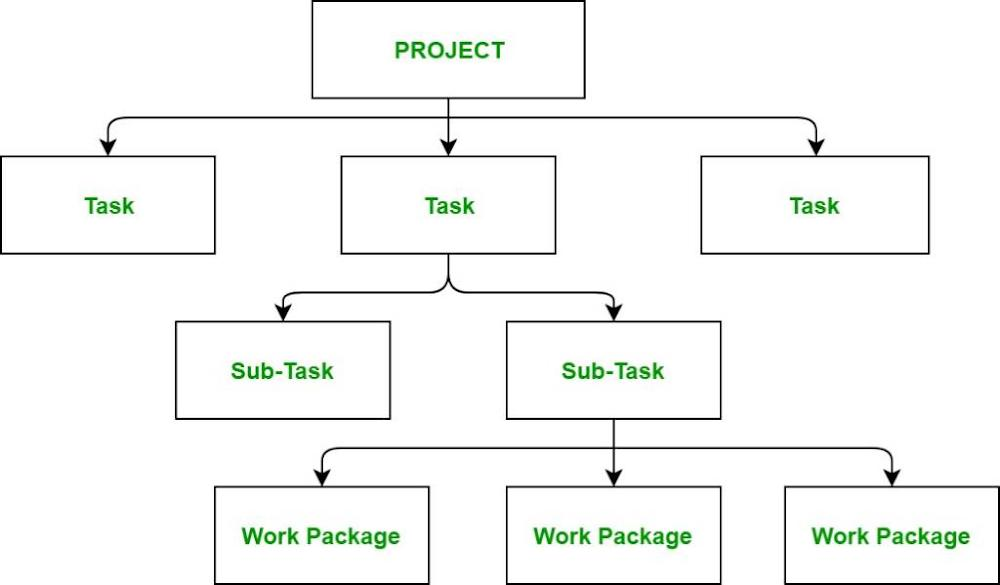
\includegraphics[width=0.75\textwidth]{WBS.png} 
    \caption{Ví dụ về cấu trúc phân tầng tổng quát của sơ đồ WBS (Nguồn: GeeksforGeeks)}
    \label{fig:wbs_generic}
\end{figure}

\begin{figure}[H]
    \centering
    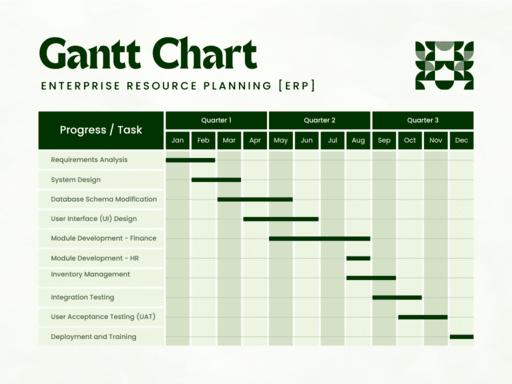
\includegraphics[width=0.8\textwidth]{gantt_theory_diagram.png} 
    \caption{Ví dụ về sơ đồ Gantt trong quản lý tiến độ dự án hệ thống ERP (Nguồn: GeeksforGeeks)}
    \label{fig:gantt_erp}
\end{figure}


\subsection{Bảng Kanban trong theo dõi tiến độ Agile}

Bắt nguồn từ hệ thống sản xuất tinh gọn (Lean Manufacturing) của Toyota vào cuối thập niên 1940, Kanban đã vượt ra khỏi ranh giới của ngành công nghiệp ô tô để trở thành một trong những phương pháp luận quản lý dự án linh hoạt (Agile) phổ biến nhất trong lĩnh vực kỹ thuật phần mềm. Nếu cấu trúc WBS và sơ đồ Gantt thiên về hoạch định và kiểm soát vĩ mô, thì bảng Kanban lại đóng vai trò là công cụ quản lý vi mô xuất sắc, tập trung vào việc tối ưu hóa dòng chảy công việc (Workflow) hàng ngày của toàn bộ đội ngũ.

Triết lý vận hành của phương pháp Kanban được xây dựng dựa trên hai nguyên tắc nền tảng:

\textbf{Thứ nhất, trực quan hóa luồng công việc (Visualizing Workflow).} Bảng Kanban đóng vai trò như một bộ tản nhiệt thông tin (Information Radiator) cho toàn bộ dự án. Mọi gói công việc (Task) sau khi được phân rã từ WBS sẽ được ánh xạ thành một thẻ dữ liệu (Card) trên bảng. Bảng Kanban tiêu chuẩn được chia thành các cột đại diện cho các trạng thái của một chu kỳ xử lý, cơ bản nhất bao gồm: Cần làm (To Do), Đang thực hiện (Doing), và Đã hoàn thành (Done). Đối với các hệ thống MIS có tính chất kiểm soát khắt khe, các trạng thái này có thể được tùy biến mở rộng thêm như Chờ phê duyệt (Pending Review) hay Trễ hạn (Overdue). Bằng cách trực quan hóa mọi tác vụ, cấp quản lý và từng nhân sự có thể nhìn thấu suốt toàn bộ tiến trình dự án theo thời gian thực (Real-time). Việc nhận biết ai đang làm gì, tiến độ ra sao được thể hiện rõ ràng thông qua việc dịch chuyển các thẻ từ trái sang phải xuyên suốt quy trình như minh họa tại Hình \ref{fig:kanban_misa}.

\begin{figure}[H]
    \centering
    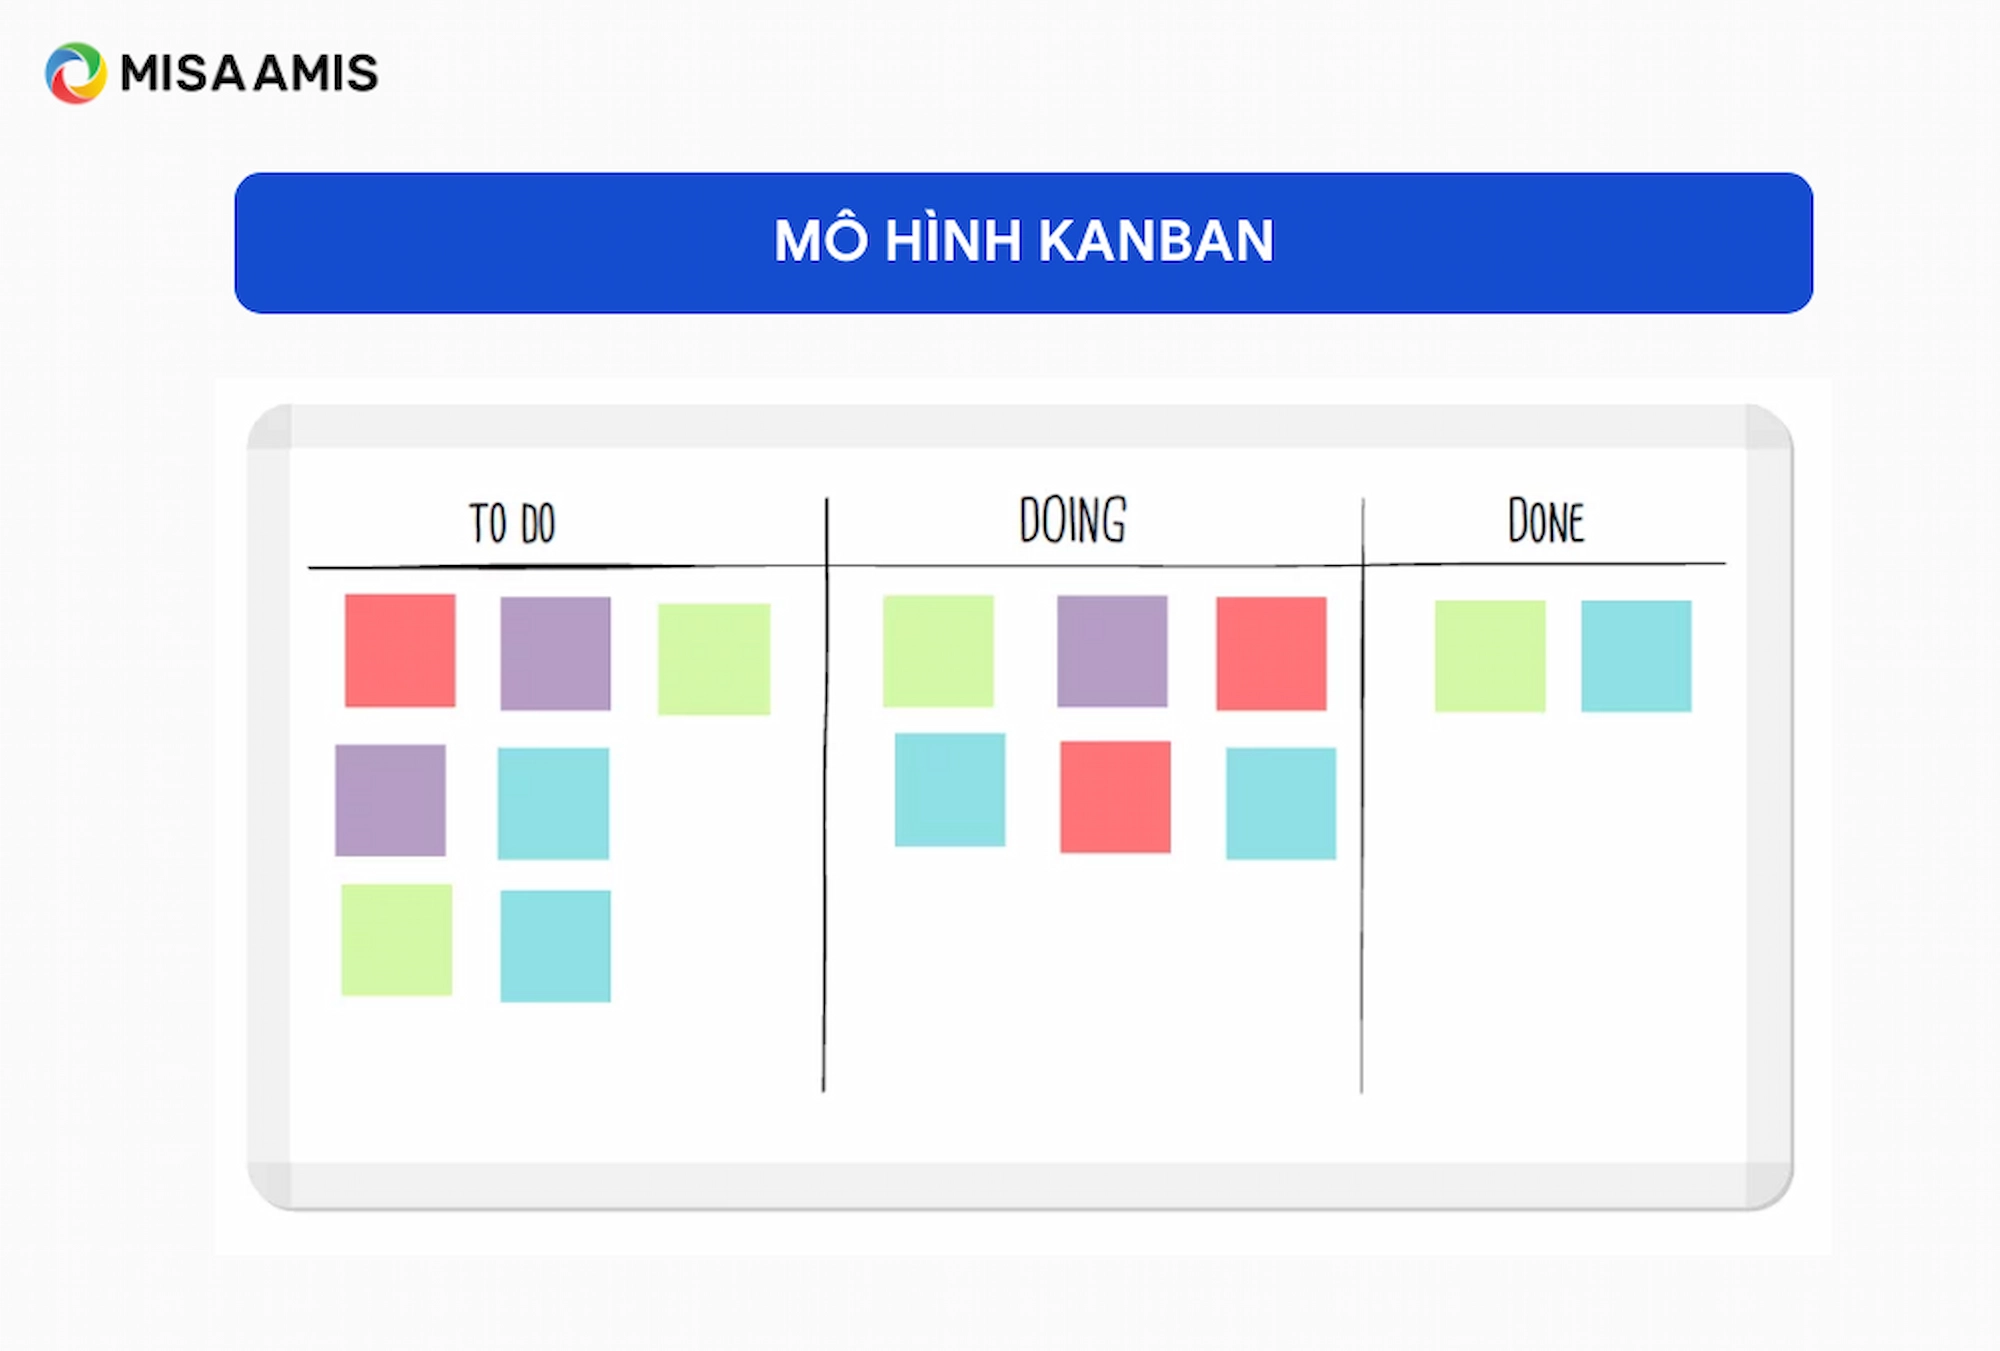
\includegraphics[width=0.85\textwidth]{Kaban_flow.png} 
    \caption{Minh họa giao diện bảng quản lý công việc theo mô hình Kanban (Nguồn: MISA AMIS)}
    \label{fig:kanban_misa}
\end{figure}

\textbf{Thứ hai, giới hạn công việc đang tiến hành (Limit Work-in-Progress - WIP Limit).} Đây là nguyên lý cốt lõi tạo nên sức mạnh tối ưu hóa của Kanban. WIP Limit là việc thiết lập số lượng thẻ tối đa được phép tồn tại trong một cột trạng thái nhất định (thường là cột "Doing") tại cùng một thời điểm. Trong môi trường công nghệ, việc một lập trình viên phải chuyển đổi bối cảnh liên tục (Context Switching) giữa quá nhiều Task sẽ làm suy giảm nghiêm trọng năng suất, gây phân tán tư tưởng và gia tăng tỷ lệ phát sinh lỗi (Bugs). Bằng cách áp đặt WIP Limit, Kanban ép buộc đội ngũ phải hoàn thành dứt điểm công việc hiện tại trước khi áp dụng cơ chế "Kéo" (Pull System) để nhận một công việc mới vào luồng. Điều này không chỉ giúp duy trì sự tập trung cao độ mà còn giúp người quản lý dễ dàng phát hiện các "nút thắt cổ chai" (Bottlenecks) – nơi công việc bị dồn ứ do thiếu hụt nguồn lực hoặc vướng mắc kỹ thuật, từ đó có phương án can thiệp và san sẻ tải lượng kịp thời.

\textbf{Sự phù hợp của Kanban đối với các đội nhóm phát triển phần mềm hiện nay:}

Trong bối cảnh kỷ nguyên công nghệ thay đổi liên tục, các yêu cầu của khách hàng thường xuyên biến động (Volatile Requirements), phương pháp Kanban thể hiện sự linh hoạt vượt trội so với các mô hình quy trình tuyến tính thác nước (Waterfall) truyền thống. Khác với mô hình Scrum yêu cầu phải đóng băng phạm vi công việc trong một vòng lặp cố định (Sprint), Kanban vận hành theo cơ chế phân phối liên tục (Continuous Delivery). Khi có yêu cầu thay đổi tính năng hay phát sinh lỗi đột xuất, Quản lý dự án (Manager) chỉ cần bổ sung các thẻ mới vào cột "To Do" và điều chỉnh mức độ ưu tiên (Priority). Đội ngũ phát triển sẽ tuần tự xử lý các tác vụ này một cách mượt mà mà không làm phá vỡ cấu trúc nhịp độ chung của hệ thống.

Bên cạnh đó, Kanban đề cao tính minh bạch và tinh thần làm việc cộng tác (Collaboration). Khi được số hóa và tích hợp vào một Hệ thống thông tin quản lý (MIS), bảng Kanban sẽ tự động ghi vết (Audit Log) các lịch sử thao tác kéo thả, thời gian bắt đầu và kết thúc của từng thẻ (Cycle Time \& Lead Time). Đây chính là nguồn dữ liệu định lượng gốc vô cùng quan trọng để hệ thống tiến hành các thuật toán đo lường hiệu suất thực tế (Actual Log-time), làm cơ sở cho việc tính toán điểm KPI cuối tháng một cách khách quan và công bằng nhất.



\subsection{Đánh giá hiệu suất nhân sự bằng chỉ số KPI}

\textbf{1. Khái niệm KPI và tầm quan trọng của dữ liệu thực tế}

Chỉ số đánh giá thực hiện công việc (Key Performance Indicator - KPI) là một công cụ đo lường giá trị định lượng, được sử dụng để đánh giá mức độ hiệu quả của một tổ chức, bộ phận hoặc cá nhân trong việc đạt được các mục tiêu chiến lược đã đề ra. Trong lĩnh vực Kỹ thuật phần mềm và Quản lý dự án công nghệ, KPI không chỉ là một con số dùng để tính lương cuối tháng, mà là một cơ sở dữ liệu phản chiếu sức khỏe của toàn bộ đội ngũ phát triển.

Bản chất của hệ thống KPI hiện đại đòi hỏi sự minh bạch tuyệt đối và phải được xây dựng dựa trên dữ liệu thực tế (Data-driven). Trong các phương pháp quản lý lỗi thời, việc đánh giá nhân sự thường bị chi phối bởi "hiệu ứng hào quang" (Halo Effect) – nơi nhà quản lý đánh giá hiệu suất dựa trên cảm tính, trí nhớ hoặc sự thiên vị cá nhân. Điều này dễ dẫn đến môi trường làm việc độc hại, gây bất mãn và làm chảy máu chất xám. Khi tích hợp KPI vào một Hệ thống thông tin quản lý (MIS), mọi chỉ số đều được trích xuất trực tiếp từ các dữ liệu thô (Raw Data) sinh ra trong quá trình làm việc hàng ngày: từ số giờ thao tác trên hệ thống (Log-time), thời điểm chuyển trạng thái thẻ trên bảng Kanban, cho đến tỷ lệ trễ hạn trên sơ đồ Gantt. Sự minh bạch này thiết lập một "nguồn sự thật duy nhất" (Single Source of Truth), giúp nhân viên thấu hiểu rõ ràng lý do đằng sau điểm số của mình và tự chủ động điều chỉnh năng suất làm việc.

\textbf{2. Bộ tiêu chí đánh giá KPI dành cho nhân sự kỹ thuật}

Việc đo lường năng suất của một Lập trình viên (Developer) hay Chuyên viên kiểm thử (Tester) phức tạp hơn rất nhiều so với các công việc hành chính thông thường. Không thể đo lường giá trị của một lập trình viên thông qua số dòng code họ viết ra, bởi một thuật toán tối ưu thường ngắn gọn và tốn ít dòng code hơn một thuật toán kém hiệu quả. Do đó, hệ thống KPI cần được tổng hợp đa chiều dựa trên các trọng số về Tiến độ, Hiệu suất, Khối lượng và Chất lượng.



\begin{table}[H]
    \centering
    \renewcommand{\arraystretch}{1.5}
    \begin{tabularx}{\textwidth}{|C{3.5cm}|C{5cm}|X|}
    \hline
    \textbf{Tên chỉ số} & \textbf{Công thức tính} & \multicolumn{1}{c|}{\textbf{Ý nghĩa}} \\
    \hline
    \textbf{Tiến độ (Timeliness)} & $\frac{\text{Số Task hoàn thành đúng hạn}}{\text{Tổng số Task được giao}} \times 100\%$ & Đo lường mức độ cam kết về mặt thời gian, khả năng quản trị rủi ro cá nhân và tuân thủ \textit{Deadline} của dự án. \\
    \hline
    \textbf{Hiệu suất (Efficiency)} & $\frac{\text{Tổng thời gian dự kiến (Est)}}{\text{Tổng thời gian thực tế (Log-time)}} \times 100\%$ & Phản ánh tốc độ và kỹ năng giải quyết vấn đề. Tỷ lệ $>100\%$ cho thấy nhân sự hoàn thành công việc nhanh hơn thời gian hệ thống dự kiến. \\
    \hline
    \textbf{Khối lượng (Capacity)} & $\frac{\text{Tổng giờ thực tế (Log-time)}}{\text{Số giờ làm chuẩn trong tháng}} \times 100\%$ & Đánh giá cường độ làm việc và mức độ cống hiến. Nếu tỷ lệ này vượt quá $110\%$, nhân sự đang rơi vào trạng thái quá tải (\textit{Overload}) cần được san sẻ công việc. \\
    \hline
    \textbf{Chất lượng (Quality)} & Điểm đánh giá trực tiếp từ Quản lý (Thang điểm 100) & Đánh giá các yếu tố khó định lượng hoàn toàn bằng máy như: thái độ phối hợp (\textit{Teamwork}), số lượng lỗi (\textit{Bugs}) phát sinh sau khi Test, và khả năng hỗ trợ đồng nghiệp. \\
    \hline
    \end{tabularx}
    \caption{Tóm tắt các tiêu chí đánh giá KPI cho nhân sự kỹ thuật}
    \label{tab:kpi_criteria}
\end{table}

\textbf{3. Các sai lầm thường gặp khi áp dụng KPI trong dự án phần mềm}

Dù là một công cụ mạnh mẽ, việc triển khai KPI sai cách có thể biến hệ thống thành một cỗ máy tạo áp lực. Trong thực tiễn quản lý, các tổ chức thường mắc phải hai sai lầm chí mạng sau:

\begin{itemize}
    \item \textbf{Đo lường cảm tính và sử dụng "Chỉ số ảo" (Vanity Metrics):} Nhà quản lý thường nhầm lẫn giữa nỗ lực (Effort) và kết quả (Outcome). Việc đánh giá KPI dựa trên số giờ ngồi tại văn phòng thay vì giá trị phần mềm được bàn giao sẽ khuyến khích văn hóa "làm việc đối phó". Đồng thời, nếu không có một hệ thống MIS thu thập dữ liệu Log-time độc lập, việc đánh giá cuối tháng sẽ chỉ dựa vào trí nhớ của Manager, gây ra sự sai lệch nghiêm trọng.
    \item \textbf{Thiết lập mục tiêu phi thực tế (Unrealistic Goals) và thiếu cơ chế ngoại lệ:} Quản lý dự án thường kỳ vọng nhân sự sẽ đạt $100\%$ công suất làm việc liên tục. Tuy nhiên, trong phát triển phần mềm, nhân sự cần thời gian cho việc chuyển đổi bối cảnh (Context Switching), sửa các lỗi nợ kỹ thuật (Technical Debt) hoặc họp hành. Nếu hệ thống KPI áp đặt các chỉ tiêu quá khắc nghiệt mà không có cơ chế "Hệ số vượt khó" (Thưởng Overload) khi nhân sự phải gánh vác khối lượng công việc khổng lồ, hệ thống sẽ trực tiếp dẫn đến tình trạng kiệt sức (Burnout) và phá vỡ cấu trúc của toàn bộ đội ngũ.
\end{itemize} 

% --- CHƯƠNG 2 ---
\chapter{PHÂN TÍCH VÀ THIẾT KẾ HỆ THỐNG}

\section{Khảo sát hiện trạng và Xác định bài toán}
\subsection{Giới thiệu tổ chức và bối cảnh áp dụng}

Đối tượng khảo sát và ứng dụng của đề tài là một doanh nghiệp công nghệ thông tin quy mô tầm trung (SME), hoạt động chủ yếu trong lĩnh vực gia công phần mềm (IT Outsourcing) và phát triển sản phẩm công nghệ (Product Development). Với quy mô nhân sự dao động từ 50 đến 100 người, cơ cấu tổ chức của doanh nghiệp được phân tách thành các bộ phận chuyên môn hóa cao nhằm đảm bảo luồng công việc diễn ra xuyên suốt . Cấu trúc cốt lõi bao gồm: Ban Giám đốc (C-Level), Khối Quản trị Dự án (Project Management Office - PMO), Khối Kỹ thuật (bao gồm các đội nhóm Developer, Tester/QA, Business Analyst) và Khối Hành chính - Nhân sự (HR/Admin) . Đội ngũ nhân sự làm việc theo mô hình linh hoạt (Hybrid) và áp dụng chặt chẽ phương pháp luận phát triển phần mềm Agile . Mô hình phân cấp và các kênh tương tác báo cáo giữa các khối chức năng này được trực quan hóa cụ thể thông qua Sơ đồ cơ cấu tổ chức tại Hình \ref{fig:org_chart}.

\begin{figure}[H]
    \centering
    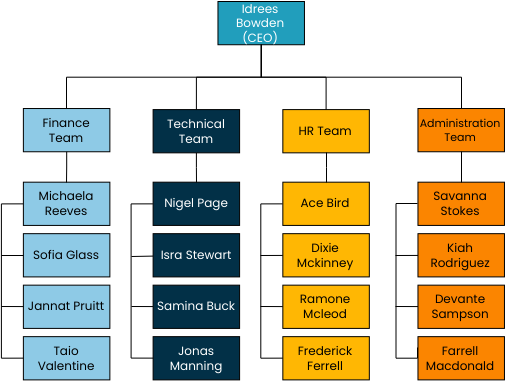
\includegraphics[width=0.8\textwidth]{org_chart.png} % Hãy lưu ảnh này với tên company-org-chart.png rồi upload lên LaTeX
    \caption{Sơ đồ phân cấp cơ cấu tổ chức doanh nghiệp SME điển hình (Nguồn: online.visual-paradigm.com)}
    \label{fig:org_chart}
\end{figure}

Trong giai đoạn đầu thành lập, việc vận hành tổ chức dựa trên các công cụ quản lý rời rạc như bảng tính Excel (để lập kế hoạch và WBS), các ứng dụng OTT như Zalo/Telegram (để giao việc, báo cáo hàng ngày) hay Google Forms (để chấm công) vẫn tạm thời đáp ứng được nhu cầu. Tuy nhiên, khi doanh nghiệp bước vào giai đoạn tăng trưởng nóng và mở rộng quy mô (Scaling-up), số lượng dự án tăng vọt kéo theo sự bùng nổ về khối lượng dữ liệu nghiệp vụ. Mô hình quản lý thủ công nhanh chóng chạm ngưỡng giới hạn và bộc lộ những điểm nghẽn (Bottlenecks) mang tính hệ thống.

Điểm nghẽn nghiêm trọng nhất là tình trạng "phân mảnh dữ liệu" (Data Fragmentation). Cấp quản lý rơi vào trạng thái "mù thông tin" (Information Blindness) cục bộ khi không thể bao quát toàn cảnh tiến độ dự án theo thời gian thực (Real-time). Việc theo dõi trạng thái của từng gói công việc (Task) trở nên hỗn loạn, dẫn đến nguy cơ trễ hạn (Overdue) dây chuyền không được cảnh báo sớm. Đồng thời, quá trình khai báo thời gian làm việc thực tế (Log-time) phụ thuộc hoàn toàn vào tính tự giác và trí nhớ của nhân viên kỹ thuật, gây ra sai số lớn và thất thoát giờ công của tổ chức.

Hệ lụy lớn nhất của mô hình cũ đổ dồn vào khâu đánh giá hiệu suất nhân sự (KPI) cuối tháng. Do thiếu vắng một "nguồn sự thật duy nhất" (Single Source of Truth) lưu trữ dữ liệu hiệu suất khách quan, việc chấm điểm KPI biến thành một gánh nặng hành chính khổng lồ. Quá trình này bị chi phối nặng nề bởi cảm tính và trí nhớ của người quản lý (Halo Effect). Sự thiếu minh bạch trong định lượng kết quả không chỉ gây ra tâm lý bất mãn, làm giảm động lực cống hiến của đội ngũ kỹ sư, mà còn tước đi của Ban Giám đốc những cơ sở dữ liệu xác đáng để ra quyết định chiến lược về thăng tiến, lương thưởng hay tái cấu trúc nguồn lực.

Đứng trước bờ vực của sự khủng hoảng quản trị, việc chuyển đổi số toàn diện luồng quy trình nội bộ không còn là một lựa chọn tối ưu hóa mà đã trở thành mệnh lệnh mang tính sống còn. Doanh nghiệp đặt ra yêu cầu cấp thiết về việc xây dựng và ứng dụng một Hệ thống thông tin quản lý (MIS) chuyên biệt. Hệ thống này phải đóng vai trò như một "hệ thần kinh trung ương", kết nối thông suốt toàn bộ quy trình: từ khâu khởi tạo dự án, phân rã WBS, điều phối công việc trực quan trên bảng Kanban, cho đến việc tự động hóa quá trình phê duyệt Log-time và tổng hợp điểm KPI một cách minh bạch, chính xác tuyệt đối.

\subsection{Thành phần hệ thống thông tin (Cứng, Mềm, Con người, Quy trình, Dữ liệu)}

Để đánh giá toàn diện mức độ trì trệ của mô hình quản lý hiện tại và làm nổi bật sự cấp thiết phải chuyển đổi số, chúng ta cần tiến hành "giải phẫu" tổ chức thông qua lăng kính của 5 thành phần cấu thành nên một hệ thống thông tin. Sự thiếu đồng bộ và lạc hậu trong bất kỳ thành phần nào cũng sẽ trở thành điểm nghẽn (Bottleneck) kéo lùi hiệu suất của toàn bộ cỗ máy.



\begin{table}[H]
    \centering
    \renewcommand{\arraystretch}{1.5}
    \begin{tabularx}{\textwidth}{|C{2.5cm}|X|X|}
    \hline
    \textbf{Thành phần} & \multicolumn{1}{c|}{\textbf{Hiện trạng (Quản lý thủ công)}} & \multicolumn{1}{c|}{\textbf{Hạn chế \& Rủi ro}} \\
    \hline
    \textbf{Phần cứng (Hardware)} & Dữ liệu dự án được lưu trữ phân tán cục bộ (Local Storage) trên các máy tính cá nhân của từng Quản lý dự án (Manager). & Rủi ro mất mát dữ liệu nội bộ rất cao khi xảy ra sự cố hỏng hóc thiết bị. Khó khăn trong việc chia sẻ và đồng bộ hóa tài nguyên. \\
    \hline
    \textbf{Phần mềm (Software)} & Sử dụng chắp vá một hệ sinh thái các ứng dụng rời rạc: Excel để lập WBS, Zalo/Telegram để giao việc và báo cáo tiến độ, Google Sheets để chấm công. & Gây ra "Hội chứng phân mảnh dữ liệu" (Data Fragmentation). Không có khả năng liên kết thông tin tự động, làm suy giảm nghiêm trọng trải nghiệm người dùng (UX) khi phải chuyển đổi liên tục giữa các App. \\
    \hline
    \textbf{Dữ liệu (Data)} & Dữ liệu đầu vào (\textit{Input}) bị trùng lặp, thiếu tính đồng nhất và định dạng không chuẩn hóa. Dữ liệu giờ làm (\textit{Log-time}) mang tính chủ quan. & Vi phạm nguyên tắc "Nguồn sự thật duy nhất" (\textit{Single Source of Truth}). Dữ liệu rác (\textit{Garbage In}) khiến việc tự động hóa tính toán KPI là điều bất khả thi (\textit{Garbage Out}). \\
    \hline
    \textbf{Quy trình (Process)} & Vận hành hoàn toàn bằng sức người. Quản lý phải tự ghi nhớ để nhắc nhở \textit{Deadline}, tự cộng trừ file Excel để tính lương và KPI cuối tháng. & Quy trình bị phụ thuộc vào trí nhớ cá nhân, dẫn đến tình trạng "ngâm" hồ sơ, quên duyệt giờ làm, gây ách tắc luồng công việc và sai sót trong tính toán. \\
    \hline
    \textbf{Con người (People)} & Quản lý bị quá tải bởi các công việc hành chính tẻ nhạt. Nhân sự kỹ thuật bất mãn vì cơ chế đánh giá thiếu minh bạch, phụ thuộc vào cảm tính. & Năng suất lao động tổng thể sụt giảm. Môi trường làm việc thiếu công bằng làm gia tăng tỷ lệ nghỉ việc (\textit{Turnover Rate}), chảy máu chất xám. \\
    \hline
    \end{tabularx}
    \caption{Khảo sát và đánh giá 5 thành phần hệ thống thông tin hiện tại}
    \label{tab:five_components_survey}
\end{table}

Sự đứt gãy giữa các thành phần nêu trên tạo ra một vòng lặp ác tính. Khi phần mềm không tích hợp, dữ liệu sẽ bị phân mảnh; khi dữ liệu phân mảnh, quy trình sẽ phải dựa vào sức người để chắp vá; và khi con người phải gánh vác quá nhiều thao tác thủ công, sai sót là hệ quả tất yếu. Điều này khẳng định tổ chức không thể giải quyết bài toán quản trị chỉ bằng cách mua thêm một phần mềm chat hay nâng cấp máy tính, mà bắt buộc phải tái cấu trúc toàn diện thông qua một nền tảng MIS tập trung.

\subsection{Mục tiêu và phạm vi của hệ thống MIS}

Dựa trên kết quả khảo sát thực trạng và sự thấu hiểu những nỗi đau (Pain points) của doanh nghiệp, dự án "Hệ thống thông tin quản lý tiến độ công việc và đánh giá KPI tự động" được định hình với lộ trình chiến lược rõ ràng, chia làm các mục tiêu ngắn hạn và dài hạn cụ thể:

\textbf{1. Mục tiêu ngắn hạn (Giải quyết điểm nghẽn vận hành)}
\begin{itemize}
    \item \textbf{Số hóa và trực quan hóa luồng công việc:} Thay thế hoàn toàn Excel bằng một nền tảng tập trung. Cho phép phân rã cấu trúc dự án (WBS) đa cấp độ và điều phối công việc hàng ngày thông qua giao diện Bảng kéo thả (Kanban Board) và Sơ đồ tiến độ (Gantt Chart).
    \item \textbf{Chuẩn hóa luồng chấm công (Log-time):} Xây dựng "Trung tâm phê duyệt một cửa", bắt buộc nhân sự phải đính kèm minh chứng (Link tài liệu, Commit code) khi khai báo số giờ làm việc thực tế, loại bỏ tình trạng báo cáo gian lận hoặc cảm tính.
    \item \textbf{Tự động hóa đánh giá KPI:} Lập trình và tích hợp "Động cơ tính toán" (KPI Engine) chạy độc lập vào cuối mỗi kỳ đánh giá. Thuật toán sẽ tự động trích xuất dữ liệu Log-time đã được duyệt để tính toán ra điểm số dựa trên 4 trụ cột: Tiến độ, Hiệu suất, Khối lượng và Chất lượng.
\end{itemize}

\textbf{2. Mục tiêu dài hạn (Nâng tầm quản trị chiến lược)}
\begin{itemize}
    \item \textbf{Xây dựng văn hóa Data-driven:} Chuyển đổi tư duy quản trị của tổ chức từ việc "đoán định dựa trên kinh nghiệm" sang "ra quyết định dựa trên dữ liệu". Các Bảng điều khiển (Dashboards) sẽ đóng vai trò cảnh báo sớm các dự án có rủi ro trễ hạn.
    \item \textbf{Hoàn thiện hệ sinh thái quản trị khép kín:} Xây dựng các cổng kết nối API mở (Open API) để trong tương lai có thể đồng bộ hóa dữ liệu điểm KPI trực tiếp sang các Hệ thống Quản trị Nguồn nhân lực (HRM) và Phần mềm Kế toán (ERP), tự động hóa quy trình tính lương (Payroll) mà không cần xuất nhập file thủ công.
\end{itemize}

\textbf{3. Phạm vi triển khai của hệ thống}
Để đảm bảo tính khả thi trong khuôn khổ một đồ án, phạm vi của hệ thống (System Boundary) được khoanh vùng tập trung vào các lõi nghiệp vụ quản lý dự án nội bộ. Cụ thể:
\begin{itemize}
    \item \textbf{Nghiệp vụ trong phạm vi (In-scope):} Quản trị vòng đời tài khoản và phân quyền người dùng (Role-based Access Control); Quản lý vòng đời dự án (WBS, Kanban, Gantt); Quản lý thời gian làm việc cá nhân (Timesheet/Log-time); và Xử lý thuật toán đánh giá KPI tự động.
    \item \textbf{Nghiệp vụ ngoài phạm vi (Out-of-scope):} Hệ thống không xử lý các luồng nghiệp vụ liên quan đến Thu/Chi tài chính dự án, không bao gồm chức năng Quản lý quan hệ khách hàng (CRM) và không xử lý nghiệp vụ Tuyển dụng nhân sự.
\end{itemize}

Sơ đồ ngữ cảnh (System Context Diagram - DFD cấp 0) đóng vai trò định vị ranh giới của toàn bộ hệ thống quản lý thông tin dự án và KPI, đồng thời làm rõ các luồng thông tin tương tác giữa hệ thống với các tác nhân thực tế bao gồm Nhân viên (Employee), Quản lý dự án (Project Manager) và Quản trị viên (Administrator). Toàn bộ kiến trúc luồng dữ liệu này được trực quan hóa chi tiết tại Hình \ref{fig:system_context_tikz}.

\begin{figure}[H]
    \centering
    \begin{tikzpicture}[
        box/.style={rectangle, draw=black, thick, fill=white, minimum width=2.8cm, minimum height=1.3cm, align=center},
        circle_node/.style={circle, draw=black, thick, fill=white, minimum size=3.5cm, align=center},
        arrow/.style={-{Stealth[scale=1.2]}, thick}
    ]
        % Khởi tạo các Node với tọa độ cố định để tránh chồng lấn
        \node[circle_node] (sys) at (0,0) {Project \& KPI\\Management\\System (MIS)};
        \node[box] (emp) at (-6.5,0) {Employee};
        \node[box] (pm) at (6.5,0) {Project\\Manager};
        \node[box] (admin) at (0,-3.8) {Administrator};

        % Luồng dữ liệu giữa Employee và System (Nới rộng khoảng cách)
        \draw[arrow] ([yshift=4mm]emp.east) -- node[above, font=\small] {Log-time / Kanban Status} ([yshift=4mm]sys.west);
        \draw[arrow] ([yshift=-4mm]sys.west) -- node[below, font=\small] {Personal KPI / Schedule} ([yshift=-4mm]emp.east);

        % Luồng dữ liệu giữa PM và System (Nới rộng khoảng cách)
        \draw[arrow] ([yshift=4mm]pm.west) -- node[above, font=\small] {WBS / Gantt Plans / KPI Weight} ([yshift=4mm]sys.east);
        \draw[arrow] ([yshift=-4mm]sys.east) -- node[below, font=\small] {Performance Reports} ([yshift=-4mm]pm.west);

        % Luồng dữ liệu giữa Admin và System (Đẩy hẳn xuống dưới)
        \draw[arrow] ([xshift=-4mm]admin.north) -- node[left, font=\small, align=center] {Account\\Configuration} ([xshift=-4mm]sys.south);
        \draw[arrow] ([xshift=4mm]sys.south) -- node[right, font=\small, align=center] {System Logs} ([xshift=4mm]admin.north);
    \end{tikzpicture}
    \caption{Sơ đồ ngữ cảnh phạm vi hệ thống quản lý dự án và KPI (DFD Cấp 0) (Nguồn: Tác giả tự xây dựng)}
    \label{fig:system_context_tikz}
\end{figure}

\section{Phân tích yêu cầu hệ thống}
\subsection{Các tác nhân (Actors) và Phân quyền người dùng (Roles)}

Trong kiến trúc bảo mật của Hệ thống thông tin quản lý (MIS), việc thiết lập cơ chế Phân quyền dựa trên vai trò (Role-Based Access Control - RBAC) là yếu tố cốt lõi nhằm đảm bảo tính toàn vẹn dữ liệu, an toàn thông tin và phân luồng nghiệp vụ chính xác. Cơ chế này tuân thủ nguyên tắc "đặc quyền tối thiểu" (Principle of Least Privilege), nghĩa là mỗi tài khoản chỉ được hệ thống cấp phát các đặc quyền truy cập và thao tác vừa đủ để hoàn thành chức năng công việc được giao. 

Dựa trên kết quả khảo sát quy trình vận hành của tổ chức, hệ thống được thiết kế xoay quanh 3 nhóm tác nhân (Actors) cốt lõi:

\textbf{1. Quản trị viên hệ thống (Admin):} 
Đóng vai trò là người thiết lập nền tảng kỹ thuật và giám sát an ninh (Security and System Configuration). Nhằm đảm bảo tính độc lập và khách quan, Admin tuyệt đối không can thiệp vào các luồng nghiệp vụ kinh doanh hàng ngày như tạo dự án hay chấm điểm KPI. Trách nhiệm của Admin tập trung vào việc quản trị vòng đời tài khoản (cấp mới, phân quyền, khóa tài khoản nhân sự nghỉ việc), định nghĩa cơ cấu phòng ban và cấu hình các bộ tham số vận hành chung (như số giờ làm việc chuẩn trong tháng, các định mức hệ số phạt trễ hạn). Đồng thời, Admin là người duy nhất có quyền trích xuất Nhật ký thao tác (Audit Logs) để truy vết mọi hành vi thêm, sửa, xóa dữ liệu nhạy cảm trên hệ thống.

\textbf{2. Quản lý dự án (Manager):} 
Là "nút thắt" trung tâm (Central Hub) điều phối toàn bộ vòng đời dự án và kiểm soát chất lượng nhân sự. Manager được cấp quyền quản trị (Administer) đối với các dự án do mình trực tiếp phụ trách. Trách nhiệm của họ trải dài từ khâu bóc tách cấu trúc phân rã công việc (WBS), thiết lập các cột mốc trên Sơ đồ Gantt, gán Task cho nhân viên (Assignee), cho đến việc xử lý các luồng phê duyệt (Duyệt/Từ chối giờ làm thực tế Log-time). Ở cuối chu kỳ, Manager là tác nhân trực tiếp đánh giá các tiêu chí ngoại lệ (Thưởng Overload, Chấp nhận báo cáo rủi ro) và xác nhận "Chốt sổ" bảng điểm KPI để chuyển sang bộ phận Kế toán.

\textbf{3. Nhân sự thực thi (Employee):} 
Là lực lượng sản xuất trực tiếp (Developer, Tester, BA) hoạt động ở tầng vi mô của hệ thống. Quyền truy cập của Employee được hệ thống giới hạn chặt chẽ theo cơ chế hiển thị dữ liệu (Data Visibility) – họ chỉ có thể nhìn thấy và tương tác với các Dự án/Gói công việc mà họ được đích danh gán vào. Quyền hạn của Employee bao gồm việc thao tác kéo thả trạng thái công việc trên Bảng Kanban, khai báo số giờ làm việc thực tế (Log-time) bắt buộc đính kèm minh chứng tài liệu/mã nguồn, gửi yêu cầu xin gia hạn tiến độ và theo dõi Bảng điều khiển hiệu suất (KPI Dashboard) của riêng cá nhân mình.

Để làm rõ giới hạn thao tác của từng nhóm người dùng trên cơ sở dữ liệu, ma trận phân quyền dưới đây mô tả chi tiết các quyền Tạo (Create), Xem (Read), Sửa (Update), và Xóa (Delete) đối với 3 phân hệ nghiệp vụ cốt lõi.



\begin{table}[H]
    \centering
    \renewcommand{\arraystretch}{1.5}
    \begin{tabularx}{\textwidth}{|C{4cm}|C{3.5cm}|C{3.5cm}|C{3.5cm}|}
    \hline
    \textbf{Phân hệ / Module} & \textbf{Admin} & \textbf{Manager} & \textbf{Employee} \\
    \hline
    \textbf{Công việc (Task)} & Xem (R) & Tạo, Xem, Sửa, Xóa (C, R, U, D) & Xem, Sửa trạng thái (R, U) \\
    \hline
    \textbf{Chấm công (Log-time)} & Xem (R) & Xem, Sửa trạng thái duyệt (R, U) & Tạo, Xem, Sửa (khi chưa duyệt) (C, R, U) \\
    \hline
    \textbf{Hiệu suất (KPI)} & Xem (R) & Tạo, Xem, Sửa (chấm điểm), Xóa (khi chưa chốt) (C, R, U, D) & Xem (chỉ của bản thân) (R) \\
    \hline
    \end{tabularx}
    \caption{Ma trận phân quyền (CRUD Matrix) đối với các phân hệ cốt lõi}
    \label{tab:crud_matrix}
\end{table}

\subsection{Biểu đồ Use Case tổng quát và Mô tả kịch bản}

Biểu đồ Use Case (Use Case Diagram) là một công cụ mô hình hóa hành vi thuộc tiêu chuẩn UML (Unified Modeling Language), giúp định hình ranh giới hệ thống (System Boundary) và trực quan hóa các luồng tương tác giữa các tác nhân bên ngoài (Actors) với các chức năng cốt lõi bên trong. Đối với "Hệ thống thông tin quản lý tiến độ công việc và đánh giá KPI tự động", biểu đồ Use Case tổng quát được phân rã thành các cụm chức năng (Packages) tương ứng với các phân hệ nghiệp vụ: Quản trị hệ thống, Quản lý dự án (WBS \& Kanban), Tương tác cá nhân (Log-time), và Động cơ KPI. Cấu trúc phân quyền và mối liên kết giữa các tác nhân này được đặc tả chi tiết tại Hình\ref{fig:uc_tong_quat_he_thong}.

\begin{figure}[H]
    \centering
    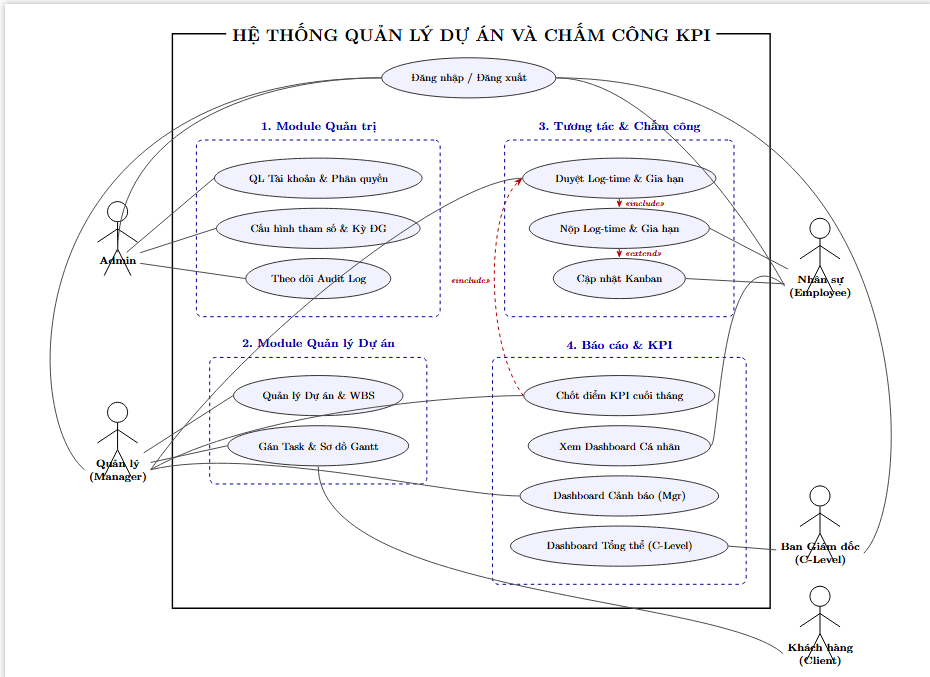
\includegraphics[width=0.95\textwidth]{uc_tong_quat_he_thong.png} % Thay bằng tên file ảnh của bạn
    \caption{Biểu đồ Use Case tổng quát của hệ thống quản lý dự án và chấm công KPI (Nguồn: Tác giả tự xây dựng)}
    \label{fig:uc_tong_quat_he_thong}
\end{figure}




Để đặc tả rõ hơn về logic vận hành bên trong của biểu đồ, phương pháp "Mô tả kịch bản Use Case" (Use Case Scenario Description) được áp dụng. Kịch bản này làm rõ tiền điều kiện, luồng sự kiện chính (Main Success Scenario) và kết quả đầu ra của các luồng nghiệp vụ quan trọng nhất. Dưới đây là đặc tả cho hai Use Case nền tảng: "Đăng nhập" (cửa ngõ bảo mật) và "Log-time giờ làm" (nguồn thu thập dữ liệu gốc).



\begin{table}[H]
    \centering
    \renewcommand{\arraystretch}{1.5}
    \begin{tabularx}{\textwidth}{|C{2.5cm}|X|X|}
    \hline
    \textbf{Tác nhân} & \multicolumn{1}{c|}{\textbf{Các bước thực hiện (Luồng sự kiện chính)}} & \multicolumn{1}{c|}{\textbf{Kết quả (Post-condition)}} \\
    \hline
    \textbf{Mọi người dùng} \newline \textit{(Use Case: Đăng nhập hệ thống)} & 
    1. Người dùng nhập thông tin (Email/Password) tại màn hình Đăng nhập. \newline 
    2. Frontend gửi request mã hóa lên Backend API. \newline 
    3. Backend đối chiếu cơ sở dữ liệu, xác thực mật khẩu qua thuật toán Hash. \newline 
    4. Nếu hợp lệ, hệ thống sinh ra một chuỗi JSON Web Token (JWT) chứa thông tin Role và gửi về Client. \newline 
    5. Frontend giải mã Token và điều hướng người dùng. & 
    Đăng nhập thành công. Người dùng được chuyển hướng vào giao diện \textit{Dashboard} tương ứng với phân quyền (Admin/Manager/Employee). Hệ thống khởi tạo phiên làm việc (\textit{Session}). \\
    \hline
    \textbf{Employee} \newline \textit{(Use Case: Log-time giờ làm)} & 
    1. Nhân sự chọn thẻ công việc (Task) đang ở trạng thái "Doing" trên bảng Kanban. \newline 
    2. Cập nhật trạng thái Task sang "Done". Hệ thống lập tức \textit{trigger} (kích hoạt) \textit{Form Log-time}. \newline 
    3. Nhân sự nhập số giờ làm việc thực tế (\textit{Actual Hours}) và chèn liên kết/tài liệu đính kèm làm minh chứng. \newline 
    4. Nhấn "Gửi phê duyệt". Hệ thống ghi nhận \textit{Timestamp} tại thời điểm gửi. & 
    Dữ liệu \textit{Log-time} được lưu vào Database với trạng thái "Pending" (Chờ duyệt). Hệ thống tự động đẩy thông báo (\textit{Notification}) đến tài khoản Manager quản lý trực tiếp dự án đó. \\
    \hline
    \end{tabularx}
    \caption{Mô tả kịch bản chi tiết cho các Use Case cốt lõi}
    \label{tab:usecase_scenarios}
\end{table}

\subsection{Yêu cầu chức năng và Phi chức năng (Bảo mật, Hiệu suất)}

\textbf{1. Yêu cầu chức năng (Functional Requirements)}
Dựa trên phân tích Use Case, hệ thống phải đáp ứng đầy đủ các chức năng vận hành cơ bản: 
Từ phía Admin, hệ thống yêu cầu các chức năng CRUD cho việc quản lý danh mục phòng ban, người dùng và tham số hệ thống. Từ phía Manager, hệ thống yêu cầu công cụ khởi tạo dự án, phân rã WBS, thiết lập sơ đồ Gantt, và chốt điểm số KPI. Từ phía Employee, hệ thống yêu cầu giao diện tương tác kéo-thả Kanban, chức năng cập nhật trạng thái và nộp Log-time.

\textbf{2. Yêu cầu phi chức năng (Non-Functional Requirements)}
Nếu yêu cầu chức năng định nghĩa "Hệ thống phải làm gì", thì yêu cầu phi chức năng (NFR) định nghĩa "Hệ thống phải làm điều đó tốt như thế nào". Đối với một hệ thống MIS doanh nghiệp, các tiêu chuẩn kiến trúc này mang tính chất quyết định:

\begin{itemize}
    \item \textbf{Yêu cầu về Bảo mật (Security):} Dữ liệu về giờ làm và điểm KPI liên quan trực tiếp đến chi phí và lương thưởng của doanh nghiệp, do đó tính bảo mật phải được đặt ở mức cao nhất. Hệ thống phải sử dụng chuẩn mã hóa mật khẩu (ví dụ: Bcrypt). Cơ chế xác thực và phân quyền phải được thực hiện thông qua JWT ở tầng Middleware của Backend (C\# .NET Core), chặn đứng mọi nỗ lực truy cập trái phép qua API (Bypass API). Mọi thao tác làm thay đổi dữ liệu đều phải được lưu vết trong bảng \textit{Audit Log} để phục vụ công tác thanh tra.
    
    \item \textbf{Yêu cầu về Hiệu suất (Performance):} Hệ thống phải đảm bảo xử lý mượt mà trong môi trường có tính đồng thời cao (Concurrency), đặc biệt là vào những ngày cuối tháng khi toàn bộ nhân sự cùng truy cập để nộp Log-time và Manager chốt KPI. Thời gian phản hồi (Response Time) của các API truy vấn thông thường phải dưới $500ms$. Các tác vụ nặng như quét cảnh báo trễ hạn hay tính toán điểm KPI hàng loạt không được làm nghẽn luồng xử lý chính (Main thread), mà phải được đẩy xuống chạy ngầm (Background Jobs) thông qua thư viện \textit{Hangfire}.
    
    \item \textbf{Yêu cầu về Tính khả dụng (Usability) và Trải nghiệm người dùng (UX):} Một hệ thống quản trị chỉ thành công khi người dùng không cảm thấy nó là một gánh nặng. Giao diện (Frontend) phải được phát triển bằng ReactJS với thiết kế \textit{Single Page Application (SPA)}, mang lại trải nghiệm thao tác mượt mà không cần tải lại trang. Chức năng cập nhật tiến độ (Kanban) phải hỗ trợ tính năng kéo-thả (Drag and Drop) trực quan. Thiết kế \textit{Dashboard} phải tuân thủ nguyên lý thị giác, sử dụng các dải màu (Xanh/Vàng/Đỏ) để làm nổi bật các cảnh báo rủi ro (Risk Alert) và tình trạng quá tải (Overload).
\end{itemize}

\section{Thiết kế Quy trình nghiệp vụ (Business Logic)} 
\subsection{Quy trình giao việc và quản lý tiến độ (WBS \& Kanban)}

Quy trình giao việc và quản lý tiến độ là luồng nghiệp vụ xương sống (Core Business Flow) của toàn bộ hệ thống MIS. Quá trình này không chỉ đơn thuần là việc phân công nhiệm vụ từ cấp trên xuống cấp dưới, mà là một chuỗi các thao tác logic được hệ thống kiểm soát chặt chẽ, trải dài từ khâu hoạch định cấu trúc phân rã công việc (WBS) cho đến khi trực quan hóa tiến trình thực thi trên bảng Kanban. Luồng hoạt động này được chia thành các giai đoạn thiết yếu sau:

\textbf{Giai đoạn 1: Hoạch định và Phân rã cấu trúc công việc (WBS)}
Quy trình bắt đầu khi Quản lý dự án (Manager) khởi tạo một không gian dự án mới. Tại giao diện lập kế hoạch, Manager tiến hành bóc tách dự án lớn thành các Gói công việc (Epics), Nhiệm vụ (Tasks) và Nhiệm vụ con (Sub-tasks) theo đúng chuẩn phương pháp luận WBS.
Mỗi một thẻ Task được tạo ra trên hệ thống yêu cầu cấu hình một bộ tham số ràng buộc bắt buộc, bao gồm: 
\begin{itemize}
    \item \textbf{Định danh và Mô tả:} Tên Task, nội dung chi tiết, và tài liệu đính kèm (nếu có).
    \item \textbf{Phân bổ nguồn lực:} Định danh tài khoản nhân sự chịu trách nhiệm chính (\textit{Assignee}). Hệ thống tự động kiểm tra xem nhân sự này có đang bị quá tải (\textit{Overload}) trong cùng khung thời gian hay không để đưa ra cảnh báo cho Manager.
    \item \textbf{Tham số thời gian:} Ngày bắt đầu (\textit{Start Date}), Hạn chót (\textit{Due Date}) và Số giờ nỗ lực dự kiến (\textit{Estimated Hours}). Các tham số này là cơ sở gốc để động cơ KPI tính toán tỷ lệ Hiệu suất sau này.
    \item \textbf{Thiết lập tính phụ thuộc (\textit{Task Dependencies}):} Manager phải xác định các Task tiền quyết (\textit{Predecessors}). Logic hệ thống được lập trình để ngăn chặn việc bắt đầu một Task nếu Task tiền quyết của nó chưa chuyển sang trạng thái hoàn thành (Áp dụng quan hệ Finish-to-Start).
\end{itemize}

\textbf{Giai đoạn 2: Ánh xạ dữ liệu và Khởi tạo Bảng Kanban}
Ngay sau khi Manager nhấn "Xác nhận giao việc", Backend API sẽ ghi nhận dữ liệu vào các bảng \texttt{Projects} và \texttt{Tasks} trong cơ sở dữ liệu SQL Server. Dựa trên trường \textit{Assignee\_ID}, hệ thống tự động phân phối và ánh xạ các tác vụ này lên giao diện không gian làm việc cá nhân của từng Employee.
Lúc này, trên giao diện Frontend (ReactJS), bảng Kanban của nhân sự sẽ tự động xuất hiện các thẻ Card tương ứng tại cột "Cần làm" (\textit{To Do}). Cơ chế này đảm bảo nhân sự chỉ nhìn thấy đúng phần việc của mình, tuân thủ nguyên tắc giới hạn hiển thị dữ liệu (\textit{Data Visibility}).

\textbf{Giai đoạn 3: Tương tác thực thi và Xử lý đồng bộ (Sync Processing)}
Trong quá trình làm việc, Employee thực hiện việc cập nhật tiến độ thông qua thao tác kéo-thả (\textit{Drag \& Drop}) thẻ Card từ cột \textit{To Do} sang \textit{Doing}, và cuối cùng là \textit{Done}. Đằng sau thao tác hình ảnh đơn giản này là một chuỗi xử lý kỹ thuật phức tạp:
Khi một thẻ bị thả vào cột mới, giao diện ReactJS sẽ bắt sự kiện (\textit{Event Listener}) và ngay lập tức gửi một \textit{HTTP PATCH Request} mang theo ID của Task và Trạng thái mới lên máy chủ .NET Core. Tại tầng Backend, hệ thống tiến hành ba bước xác thực: (1) Kiểm tra \textit{Token JWT} xem người dùng có đúng là \textit{Assignee} của Task này hay không; (2) Kiểm tra ràng buộc tiền quyết (Các Task phụ thuộc đã xong chưa); (3) Nếu hợp lệ, tiến hành cập nhật bản ghi trong cơ sở dữ liệu và ghi vết vào \textit{Audit Log}. Cuối cùng, Backend trả về phản hồi thành công (\textit{HTTP 200 OK}), lúc này thẻ trên bảng Kanban mới chính thức được cố định ở cột mới.

\textbf{Giai đoạn 4: Tự động hóa kiểm soát tiến độ (Cron Jobs)}
Hệ thống không phụ thuộc vào việc con người tự giác báo cáo trễ hạn. Bằng việc tích hợp thư viện \textit{Hangfire}, một luồng tác vụ chạy ngầm (\textit{Background Job}) được thiết lập để quét toàn bộ cơ sở dữ liệu mỗi 30 phút một lần. Thuật toán sẽ so sánh \textit{Due Date} của tất cả các Task đang ở cột \textit{To Do} và \textit{Doing} với \textit{Current System Time}. Nếu phát hiện quá hạn, hệ thống tự động cưỡng chế chuyển trạng thái thẻ Task đó sang cột \textit{Overdue} (Trễ hạn), đổi màu thẻ sang cảnh báo Đỏ trên giao diện Kanban, đồng thời kích hoạt chuông thông báo (\textit{Push Notification}) đến cả Employee và Manager quản lý trực tiếp. 

\begin{figure}[H]
    \centering
    \begin{tikzpicture}[
        box/.style={rectangle, draw=black, thick, fill=white, minimum width=2.4cm, minimum height=0.9cm, align=center, font=\scriptsize},
        decision/.style={diamond, draw=black, thick, fill=white, minimum width=0.8cm, minimum height=0.8cm, align=center, font=\tiny},
        line/.style={draw, thick, -{Stealth[scale=1.2]}},
        label/.style={font=\tiny\itshape}
    ]
        % Vẽ các đường phân làn (Swimlanes)
        \draw[dashed, gray] (-3, 1) -- (-3, -16.5);
        \draw[dashed, gray] (2.2, 1) -- (2.2, -16.5);
        
        % Tiêu đề các làn
        \node[font=\small\bfseries] at (-5.5, 0.7) {User (Emp / Mgr)};
        \node[font=\small\bfseries] at (-0.4, 0.7) {Frontend (ReactJS)};
        \node[font=\small\bfseries] at (5, 0.7) {Backend \& DB (.NET / SQL / Hangfire)};

        % --- GIAI ĐOẠN 1: WBS ---
        \node[circle, draw, fill=black, minimum size=0.4cm] (start1) at (-5.5, 0) {};
        \node[box] (act1) at (-5.5, -1.2) {\textnormal{Khởi tạo dự án} \\ \& \textnormal{Phân rã WBS}};
        \node[box] (act2) at (-0.4, -1.2) {\textnormal{Bắt sự kiện, gửi} \\ \textnormal{Request tạo Task}};
        \node[box] (act3) at (5, -1.2) {\textnormal{Lưu thông tin vào} \\ DB SQL Server};
        
        \path[line] (start1) -- (act1);
        \path[line] (act1) -- (act2);
        \path[line] (act2) -- (act3);

        % --- GIAI ĐOẠN 2: ÁNH XẠ KANBAN ---
        \node[box] (act4) at (5, -3) {\textnormal{Phân phối Task theo} \\ Assignee\_ID};
        \node[box] (act5) at (-0.4, -3) {\textnormal{Hiển thị thẻ tại} \\ \textnormal{cột To Do cá nhân}};
        
        \path[line] (act3) -- (act4);
        \path[line] (act4) -- (act5);

        % --- GIAI ĐOẠN 3: TƯƠNG TÁC THỰC THI ---
        \node[box] (act6) at (-5.5, -4.8) {Employee \textnormal{kéo thả} \\ \textnormal{thẻ sang Doing/Done}};
        \node[box] (act7) at (-0.4, -4.8) {\textnormal{Gửi} HTTP PATCH \\ Request (JWT Token)};
        \node[decision] (dec1) at (5, -4.8) {\textnormal{Xác thực} JWT \\ \& \textnormal{Task tiền quyết?}};
        
        \path[line] (act5) |- (act6);
        \path[line] (act6) -- (act7);
        \path[line] (act7) -- (dec1);

        % Nhánh rẽ Đúng / Sai của Giai đoạn 3 - ĐÃ HẠ KHỐI LỖI XUỐNG TOẠ ĐỘ TRỤC Y=-5.8 ĐỂ NÉ HÌNH THOI
        \node[box] (act8) at (5, -8.0) {\textnormal{Cập nhật trạng thái,} \\ \textnormal{ghi vết Audit Log}};
        \node[box] (act10) at (7.6, -5.8) {\textnormal{Trả lỗi} HTTP 400 \\/ 401}; 
        \node[box] (act11) at (-0.4, -5.8) {\textnormal{Trả thẻ về} \\ \textnormal{vị trí cũ}};
        \node[box] (act9) at (-0.4, -8.0) {\textnormal{Cố định thẻ tại} \\ \textnormal{cột mới (HTTP 200)}};

        \path[line] (dec1) -- node[label, left] {\textnormal{Đúng}} (act8);
        \path[line] (dec1) -| node[label, above, xshift=-1cm] {\textnormal{Sai}} (act10);
        \path[line] (act8) -- (act9);
        \path[line] (act10) -- (act11);

        % --- GIAI ĐOẠN 4: CRON JOBS HANGFIRE ---
        \node[circle, draw, fill=white, double=black, minimum size=0.4cm] (start2) at (5, -10.2) {};
        \node[box] (act12) at (5, -11.4) {Hangfire \textnormal{quét} DB \\ \textnormal{định kỳ mỗi 30 phút}};
        \node[decision] (dec2) at (5, -13.2) {\textnormal{Task trễ hạn} \\ (Due Date)?};
        \node[box] (act13) at (5, -15.0) {\textnormal{Cưỡng chế chuyển} \\ \textnormal{trạng thái Overdue}};
        \node[box] (act14) at (-0.4, -15.0) {\textnormal{Đổi thẻ màu Đỏ,} \\ \textnormal{kích hoạt chuông}};
        \node[box] (act15) at (-5.5, -15.0) {\textnormal{Nhận cảnh báo} \\ \textnormal{trễ hạn Real-time}};
        
        \node[circle, draw, double=black, fill=black, minimum size=0.4cm] (stop1) at (-5.5, -16.0) {};

        \path[line] (start2) -- (act12);
        \path[line] (act12) -- (dec2);
        \path[line] (dec2) -- node[label, left] {\textnormal{Có}} (act13);
        \path[line] (act13) -- (act14);
        \path[line] (act14) -- (act15);
        
        \path[line] (act15) -- (stop1);
        \path[line] (act9) |- (-2.5,-9.2) |- (stop1);
        \path[line] (act11) |- (-2.5,-6.3) |- (stop1);
        \draw[thick] (dec2.east) -- node[label, above] {\textnormal{Không}} ++(1,0) |- (5,-16.0) -- (stop1);
    \end{tikzpicture}
    \caption{Sơ đồ hoạt động (Activity Diagram) mô tả quy trình giao việc và quản lý tiến độ (Nguồn: Tác giả tự xây dựng)}
    \label{fig:activity_wbs_kanban}
\end{figure}

\subsection{Quy trình báo cáo giờ làm (Log-time) và Phê duyệt}

Dữ liệu thời gian làm việc thực tế (Log-time) là nguồn "nhiên liệu" thô quan trọng nhất quyết định đến tính chính xác của toàn bộ hệ thống đánh giá KPI. Nếu dữ liệu đầu vào bị sai lệch hoặc thao túng (Garbage In), mọi thuật toán tính toán phía sau đều trở nên vô nghĩa (Garbage Out). Do đó, quy trình báo cáo giờ làm và phê duyệt được thiết kế như một chốt chặn bảo vệ tính toàn vẹn dữ liệu (Data Integrity).

\textbf{1. Cơ chế Log-time và tính tất yếu của khâu Phê duyệt (Approval Workflow)}
Quy trình bắt đầu khi nhân sự (Employee) hoàn thành một gói công việc và kéo thẻ Task sang cột "Done" trên bảng Kanban. Lúc này, hệ thống sẽ thiết lập một \textit{Hard-constraint} (Ràng buộc cứng): Không cho phép đóng Task nếu nhân sự chưa hoàn thành \textit{Form Log-time}.
Tại biểu mẫu này, nhân sự phải điền chính xác số giờ đã tiêu hao (\textit{Actual Hours}) và đặc biệt bắt buộc phải cung cấp minh chứng (Ví dụ: Link GitHub commit, Link Google Drive chứa tài liệu báo cáo, hoặc ảnh chụp màn hình). Toàn bộ dữ liệu này sau khi \textit{Submit} sẽ được lưu vào cơ sở dữ liệu với trạng thái \textit{Pending} (Chờ duyệt).

Tại sao quy trình này bắt buộc phải có khâu phê duyệt từ Quản lý (Manager)? 
Trong môi trường thực tế, việc tự báo cáo (Self-reporting) luôn đi kèm với rủi ro thiên kiến chủ quan hoặc gian lận (nhân viên có xu hướng khai khống số giờ để tăng điểm hiệu suất). Khâu phê duyệt của Manager đóng vai trò là màng lọc kiểm chứng. Manager sẽ đối chiếu số giờ khai báo với chất lượng tài liệu minh chứng để quyết định \textit{Approve} (Duyệt) hoặc \textit{Reject} (Từ chối, yêu cầu làm lại). Chỉ những bản ghi Log-time có trạng thái \textit{Approved} mới được hệ thống truy xuất để đưa vào thuật toán tính KPI cuối tháng.

\textbf{2. Xử lý ách tắc luồng duyệt bằng Tự động hóa (Auto-Approve)}
Một nhược điểm chí mạng của luồng phê duyệt thủ công là rủi ro Quản lý "ngâm" hồ sơ, quên duyệt giờ làm, dẫn đến việc nhân sự không được tính lương. Để khắc phục, hệ thống tích hợp một tiến trình chạy ngầm (\textit{Background Job}) bằng thư viện \textit{Hangfire}. Luồng \textit{Cron Job} này sẽ liên tục quét các bản ghi \textit{Pending}. Nếu một yêu cầu Log-time không được Manager xử lý sau 48 giờ (hoặc trước ngày chốt công 24 giờ), hệ thống sẽ gửi Email cảnh báo tối hậu thư. Hết hạn cảnh báo, hệ thống tự động chuyển trạng thái bản ghi sang \textit{Auto-Approved}. Cơ chế này giải quyết triệt để nút thắt cổ chai trong quy trình, bảo vệ tuyệt đối quyền lợi của người lao động.

\subsection{Động cơ tính toán KPI tự động và Xử lý ngoại lệ}

"Động cơ tính toán KPI" (KPI Engine) là phân hệ phức tạp nhất, đóng vai trò là bộ não phân tích của toàn bộ nền tảng MIS. Thay vì tính toán rải rác, KPI Engine được thiết kế để chạy theo cơ chế xử lý lô (\textit{Batch Processing}) vào ngày cuối cùng của kỳ đánh giá (ví dụ: ngày 30 hàng tháng) nhằm tối ưu hóa tài nguyên máy chủ.

\textbf{1. Công thức tính toán tổng quát}
Hệ thống loại bỏ hoàn toàn các đánh giá cảm tính bằng cách định lượng hóa hiệu suất thông qua 4 trụ cột cơ bản, được cấu hình với các trọng số (\textit{Weight}) mặc định như sau:
\begin{itemize}
    \item \textbf{Tiến độ ($P_1$ - 40\%):} $P_1 = (\text{Số Task Done đúng hạn} / \text{Tổng số Task}) \times 100$.
    \item \textbf{Hiệu suất ($P_2$ - 30\%):} $P_2 = (\text{Tổng Estimated Hours} / \text{Tổng Actual Hours}) \times 100$. (Giới hạn trần ở mức $120\%$ để tránh các trường hợp ước lượng sai lệch quá lớn).
    \item \textbf{Khối lượng ($P_3$ - 20\%):} $P_3 = (\text{Tổng Actual Hours} / \text{Số giờ làm chuẩn trong tháng}) \times 100$.
    \item \textbf{Điểm chất lượng ($P_4$ - 10\%):} Điểm do Manager đánh giá trực tiếp dựa trên thái độ và mức độ hỗ trợ đồng đội.
\end{itemize}

Công thức tổng hợp cuối cùng:
$$KPI_{\text{Tổng}} = (P_1 \times 0.4) + (P_2 \times 0.3) + (P_3 \times 0.2) + (P_4 \times 0.1)$$

\begin{figure}[H]
    \centering
    \begin{tikzpicture}[
        box/.style={rectangle, draw=black, thick, fill=white, minimum width=3.2cm, minimum height=0.9cm, align=center, font=\scriptsize},
        decision/.style={diamond, draw=black, thick, fill=white, minimum width=1cm, minimum height=1cm, align=center, font=\tiny},
        line/.style={draw, thick, -{Stealth[scale=1.2]}},
        label/.style={font=\tiny\itshape}
    ]
        % --- VẾ TRÁI: ĐI TỪ TRÊN XUỐNG ---
        \node[circle, draw, fill=black, minimum size=0.4cm] (start) at (0,0) {};
        
        \node[box] (act1) at (0, -1.2) {
            \textnormal{Kích hoạt Batch Job} \\ 
            \textnormal{(Cuối ngày 30 hàng tháng)}
        };
        
        \node[box] (act2) at (0, -2.8) {
            \textnormal{Quét danh sách nhân sự} \\ 
            \textnormal{từ bảng Employee}
        };
        
        \node[box] (act3) at (0, -4.4) {
            \textnormal{Lấy các bản ghi Log-time} \\ 
            \textnormal{có trạng thái "Approved"}
        };
        
        \node[box] (act4) at (0, -6.0) {
            \textnormal{Tính P1 (Tiến độ), P3 (Khối lượng)} \\ 
            \textnormal{và lấy P4 (Điểm chất lượng)}
        };
        
        \node[box] (act5) at (0, -7.6) {
            \textnormal{Tính toán Hiệu suất thô} \\ 
            $P_2 = \frac{\text{Est Hours}}{\text{Actual Hours}} \times 100$
        };
        
        \node[decision] (dec1) at (0, -9.5) {$P_2 > 120\%$?};
        
        \node[box] (act6) at (0, -11.4) {
            \textnormal{Giới hạn trần} \\ 
            $P_2 = 120\%$
        };

        % --- BẺ LUỒNG SANG PHẢI VÀ ĐI NGƯỢC LÊN (VẾ PHẢI) ---
        \node[box] (act7) at (5, -11.4) {
            \textnormal{Áp dụng trọng số cấu hình} \\ 
            \textnormal{(40\%, 30\%, 20\%, 10\%)}
        };
        
        \node[box] (act8) at (5, -7.6) {
            \textnormal{Tổng hợp điểm KPI cuối cùng} \\ 
            \textnormal{theo công thức tổng quát}
        };
        
        \node[box] (act9) at (5, -4.4) {
            \textnormal{Lưu bản ghi kết quả} \\ 
            \textnormal{vào bảng KPI\_Reports}
        };
        
        \node[decision] (dec2) at (5, -2.0) {
            \textnormal{Hết danh sách} \\ 
            \textnormal{nhân sự?}
        };
        
        \node[circle, draw, double=black, fill=black, minimum size=0.4cm] (stop) at (5, 0) {};

        % --- KẾT NỐI LUỒNG MŨI TÊN CHUẨN ĐÃ ÉP CỐ ĐỊNH HƯỚNG ---
        % Vế trái đi xuống tuần tự
        \path[line] (start) -- (act1);
        \path[line] (act1) -- (act2);
        \path[line] (act2) -- (act3);
        \path[line] (act3) -- (act4);
        \path[line] (act4) -- (act5);
        \path[line] (act5) -- (dec1);
        \path[line] (dec1) -- node[label, left] {\textnormal{Có}} (act6);
        
        % Kết nối vế trái sang vế phải ở đáy chữ U
        \path[line] (act6) -- (act7);
        \path[line] (dec1.east) -- node[label, above] {\textnormal{Không}} ++(1.5,0) |- (act7.west);
        
        % ÉP ĐẦU MŨI TÊN CHỈ THẲNG LÊN TRỜI (SỬA LỖI NGƯỢC HÌNH)
        \path[line] (act7.north) -- (act8.south);
        \path[line] (act8.north) -- (act9.south);
        \path[line] (act9.north) -- (dec2.south);
        \path[line] (dec2.north) -- node[label, left] {\textnormal{Đúng}} (stop);
        
        % Vòng lặp đóng quay ngược lại khối quét nhân sự (act2) từ phải sang trái
        \path[line] (dec2.west) -- node[label, above] {\textnormal{Sai}} (act2.east);
        
    \end{tikzpicture}
    \caption{Lưu đồ thuật toán tối ưu của Động cơ tính toán KPI (KPI Engine) (Nguồn: Tác giả tự xây dựng)}
    \label{fig:kpi_engine_flowchart}
\end{figure}


\textbf{2. Các cơ chế xử lý ngoại lệ (Exception Handling)}
Một thuật toán tính điểm cứng nhắc sẽ làm hỏng văn hóa doanh nghiệp. Do đó, KPI Engine được lập trình để nhận diện và xử lý các kịch bản ngoại lệ trong luồng nghiệp vụ thực tế, đảm bảo sự nhân văn và tính toàn vẹn của hệ thống phần mềm.



\begin{table}[H]
    \centering
    \renewcommand{\arraystretch}{1.5}
    \begin{tabularx}{\textwidth}{|C{3.5cm}|C{4cm}|X|}
    \hline
    \textbf{Tình huống ngoại lệ} & \textbf{Dấu hiệu nhận biết (\textit{Trigger Condition})} & \multicolumn{1}{c|}{\textbf{Cơ chế xử lý của hệ thống (\textit{System Handling})}} \\
    \hline
    \textbf{Nhân sự quá tải (Overload)} & Tỷ lệ Khối lượng ($P_3$) vượt quá $110\%$ NHƯNG tỷ lệ Tiến độ ($P_1$) vẫn đạt từ $90\%$ trở lên. & Thuật toán tự động kích hoạt "Hệ số vượt khó". Tổng điểm KPI cuối cùng sẽ được nhân thêm hệ số thưởng $1.1$ ($+10\%$ tổng điểm) nhằm ghi nhận nỗ lực gánh vác dự án. \\
    \hline
    \textbf{Trễ hạn có cảnh báo rủi ro sớm (Risk Alert)} & Task bị trễ hạn (\textit{Overdue}) nhưng nhân sự đã bật cờ "Cảnh báo rủi ro" trước hạn chót ít nhất 48 giờ. & Hệ thống hiển thị \textit{Flag} (Cờ) trên màn hình chốt KPI của Manager. Manager có quyền click "Miễn trừ hình phạt", hệ thống sẽ không tính Task này vào tỷ lệ trễ hạn khi tính $P_1$. \\
    \hline
    \textbf{Lỗi chia cho 0 (Division by Zero)} & Mẫu số trong các công thức $P_1, P_2, P_3$ bằng $0$ (Xảy ra khi nhân sự mới vào làm, chưa được gán Task nào hoặc chưa có Log-time). & Bắt lỗi \textit{Exception} ở tầng Backend. Hệ thống tự động gán giá trị KPI của tiêu chí đó bằng $0\%$ hoặc \textit{N/A} để tránh làm sập (\textit{Crash}) toàn bộ tiến trình quét KPI của công ty. \\
    \hline
    \end{tabularx}
    \caption{Các loại ngoại lệ nghiệp vụ và cơ chế xử lý tự động của KPI Engine}
    \label{tab:kpi_exceptions}
\end{table}


\section{Thiết kế Cơ sở dữ liệu và Giao diện}
\subsection{Sơ đồ thực thể liên kết (ERD Diagram)}

Thiết kế cơ sở dữ liệu quan hệ (Relational Database Design) là nền tảng kỹ thuật tối quan trọng nhằm đảm bảo tính toàn vẹn dữ liệu, tối ưu hóa tốc độ truy vấn và ngăn chặn các dị thường dữ liệu (Anomalies) trong quá trình thêm, sửa, xóa. Hệ thống thông tin quản lý này được thiết kế tuân thủ nghiêm ngặt dạng chuẩn 3 (Third Normal Form - 3NF). Cấu trúc dữ liệu trung tâm của hệ thống được xây dựng dựa trên sự tương tác logic giữa 5 thực thể cốt lõi sau:

\begin{itemize}
    \item \textbf{Thực thể Người dùng (User):} Lưu trữ toàn bộ thông tin định danh và tài khoản của nhân sự trong tổ chức. Thực thể này có mối quan hệ nhiều-một (N-1) với các thực thể \textit{Role} và \textit{Department} để thiết lập cơ chế phân quyền RBAC và giới hạn hiển thị dữ liệu theo phòng ban.
    \item \textbf{Thực thể Dự án (Project):} Đại diện cho các dự án tổng thể do doanh nghiệp triển khai. Thực thể này lưu trữ các thông tin vĩ mô như tên dự án, mã dự án, ngày bắt đầu, hạn chót và trạng thái hiện tại. Mỗi dự án sẽ có một mối quan hệ một-nhiều (1-N) với thực thể \textit{Task} (một dự án bao hàm nhiều công việc được phân rã).
    \item \textbf{Thực thể Công việc (Task):} Trọng tâm của cấu trúc phân rã công việc (WBS). Thực thể này không chỉ lưu trữ thông tin về nội dung công việc, nhân sự được gán (\textit{AssigneeId}), số giờ dự kiến (\textit{EstimatedHours}) mà còn chứa mối quan hệ đệ quy (Self-referencing Relationship) thông qua khóa ngoại \textit{ParentTaskId} để biểu diễn cấu trúc cây đa cấp độ của WBS. Đồng thời, mối quan hệ nhiều-nhiều (N-N) giữa các Task độc lập được cấu trúc qua bảng trung gian để thể hiện tính phụ thuộc (\textit{Task Dependencies}).
    \item \textbf{Thực thể Ghi nhận Giờ làm (LogTime):} Thực thể động, liên tục phát sinh bản ghi khi nhân sự cập nhật tiến độ công việc. Mỗi bản ghi \textit{LogTime} liên kết chặt chẽ với một \textit{Task} (quan hệ N-1) và một \textit{User} tạo lập (quan hệ N-1). Thực thể này bắt buộc phải lưu trữ trường dữ liệu chứng cứ (\textit{EvidenceUrl}) và trạng thái phê duyệt của Quản lý.
    \item \textbf{Thực thể Hiệu suất (KPI):} Lưu trữ kết quả điểm số đã chốt của nhân sự theo từng kỳ đánh giá tháng. Nhằm tối ưu hóa hiệu năng và tránh việc máy chủ phải tính toán lại các công thức toán học phức tạp mỗi khi tải trang Dashboard, thực thể này được thiết kế để lưu trữ dữ liệu tĩnh sau khi động cơ KPI Engine chạy xử lý lô (\textit{Batch Processing}) vào cuối tháng.
\end{itemize}

Kiến trúc lưu trữ và mối tương quan giữa các thực thể dữ liệu cốt lõi trong hệ thống quản lý thông tin dự án và đánh giá KPI tự động được đặc tả thông qua Sơ đồ thực thể mối quan hệ (Entity Relationship Diagram - ERD) tại Hình \ref{fig:ERD_DB}.

\begin{figure}[H]
    \centering
    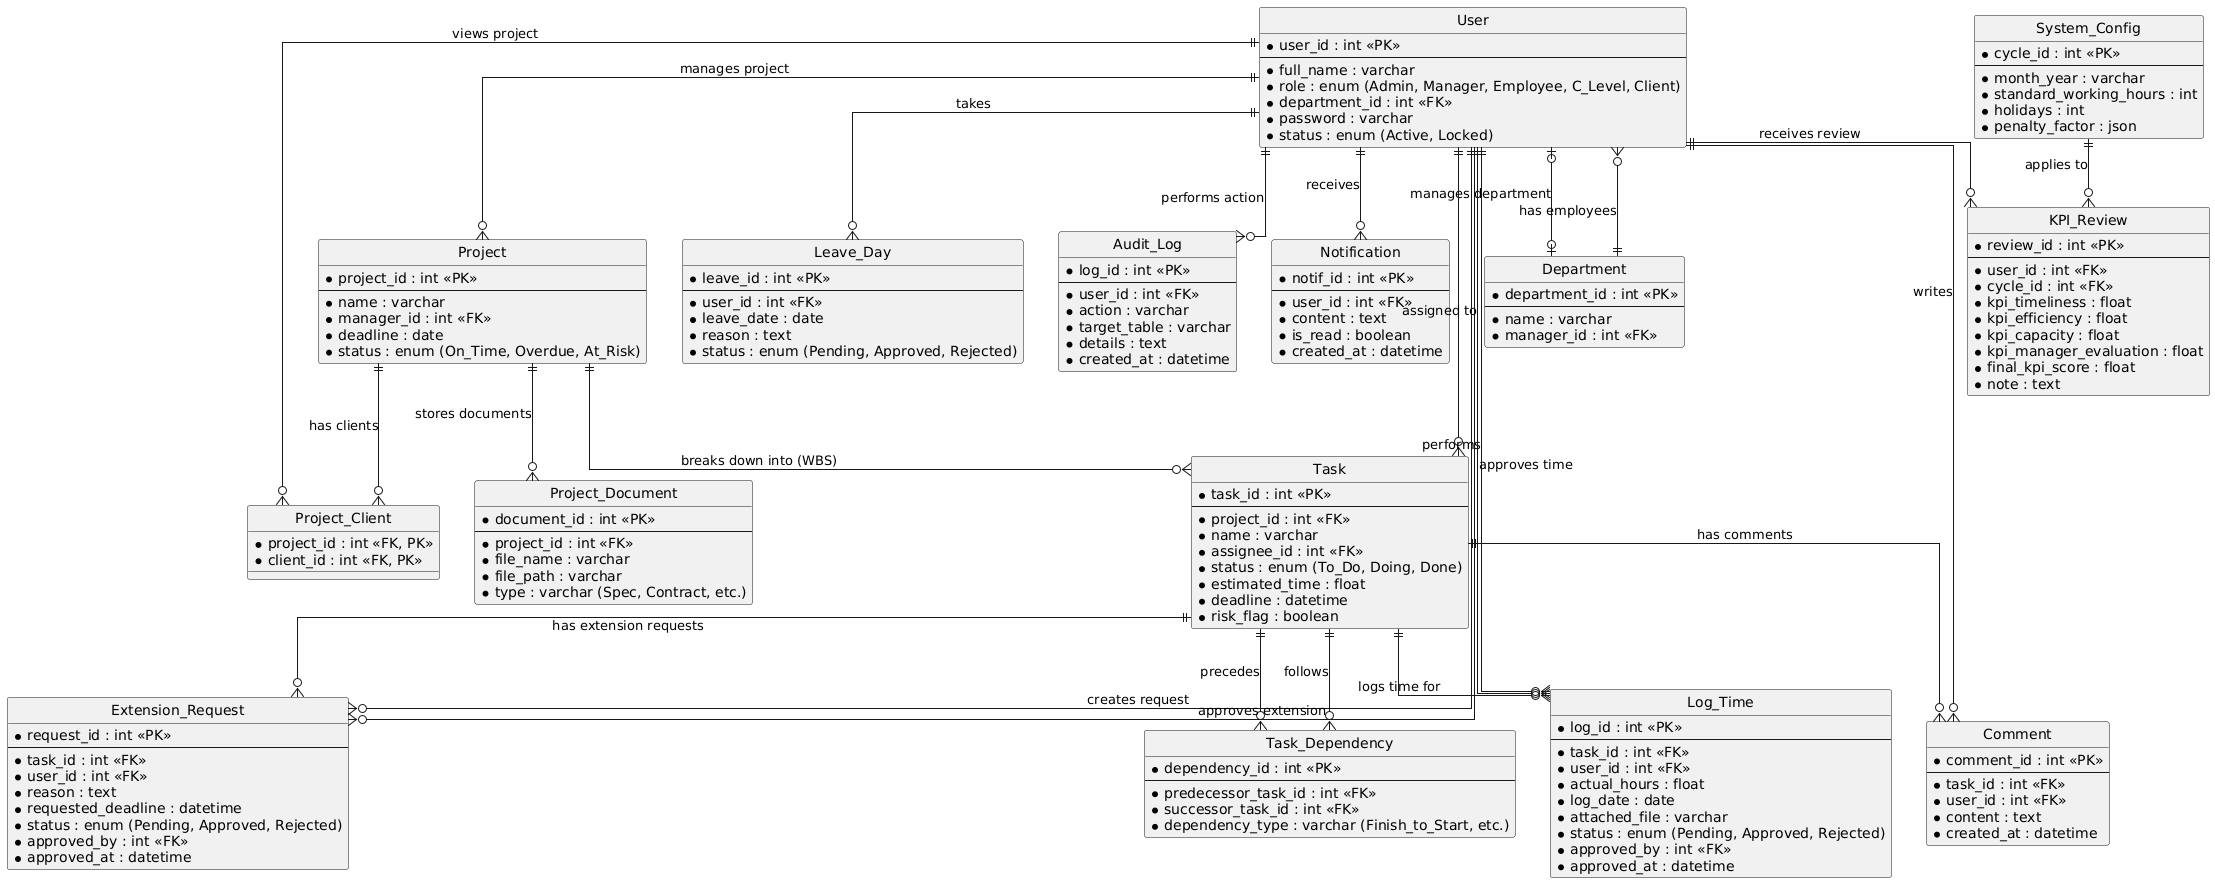
\includegraphics[width=0.95\textwidth]{ERD_DB.png} % Hãy lưu ảnh ERD của bạn với tên mis-erd.png rồi upload lên Overleaf
    \caption{Sơ đồ thực thể mối quan hệ (ERD) của hệ thống quản lý dự án và KPI (Nguồn: Tác giả tự xây dựng)}
    \label{fig:ERD_DB}
\end{figure}


\subsection{Cấu trúc các bảng dữ liệu cốt lõi (Data Dictionary)}

Để chuyển đổi sơ đồ thực thể liên kết (ERD) lý thuyết thành kiến trúc vật lý trên hệ quản trị cơ sở dữ liệu Microsoft SQL Server, việc xây dựng Từ điển dữ liệu (Data Dictionary) là bắt buộc. Dưới đây là đặc tả chi tiết về kiểu dữ liệu, ràng buộc khóa chính (PK), khóa ngoại (FK) và thuộc tính của 3 bảng dữ liệu quan trọng nhất hệ thống.



\begin{table}[H]
    \centering
    \renewcommand{\arraystretch}{1.5}
    \begin{tabularx}{\textwidth}{|C{3.5cm}|C{3.5cm}|X|}
    \hline
    \textbf{Tên trường (Field)} & \textbf{Kiểu dữ liệu (Type)} & \multicolumn{1}{c|}{\textbf{Mô tả và Ràng buộc}} \\
    \hline
    \texttt{UserId} & \texttt{INT (Identity)} & Khóa chính (Primary Key), tự động tăng, định danh duy nhất người dùng. \\
    \hline
    \texttt{Username} & \texttt{VARCHAR(50)} & Tên đăng nhập hệ thống, thuộc tính duy nhất (\textit{Unique}), không được để trống. \\
    \hline
    \texttt{PasswordHash} & \texttt{VARCHAR(255)} & Chuỗi mật khẩu đã qua mã hóa một chiều bằng thuật toán \textit{BCrypt}, bảo mật tầng DB. \\
    \hline
    \texttt{Email} & \texttt{VARCHAR(100)} & Email công vụ của nhân sự, dùng để gửi thông báo tự động và xác thực. \\
    \hline
    \texttt{RoleId} & \texttt{INT} & Khóa ngoại (Foreign Key) liên kết với bảng \texttt{Roles} để phân quyền truy cập API. \\
    \hline
    \texttt{DepartmentId} & \texttt{INT} & Khóa ngoại (Foreign Key) liên kết với bảng \texttt{Departments} để phân nhóm bộ phận. \\
    \hline
    \texttt{CreatedAt} & \texttt{DATETIME} & Thời gian khởi tạo tài khoản trên hệ thống, mặc định lấy \textit{GETDATE()}. \\
    \hline
    \end{tabularx}
    \caption{Từ điển dữ liệu bảng Người dùng (Users Table)}
    \label{tab:dict_users}
\end{table}



\begin{table}[H]
    \centering
    \renewcommand{\arraystretch}{1.5}
    \begin{tabularx}{\textwidth}{|C{3.5cm}|C{3.5cm}|X|}
    \hline
    \textbf{Tên trường (Field)} & \textbf{Kiểu dữ liệu (Type)} & \multicolumn{1}{c|}{\textbf{Mô tả và Ràng buộc}} \\
    \hline
    \texttt{TaskId} & \texttt{INT (Identity)} & Khóa chính (Primary Key), định danh duy nhất của mỗi nhiệm vụ/công việc. \\
    \hline
    \texttt{ProjectId} & \texttt{INT} & Khóa ngoại (Foreign Key), liên kết với bảng \texttt{Projects} để xác định thuộc dự án nào. \\
    \hline
    \texttt{TaskName} & \texttt{NVARCHAR(150)} & Tên của công việc, sử dụng Unicode hỗ trợ tiếng Việt, không được để trống. \\
    \hline
    \texttt{AssigneeId} & \texttt{INT} & Khóa ngoại (Foreign Key), liên kết với bảng \texttt{Users}, xác định nhân sự chịu trách nhiệm. \\
    \hline
    \texttt{EstimatedHours} & \texttt{DECIMAL(5,2)} & Số giờ công nỗ lực dự kiến được Quản lý phê duyệt khi bóc tách WBS. \\
    \hline
    \texttt{StartDate} & \texttt{DATETIME} & Ngày bắt đầu triển khai công việc theo kế hoạch. \\
    \hline
    \texttt{DueDate} & \texttt{DATETIME} & Hạn chót phải hoàn thành công việc để tránh rơi vào trạng thái \textit{Overdue}. \\
    \hline
    \texttt{Status} & \texttt{VARCHAR(20)} & Trạng thái trên bảng Kanban: \textit{'To Do', 'Doing', 'Done', 'Overdue'}. \\
    \hline
    \texttt{ParentTaskId} & \texttt{INT (Nullable)} & Khóa ngoại tự liên kết (Self-FK) dùng để phân rã Task thành các Sub-task đa tầng. \\
    \hline
    \end{tabularx}
    \caption{Từ điển dữ liệu bảng Công việc (Tasks Table)}
    \label{tab:dict_tasks}
\end{table}



\begin{table}[H]
    \centering
    \renewcommand{\arraystretch}{1.5}
    \begin{tabularx}{\textwidth}{|C{3.5cm}|C{3.5cm}|X|}
    \hline
    \textbf{Tên trường (Field)} & \textbf{Kiểu dữ liệu (Type)} & \multicolumn{1}{c|}{\textbf{Mô tả và Ràng buộc}} \\
    \hline
    \texttt{LogTimeId} & \texttt{INT (Identity)} & Khóa chính (Primary Key), định danh duy nhất của mỗi bản ghi khai báo giờ làm. \\
    \hline
    \texttt{TaskId} & \texttt{INT} & Khóa ngoại (Foreign Key), liên kết trực tiếp với bảng \texttt{Tasks} được chấm công. \\
    \hline
    \texttt{UserId} & \texttt{INT} & Khóa ngoại (Foreign Key), liên kết với bảng \texttt{Users} để xác định người khai báo. \\
    \hline
    \texttt{ActualHours} & \texttt{DECIMAL(4,2)} & Số giờ làm việc thực tế mà nhân sự tiêu hao cho công việc đó. \\
    \hline
    \texttt{EvidenceUrl} & \texttt{VARCHAR(500)} & Đường dẫn liên kết chứa minh chứng kỹ thuật (Link GitHub, Tài liệu, Hình ảnh đầu ra). \\
    \hline
    \texttt{ApprovalStatus} & \texttt{VARCHAR(20)} & Trạng thái luồng duyệt: \textit{'Pending', 'Approved', 'Rejected', 'AutoApproved'}. \\
    \hline
    \texttt{ApprovedById} & \texttt{INT (Nullable)} & Khóa ngoại, liên kết với bảng \texttt{Users}, xác định tài khoản Manager đã thực hiện duyệt. \\
    \hline
    \texttt{SubmittedAt} & \texttt{DATETIME} & Mốc thời gian hệ thống ghi nhận khi nhân sự bấm nút gửi yêu cầu phê duyệt. \\
    \hline
    \end{tabularx}
    \caption{Từ điển dữ liệu bảng Báo cáo giờ làm (LogTime Table)}
    \label{tab:dict_logtime}
\end{table}
\subsection{Thiết kế Wireframe và hệ thống Dashboards (UI/UX)}

Thiết kế giao diện người dùng (User Interface - UI) và trải nghiệm người dùng (User Experience - UX) trong một hệ thống thông tin quản lý (MIS) không chỉ dừng lại ở bài toán thẩm mỹ đồ họa, mà đóng vai trò là "giao lộ" trung gian chuyển hóa cấu trúc dữ liệu phức tạp ở tầng Backend thành các tri thức vận hành trực quan. Đối với "Hệ thống thông tin quản lý tiến độ công việc và đánh giá KPI tự động", cấu trúc giao diện được xây dựng nghiêm ngặt dựa trên triết lý Thiết kế lấy người dùng làm trung tâm (User-Centered Design - UCD) và nguyên tắc phân quyền đa vai trò (Role-based UI Kit). 

Tư duy thiết kế này đòi hỏi mọi thành phần giao diện phải được tinh chỉnh dựa trên đặc thù hành vi và nhu cầu tiêu thụ thông tin của từng nhóm tác nhân hệ thống (Personas). Hệ thống được phân rã thành các phân hệ giao diện trực quan độc lập bao gồm:

\begin{itemize}
    \item \textbf{Phân hệ tương tác Nhân sự (Employee Portal):} Giao diện tối giản, tập trung hiển thị trực quan các thanh tiến độ đo lường KPI cá nhân theo thời gian thực (Tiến độ, Hiệu suất, Khối lượng, Điểm quản lý), danh sách các tác vụ sắp đến hạn (\textit{Due Soon}), và bảng kéo thả Kanban hỗ trợ nhân viên cập nhật trạng thái công việc nhanh chóng dưới 3 cú click chuột.
    
    \item \textbf{Phân hệ Điều hành Quản lý (Manager \& MIS Dashboard):} Chuyển dịch sang mô hình "Trung tâm điều hành" để trực quan hóa dữ liệu tổng thể của toàn dự án. Phân hệ cung cấp các bảng cảnh báo rủi ro tải lượng nhân sự (\textit{Overload Heatmap}), sơ đồ tiến độ tổng thể (\textit{Gantt Overview}), trung tâm phê duyệt Timesheet/Log-time tập trung, và bảng tổng hợp chốt điểm KPI tự động cho toàn bộ nhân sự vào cuối kỳ đánh giá.
    
    \item \textbf{Phân hệ Quản trị hệ thống (Admin Console):} Cung cấp các biểu mẫu tối giản phục vụ cho công tác xác thực, quản trị danh mục dữ liệu (\textit{CRUD tài khoản, phân quyền, gán phòng ban}), thiết lập linh hoạt các tham số cấu hình hệ thống ngầm (\textit{Số ngày làm việc chuẩn, hệ số phạt trễ hạn}), và giám sát an toàn thông tin thông qua bảng nhật ký vết thao tác (\textit{Audit Log}).
\end{itemize}

Để minh họa cho cấu trúc trải nghiệm người dùng trước khi tiến hành lập trình giao diện Front-end, kiến trúc phân tầng UI/UX được định hình thông qua các bản vẽ sơ đồ khung xương chức năng (Wireframe) chi tiết cho từng phân hệ từ Hình \ref{fig:wf_emp} đến Hình \ref{fig:wf_mis_reports}.

% --- BỘ ẢNH WIREFRAME ---
\begin{figure}[H]
    \centering
    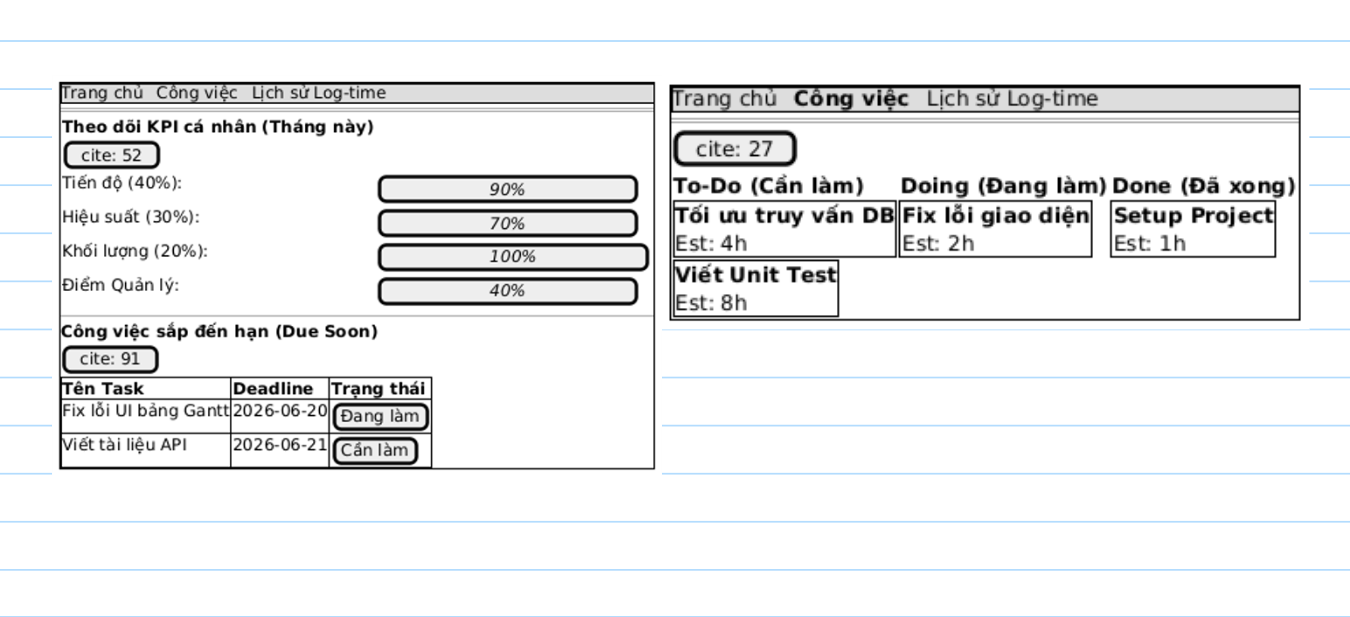
\includegraphics[width=0.85\textwidth]{employee-dashboard.png}
    \caption{Wireframe giao diện Trang chủ Nhân sự và không gian làm việc Kanban (Nguồn: Tác giả tự thiết kế)}
    \label{fig:wf_emp}
\end{figure}

\begin{figure}[H]
    \centering
    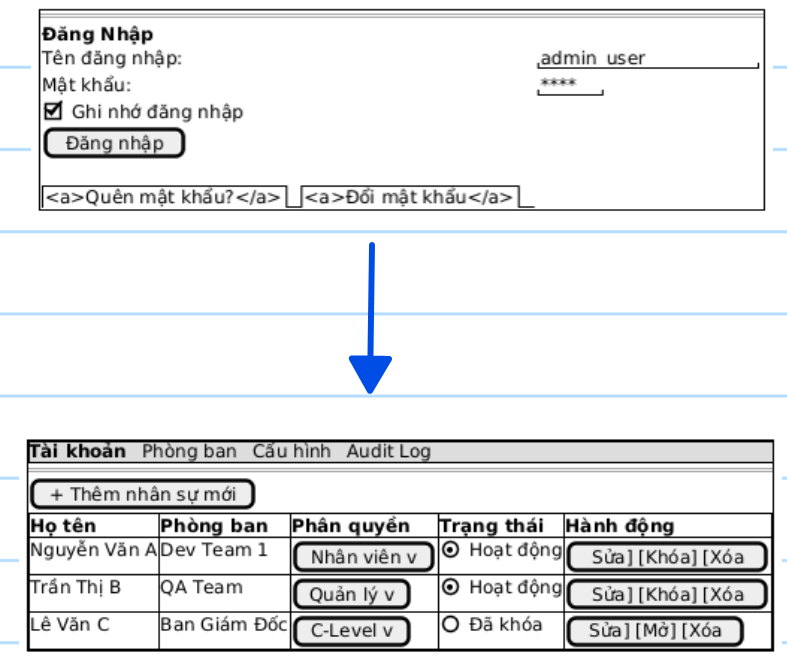
\includegraphics[width=0.85\textwidth]{admin-portal.png}
    \caption{Wireframe giao diện cổng Đăng nhập và phân hệ CRUD tài khoản của Admin (Nguồn: Tác giả tự thiết kế)}
    \label{fig:wf_admin}
\end{figure}

\begin{figure}[H]
    \centering
    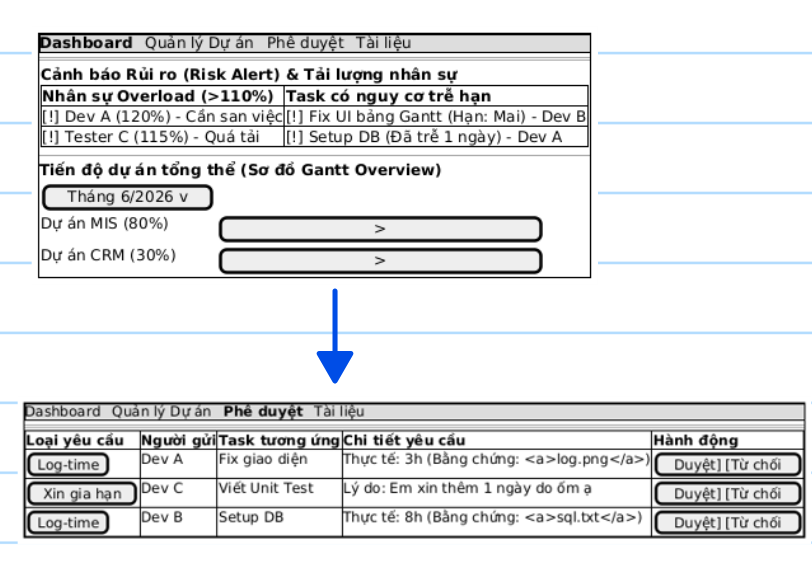
\includegraphics[width=0.85\textwidth]{manager-dashboard.png}
    \caption{Wireframe giao diện Trang chủ Quản lý và Trung tâm phê duyệt Log-time (Nguồn: Tác giả tự thiết kế)}
    \label{fig:wf_manager}
\end{figure}

\begin{figure}[H]
    \centering
    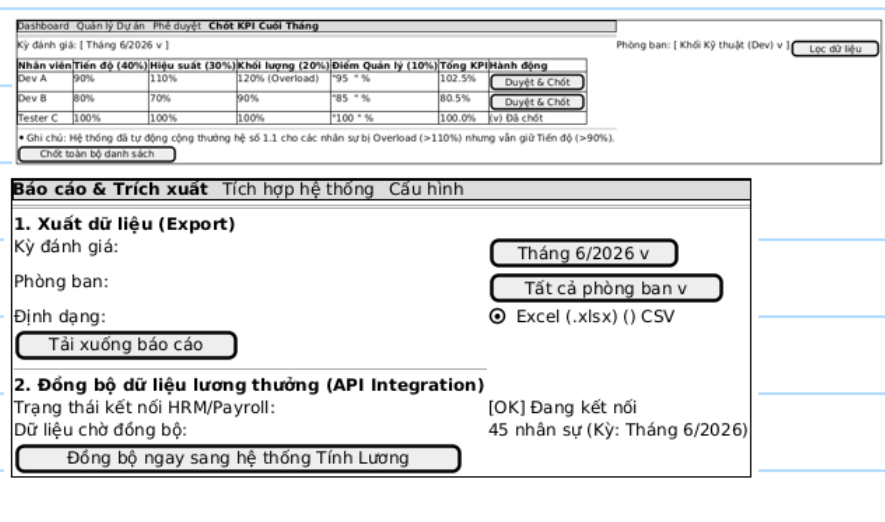
\includegraphics[width=0.85\textwidth]{mis-kpi-reports.png}
    \caption{Wireframe giao diện Bảng đánh giá chốt điểm KPI và trích xuất dữ liệu tích hợp (Nguồn: Tác giả tự thiết kế)}
    \label{fig:wf_mis_reports}
\end{figure}

Dựa trên sơ đồ kiến trúc Wireframe phân vai trò tổng quan, toàn bộ hệ thống Web Application được phân rã thành một danh mục các màn hình chức năng cụ thể. Bảng \ref{tab:ui_screens_list} dưới đây đặc tả chi tiết mục tiêu tương tác và cấu phần giao diện thực tế của nền tảng.

\begin{table}[H]
    \centering
    \renewcommand{\arraystretch}{1.5}
    \begin{tabularx}{\textwidth}{|c|C{3.5cm}|C{2.5cm}|X|}
    \hline
    \textbf{STT} & \textbf{Tên màn hình} & \textbf{Tác nhân chính} & \multicolumn{1}{|c|}{\textbf{Mục tiêu tương tác \& Cấu phần cốt lõi}} \\
    \hline
    1 & Màn hình Đăng nhập (Auth Portal) & Mọi tác nhân & Xác thực danh tính thông qua giao diện tối giản. Hệ thống tự động điều hướng luồng giao diện dựa trên Role được giải mã từ Token JWT. \\
    \hline
    2 & Không gian làm việc Dự án (Project Workspace) & Manager, Employee & Hiển thị thanh đo lường chỉ số KPI cá nhân, danh sách Task sắp đến hạn và bảng kéo thả Kanban hỗ trợ thao tác cập nhật tiến độ cho nhân viên. \\
    \hline
    3 & Trung tâm Phê duyệt một cửa (Approval Center) & Manager & Giao diện xử lý tập trung luồng dữ liệu Timesheet. Cho phép lọc nhanh các yêu cầu Log-time trạng thái \textit{Pending}, hiển thị URL minh chứng để Manager nhấn Duyệt/Từ chối hàng loạt. \\
    \hline
    4 & Bảng cấu hình Hệ thống (Admin Settings) & Admin & Giao diện CRUD tài khoản người dùng, phân bổ phòng ban và cập nhật các tham số cấu hình ngầm như định mức số ngày làm việc chuẩn, hệ số phạt trễ hạn. \\
    \hline
    5 & Tổng đàn Hiệu suất (MIS Dashboard) & Manager, C-Level & Hiển thị các chỉ số đồ họa: Cảnh báo quá tải (\textit{Overload}), sơ đồ tiến độ Gantt Overview, bảng đánh giá chốt KPI cuối tháng và phân hệ trích xuất báo cáo đồng bộ HRM. \\
    \hline
    \end{tabularx}
    \caption{Danh mục các màn hình chức năng và mục tiêu tương tác UI/UX thực tế}
    \label{tab:ui_screens_list}
\end{table}
 

% --- CHƯƠNG 3 ---
\chapter{XÂY DỰNG, ÁP DỤNG VÀ TRIỂN KHAI HỆ THỐNG}

\section{Môi trường phát triển và Kiến trúc công nghệ}
\subsection{Môi trường cơ sở dữ liệu (Microsoft SQL Server)}

Trong kiến trúc tổng thể của Hệ thống thông tin quản lý (MIS) tiến độ công việc và đánh giá KPI tự động, phân hệ cơ sở dữ liệu đóng vai trò là nền tảng hạ tầng lưu trữ trung tâm, quyết định trực tiếp đến tính ổn định, tốc độ xử lý và độ an toàn của toàn bộ luồng thông tin doanh nghiệp. Hệ quản trị cơ sở dữ liệu quan hệ Microsoft SQL Server (MSSQL) đã được lựa chọn để triển khai thực tế vật lý cho hệ thống nhờ đáp ứng xuất sắc các tiêu chuẩn kỹ thuật khắt khe sau:

\textbf{1. Đảm bảo tính toàn vẹn dữ liệu tuyệt đối (Data Integrity):} 
Đặc thù của hệ thống MIS quản lý nhân sự và chấm công đòi hỏi dữ liệu phải tuân thủ nghiêm ngặt các thuộc tính ACID (Atomicity, Consistency, Isolation, Durability). MSSQL cung cấp cơ chế kiểm soát giao dịch (Transaction Management) mạnh mẽ, giúp ngăn chặn hoàn toàn hiện tượng xung đột dữ liệu khi nhiều nhân sự cùng tiến hành kéo thả Kanban hoặc nộp Log-time đồng thời tại một thời điểm. Các ràng buộc toàn vẹn (Integrity Constraints) như Khóa chính (Primary Key), Khóa ngoại (Foreign Key), và các quy tắc xóa tháp dòng (Cascade Deletes) được thiết lập chặt chẽ ở tầng cơ sở dữ liệu, ngăn ngừa triệt để hiện tượng "dữ liệu mồ côi" (Orphaned Data) – ví dụ: đảm bảo một bản ghi \texttt{LogTime} không thể tồn tại nếu tác vụ \texttt{Task} liên kết với nó bị xóa bỏ khỏi hệ thống.

\textbf{2. Tối ưu hóa năng lực xử lý truy vấn của động cơ KPI Engine:} 
Động cơ tính toán KPI cuối tháng vận hành theo cơ chế xử lý lô (\textit{Batch Processing}) trên một khối lượng dữ liệu cực kỳ khổng lồ, bao gồm hàng nghìn bản ghi Timesheet, lịch sử thay đổi thẻ công việc và cơ cấu phòng ban. Các thuật toán này đòi hỏi các phép nối đa bảng phức tạp (Complex Joins), các hàm gộp (Aggregation Functions) và hàm cửa sổ (\textit{Window Functions} như \texttt{SUM() OVER}, \texttt{ROW\_NUMBER()}). Đặc biệt, cấu trúc phân rã công việc đa cấp độ của WBS bắt buộc hệ thống phải thực hiện các truy vấn đệ quy sâu. Bộ tối ưu hóa truy vấn (\textit{Query Optimizer}) và tính năng Biểu thức bảng chung đệ quy (Recursive Common Table Expressions - CTE) của MSSQL cho phép tính toán và xây dựng các kế hoạch thực thi (\textit{Execution Plans}) thông minh, giúp giảm thiểu tối đa thời gian quét đĩa từ và phản hồi API trong vòng dưới 500ms.

\textbf{3. Cơ chế bảo mật và phân quyền tầng sâu:} 
MSSQL cung cấp các giải pháp bảo mật nâng cao như mã hóa dữ liệu trong suốt (Transparent Data Encryption - TDE) và bảo mật mức dòng (Row-Level Security - RLS). Tiêu chuẩn này giúp hệ thống MIS cấu trúc được quyền xem dữ liệu tĩnh: nhân viên chỉ được quyền truy cập vào các dòng dữ liệu KPI của chính bản thân họ, trong khi Manager có quyền xem toàn bộ dữ liệu thuộc phòng ban do mình quản lý, chặn đứng hoàn toàn các nguy cơ rò rỉ thông tin nội bộ từ tầng cơ sở dữ liệu.

% --- ĐOẠN CHÈN ẢNH SCREENSHOT SSMS ĐÃ ĐƯỢC CHUẨN HÓA ---
\begin{figure}[H]
    \centering
    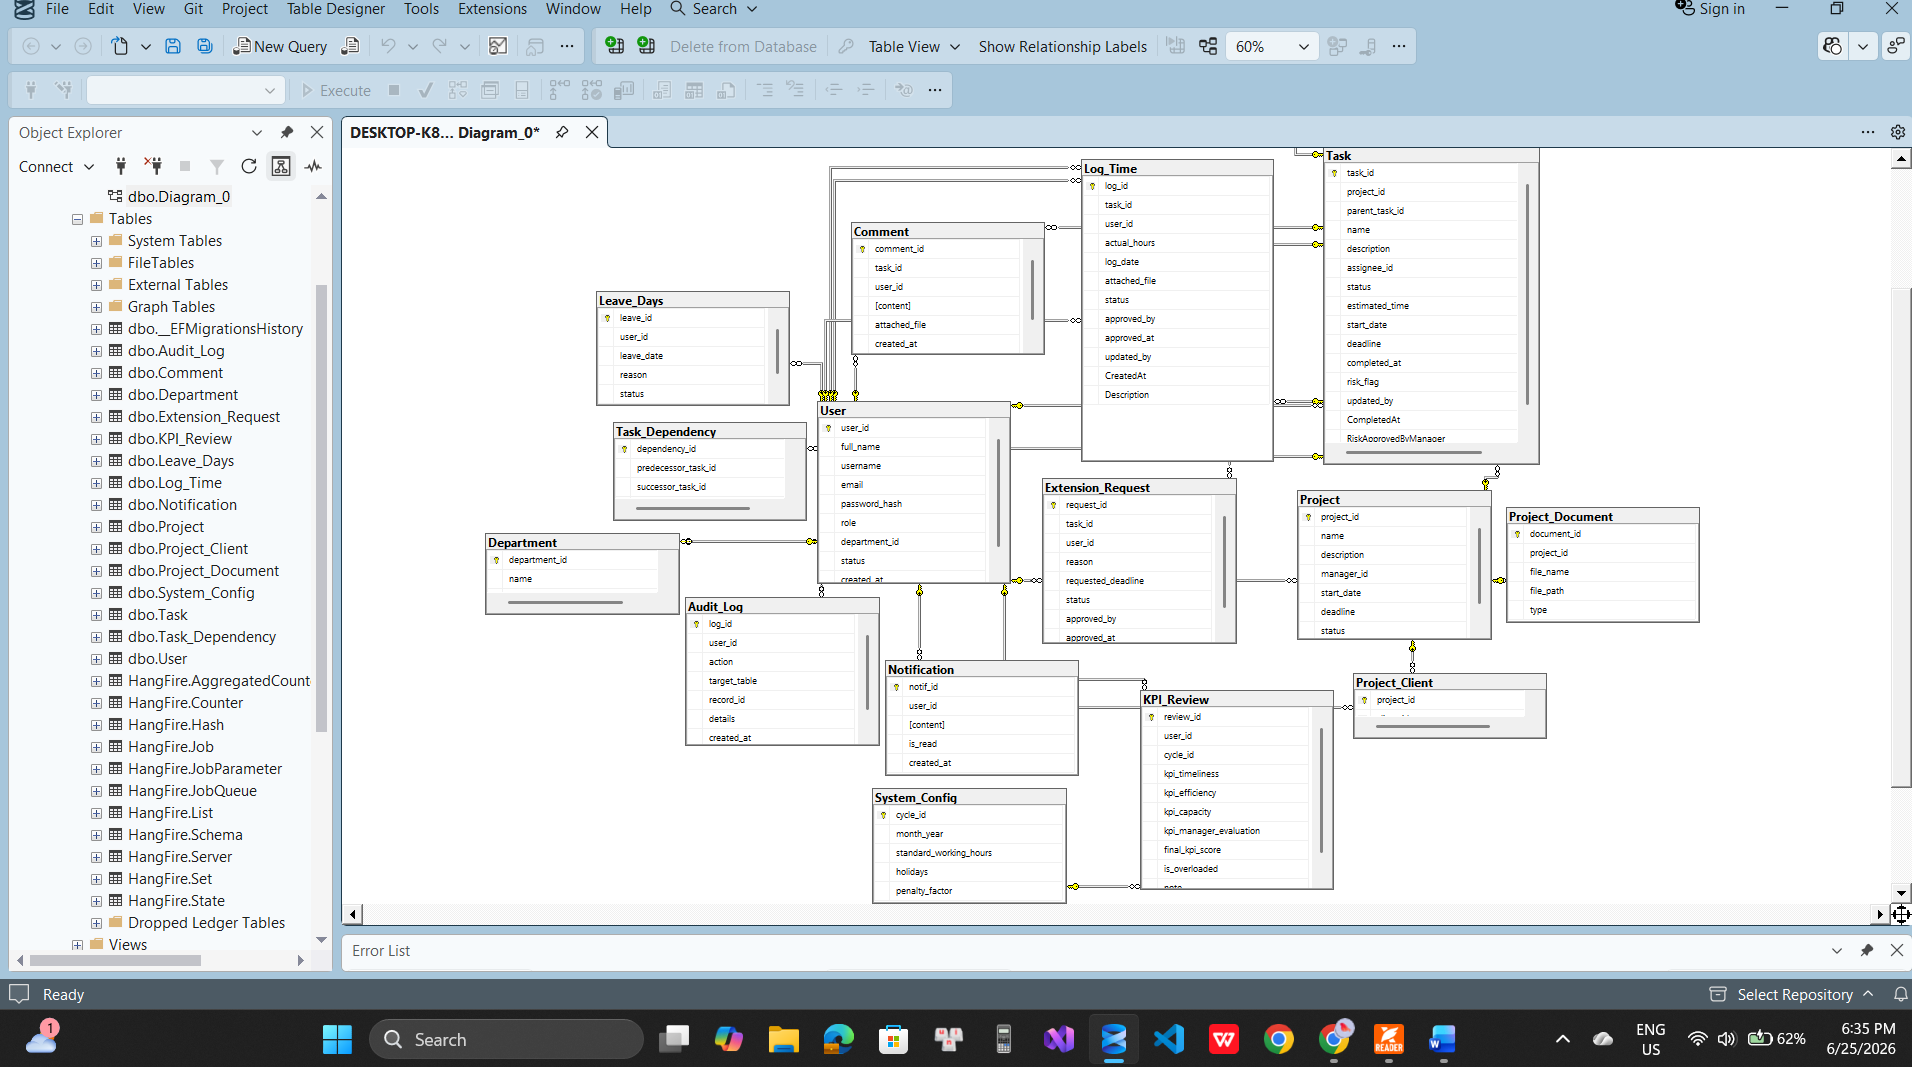
\includegraphics[width=0.9\textwidth]{trien_khai_SQL.png} % Thay bằng tên file ảnh chụp giao diện SQL của bạn
    \caption{Giao diện cấu trúc vật lý các bảng dữ liệu trên Microsoft SQL Server Management Studio (SSMS) (Nguồn: Tác giả tự chụp màn hình)}
    \label{fig:trien_khai_SQL}
\end{figure}

\textbf{4. Thiết lập môi trường kết nối và Chuỗi kết nối an toàn (Secure Connection String)}

Để kết nối giữa ứng dụng máy chủ Back-end (.NET Core) và Microsoft SQL Server, hệ thống áp dụng trình điều khiển \texttt{Microsoft.Data.SqlClient}. Nhằm tuân thủ nguyên tắc bảo mật thông tin, chuỗi kết nối kết nối tuyệt đối không được ghi mã cứng (Hard-code) vào trong các file mã nguồn nguồn để tránh lỗ hổng lộ lọt tài khoản khi đẩy mã nguồn lên các nền tảng quản lý mã nguồn tập trung (như GitHub). 

Trong môi trường phát triển (Development), chuỗi kết nối được lưu trữ mã hóa bằng công cụ \textit{User Secrets} của .NET Core. Khi triển khai lên môi trường thực tế (Production), chuỗi kết nối được cấu hình thông qua biến môi trường (Environment Variables) của hệ điều hành máy chủ với cấu trúc an toàn được định nghĩa như sau:

\begin{verbatim}
"ConnectionStrings": {
  "DefaultConnection": "Server=tcp:sqlserver-mis-kpi.database.windows.net,1433;
  Initial Catalog=MIS_KPI_DB;Persist Security Info=False;
  User ID=mis_api_user;Password={Secure_Password_Here};
  MultipleActiveResultSets=True;Encrypt=True;
  TrustServerCertificate=False;Connection Timeout=30;"
}
\end{verbatim}

Các tham số trong chuỗi kết nối trên được cấu hình nhằm tối ưu hóa tính phi chức năng của hệ thống phần mềm:
\begin{itemize}
    \item \texttt{Encrypt=True} và \texttt{TrustServerCertificate=False}: Bắt buộc toàn bộ lưu lượng dữ liệu truyền tải qua lại giữa Web Server (.NET Core API) và Database Server phải được mã hóa bằng giao thức SSL/TLS, ngăn chặn các cuộc tấn công nghe lén hoặc đánh cắp gói tin giữa đường (Man-in-the-middle Attack).
    \item \texttt{MultipleActiveResultSets=True} (MARS): Cho phép thực thi nhiều lô truy vấn đồng thời trên một kết nối duy nhất, một tính năng cực kỳ quan trọng giúp luồng chạy ngầm của \textit{Hangfire} có thể vừa đọc dữ liệu Log-time vừa ghi dữ liệu KPI vào bảng mà không gây ra tình trạng nghẽn kết nối (\textit{Connection Blocking}).
    \item \texttt{Connection Timeout=30}: Giới hạn thời gian chờ kết nối là 30 giây để giải phóng tài nguyên máy chủ ngay lập tức nếu xảy ra sự cố nghẽn mạng ngoại vi.
\end{itemize}

\subsection{Phát triển Backend API (.NET Core, Entity Framework)}

Trong kiến trúc Client-Server hiện đại của hệ thống thông tin quản lý (MIS), phân hệ Backend đóng vai trò là "bộ não" trung tâm, chịu trách nhiệm xử lý toàn bộ logic nghiệp vụ, xác thực phân quyền và giao tiếp với cơ sở dữ liệu. Nền tảng \textbf{.NET Core} (phiên bản mới nhất) được lựa chọn làm công cụ phát triển cốt lõi nhờ tính đa nền tảng (Cross-platform), hiệu năng xử lý cực cao và hệ sinh thái thư viện phong phú, đáp ứng hoàn hảo các tiêu chuẩn khắt khe của một hệ thống doanh nghiệp (Enterprise-level System).

\textbf{1. Ưu điểm của kiến trúc RESTful API trên nền tảng .NET Core}

Hệ thống được thiết kế theo chuẩn kiến trúc \textbf{RESTful API} (Representational State Transfer). Việc ứng dụng kiến trúc này trên .NET Core mang lại những ưu điểm vượt trội:
\begin{itemize}
    \item \textbf{Tính phi trạng thái (Statelessness):} Mỗi một HTTP Request từ phía Client (ReactJS) gửi lên Server đều độc lập và chứa đầy đủ thông tin (chủ yếu qua chuỗi JSON Web Token - JWT) để Server có thể xác thực và xử lý. Điều này giúp giảm tải bộ nhớ cho máy chủ vì không cần duy trì Session, tạo tiền đề để hệ thống dễ dàng mở rộng theo chiều ngang (Horizontal Scaling) khi số lượng nhân sự và dự án tăng vọt.
    \item \textbf{Cơ chế tiêm phụ thuộc (Dependency Injection - DI):} .NET Core cung cấp sẵn một bộ chứa IoC (Inversion of Control Container) mạnh mẽ. Việc áp dụng DI giúp giải quyết triệt để sự phụ thuộc cứng (Tight-coupling) giữa các module. Các thành phần như \textit{TaskService}, \textit{LogTimeService} hay \textit{EmailService} được tiêm vào các \textit{Controller} thông qua giao diện (Interface), giúp mã nguồn dễ dàng thực hiện kiểm thử đơn vị (Unit Testing) và bảo trì trong tương lai.
    \item \textbf{Xử lý bất đồng bộ (Asynchronous Programming):} Toàn bộ các luồng I/O-bound (như gọi Database hay gửi Email) đều được thiết kế theo cơ chế \textit{async/await}. Khi một luồng yêu cầu truy xuất cơ sở dữ liệu, luồng (Thread) của CPU sẽ không bị khóa (Non-blocking) mà được giải phóng để phục vụ các Request khác, giúp tăng thông lượng (Throughput) tối đa cho hệ thống vào những ngày cao điểm chốt KPI.
\end{itemize}

Toàn bộ chuỗi hành trình của một yêu cầu HTTP, từ lúc được kích hoạt tại giao diện Client cho đến khi đi qua các tầng xử lý logic của Back-end và tương tác với cơ sở dữ liệu thông qua Entity Framework Core được trực quan hóa chi tiết tại Hình \ref{fig:net_core_flow_chuandat}.

\begin{figure}[H]
    \centering
    \begin{tikzpicture}[
        box/.style={rectangle, draw=black, thick, fill=white, minimum width=2.8cm, minimum height=1.1cm, align=center, font=\scriptsize},
        line/.style={draw, thick, -{Stealth[scale=1.2]}},
        label/.style={font=\tiny\itshape}
    ]
        % Khai báo các khối kiến trúc chạy theo hàng ngang
        \node[box] (client) at (0,0) {Client Portal\\(ReactJS Web)};
        \node[box] (controller) at (4.2,0) {API Controllers\\(Routing \& JWT Auth)};
        \node[box] (service) at (8.4,0) {Business Services\\(\textnormal{Logic Nghiệp vụ})};
        \node[box] (efcore) at (12.6,0) {Entity Framework\\Core (ORM Layer)};
        \node[box, fill=gray!10] (db) at (12.6,-2.4) {Database Server\\(MS SQL Server)};

        % Mũi tên luồng đi xuôi (HTTP Request)
        \path[line] ([yshift=2.2mm]client.east) -- node[above, font=\tiny] {HTTP Request} ([yshift=2.2mm]controller.west);
        \path[line] ([yshift=2.2mm]controller.east) -- node[above, font=\tiny] {Call Service} ([yshift=2.2mm]service.west);
        \path[line] ([yshift=2.2mm]service.east) -- node[above, font=\tiny] {LINQ Query} ([yshift=2.2mm]efcore.west);
        \path[line] ([xshift=-2.5mm]efcore.south) -- node[left, font=\tiny] {SQL T-Code} ([xshift=-2.5mm]db.north);

        % Mũi tên luồng hồi đáp ngược lại (HTTP Response)
        \path[line] ([xshift=2.5mm]db.north) -- node[right, font=\tiny] {Raw Data} ([xshift=2.5mm]efcore.south);
        \path[line] ([yshift=-2.2mm]efcore.west) -- node[below, font=\tiny] {Entities} ([yshift=-2.2mm]service.east);
        \path[line] ([yshift=-2.2mm]service.west) -- node[below, font=\tiny] {DTO Objects} ([yshift=-2.2mm]controller.east);
        \path[line] ([yshift=-2.2mm]controller.west) -- node[below, font=\tiny] {JSON Response} ([yshift=-2.2mm]client.east);
        
    \end{tikzpicture}
    \caption{Sơ đồ luồng xử lý tuần tự kiến trúc RESTful API và EF Core trên nền tảng .NET Core (Nguồn: Tác giả tự xây dựng)}
    \label{fig:net_core_flow_chuandat}
\end{figure}


\textbf{2. Tối ưu hóa tương tác dữ liệu với Entity Framework Core}

Để giao tiếp với Microsoft SQL Server, hệ thống sử dụng \textbf{Entity Framework Core (EF Core)} - một công cụ ánh xạ đối tượng quan hệ (Object-Relational Mapping - ORM) toàn diện. EF Core loại bỏ hoàn toàn việc phải viết các câu lệnh SQL thuần túy (Raw SQL) dài dòng và tiềm ẩn rủi ro bảo mật.
\begin{itemize}
    \item \textbf{Truy vấn an toàn với LINQ (Language Integrated Query):} Lập trình viên có thể truy vấn cơ sở dữ liệu trực tiếp bằng cú pháp C\# strongly-typed. Quá trình biên dịch sẽ tự động kiểm tra lỗi cú pháp, đồng thời cơ chế tham số hóa (Parameterization) tự động của LINQ giúp hệ thống miễn nhiễm hoàn toàn với các cuộc tấn công \textit{SQL Injection}.
    \item \textbf{Quản lý phiên bản Database qua Migrations:} Phương pháp \textit{Code-First} được áp dụng. Mọi thay đổi về cấu trúc bảng (thêm trường mới, đổi kiểu dữ liệu) đều được định nghĩa thông qua các lớp Thực thể (Entity Classes) bằng C\#. Công cụ Migrations của EF Core sẽ tự động biên dịch các thay đổi này thành mã SQL tương ứng và cập nhật vào Database, giúp đội ngũ phát triển dễ dàng kiểm soát phiên bản (Version Control) của cơ sở dữ liệu cùng với mã nguồn.
\end{itemize}

\textbf{3. Mã nguồn C\# minh họa luồng xử lý truy xuất dữ liệu}

Dưới đây là một đoạn mã nguồn minh họa cách EF Core và LINQ được sử dụng để truy vấn danh sách các công việc (\textit{Tasks}) được gán cho một nhân sự (\textit{Employee}) cụ thể, bao gồm cả việc tải kèm dữ liệu dự án (Eager Loading) và tối ưu hóa bộ nhớ.

\begin{verbatim}
public async Task<IEnumerable<TaskDto>> GetTasksByUserIdAsync(int userId)
{
    // Truy vấn danh sách Task thông qua Entity Framework Core
    var tasks = await _dbContext.Tasks
        // Vô hiệu hóa cơ chế theo dõi sự thay đổi (Tracking) để tăng tốc độ truy vấn đọc
        .AsNoTracking()
        // Eager Loading: Tải kèm thông tin Dự án và Trạng thái liên quan
        .Include(t => t.Project)
        .Include(t => t.StatusCategory)
        // Điều kiện lọc LINQ: Chỉ lấy các công việc được gán cho User cụ thể
        .Where(t => t.AssigneeId == userId && t.IsDeleted == false)
        // Sắp xếp ưu tiên các công việc có hạn chót gần nhất
        .OrderBy(t => t.DueDate)
        // Thực thi truy vấn bất đồng bộ không chặn luồng (Non-blocking)
        .ToListAsync();

    // Sử dụng AutoMapper để ánh xạ từ Entity sang Data Transfer Object (DTO)
    // nhằm che giấu cấu trúc DB thật và tối ưu dung lượng JSON trả về
    return _mapper.Map<IEnumerable<TaskDto>>(tasks);
}
\end{verbatim}

\textbf{Giải thích logic mã nguồn:} 
Đoạn mã trên thể hiện rõ tính ưu việt của EF Core. Hàm \texttt{AsNoTracking()} là một kỹ thuật tối ưu hóa bộ nhớ cực kỳ quan trọng đối với các luồng \textit{GET API} chỉ đọc dữ liệu, giúp giảm tải công việc cho bộ thu gom rác (Garbage Collector). Hàm \texttt{Include()} giải quyết bài toán \textit{N+1 Query}, gộp các lần gọi dữ liệu liên quan thành một câu lệnh \texttt{JOIN} duy nhất dưới tầng SQL Server. Cuối cùng, hàm \texttt{ToListAsync()} đẩy tác vụ I/O xuống phần cứng, giải phóng luồng CPU hiện tại của .NET Core để đón nhận các HTTP Request khác của hệ thống.
\subsection{Phát triển Frontend (ReactJS) và Tự động hóa ngầm (Background Jobs - Hangfire)}

Để kiến tạo một Hệ thống thông tin quản lý (MIS) toàn diện, sức mạnh xử lý dữ liệu ở tầng Backend phải được song hành cùng một trải nghiệm giao diện mượt mà ở tầng Frontend và cơ chế vận hành bền bỉ ở tầng nền (Background). Việc kết hợp thư viện ReactJS cho giao diện người dùng và Hangfire cho các tác vụ chạy ngầm là một thiết kế kiến trúc mang tính chiến lược, giải quyết triệt để bài toán về tải trọng (Load) và trải nghiệm (UX).

\textbf{1. Kiến trúc Single Page Application (SPA) của ReactJS tối ưu hóa UI/UX}

Khác với các kiến trúc Web truyền thống (Multi-Page Application) yêu cầu trình duyệt phải tải lại toàn bộ trang (Full-page Reload) mỗi khi có tương tác, phân hệ Frontend của hệ thống được phát triển theo kiến trúc Ứng dụng trang đơn (Single Page Application - SPA) dựa trên thư viện \textbf{ReactJS}. 

Trong kiến trúc SPA, máy chủ chỉ trả về một tệp HTML duy nhất trong lần truy cập đầu tiên. Mọi thao tác chuyển trang, lọc dữ liệu hay cập nhật Bảng điều khiển (Dashboard) sau đó đều được thực hiện thông qua các lệnh gọi API bất đồng bộ (AJAX/Fetch) và JavaScript sẽ tự động vẽ lại (Render) các phần tử cần thiết trên màn hình. Đối với một hệ thống MIS đặc thù như quản lý dự án, kiến trúc SPA của ReactJS mang lại ba đột phá về mặt UX/UI:
\begin{itemize}
    \item \textbf{Tối ưu hóa thao tác kéo thả (Drag \& Drop):} Trên bảng Kanban, khi nhân sự kéo một thẻ công việc (Task) từ cột "Doing" sang "Done", cơ chế DOM Ảo (Virtual DOM) của ReactJS cho phép giao diện phản hồi ngay lập tức (Instant Feedback) bằng cách cập nhật State cục bộ, trong khi tiến trình gọi API lưu dữ liệu vào Backend vẫn đang chạy ngầm. Điều này xóa bỏ hoàn toàn độ trễ (Latency), mang lại cảm giác mượt mà như một ứng dụng Native trên Desktop.
    \item \textbf{Cấu trúc Component tái sử dụng (Component-based Architecture):} Các thành phần phức tạp trên hệ thống như Biểu đồ vành khăn (Donut Chart) tiến độ, Sơ đồ Gantt, hay các Form khai báo Log-time được chia nhỏ thành các Component độc lập. Việc đóng gói này giúp mã nguồn Frontend dễ dàng bảo trì và tái sử dụng ở nhiều màn hình Dashboard khác nhau (của Admin, Manager và Employee) mà không gây phình to dung lượng bộ nhớ.
    \item \textbf{Đồng bộ State toàn cục (Global State Management):} Sử dụng các công cụ quản lý trạng thái, khi Manager duyệt một yêu cầu Log-time ở phân hệ "Phê duyệt", dữ liệu tổng giờ làm trên "Dashboard Tiến độ" ở một trang khác sẽ lập tức được cập nhật theo thời gian thực (Real-time reactivity) mà không cần người dùng phải bấm nút tải lại trang (\textit{Refresh}).
\end{itemize}

Để minh họa cho mô hình tối ưu hóa UI/UX này, kiến trúc phân rã cấu phần và cơ chế đồng bộ mượt mà của Virtual DOM trên giao diện Kanban được trực quan hóa chi tiết tại Hình \ref{fig:react_vdom_flow}.

\begin{figure}[H]
    \centering
    \begin{tikzpicture}[
        box/.style={rectangle, draw=black, thick, fill=white, minimum width=2.8cm, minimum height=1.1cm, align=center, font=\scriptsize},
        line/.style={draw, thick, -{Stealth[scale=1.2]}},
        label/.style={font=\tiny\itshape}
    ]
        % Định vị các khối thành phần hệ thống chạy theo hàng ngang
        \node[box] (action) at (0,0) {\textnormal{Thao tác kéo thả} \\ \textnormal{(User Drag \& Drop)}};
        \node[box] (state) at (4.2,0) {\textnormal{Cập nhật State} \\ (Kanban Task State)};
        \node[box] (vdom) at (8.4,0) {Virtual DOM\\(\textnormal{Tính toán Diffing})};
        \node[box] (rdom) at (12.6,0) {Real DOM\\(\textnormal{UI Kanban mới})};

        % Thay thế đoạn kết nối mũi tên cũ bằng đoạn mã đã bẻ dòng chữ dưới đây:
        \path[line] (action) -- node[above, font=\tiny] {\textnormal{Trigger Event}} (state);
        \path[line] (state) -- node[above, font=\tiny, align=center] {Re-render\\Component} (vdom);
        \path[line] (vdom) -- node[above, font=\tiny] {Reconciliation} (rdom);
 

        % Đường phản hồi ngược mô tả vòng lặp UI mượt mà, không gây đóng băng ứng dụng
        \draw[thick, ->] (rdom.south) |- ++(-6.3,-0.9) -| node[below, font=\tiny, pos=0.25] {\textnormal{Phản hồi lập tức (Instant Feedback) -- Hoàn toàn không tải lại toàn bộ trang}} (action.south);
        
    \end{tikzpicture}
    \caption{Sơ đồ luồng dữ liệu và cơ chế đồng bộ Virtual DOM trong phân hệ bảng Kanban (Nguồn: Tác giả tự xây dựng)}
    \label{fig:react_vdom_flow}
\end{figure}


\textbf{2. Vai trò của Hangfire trong tự động hóa và xử lý tác vụ ngầm}

Một trong những sai lầm thiết kế (\textit{Anti-pattern}) nguy hiểm nhất trong các hệ thống Web là thực thi các tác vụ tính toán nặng (Heavy Computing) đồng bộ trên luồng chính (\textit{Main Request Pipeline}). Ví dụ, nếu Manager nhấn nút "Chốt KPI toàn công ty", hệ thống phải quét hàng nghìn bản ghi Log-time, tính toán các công thức phức tạp và ghi vào Database. Nếu chạy đồng bộ, luồng xử lý (Thread) của HTTP Request sẽ bị treo, trình duyệt của người dùng sẽ bị "đóng băng" (Freeze) chờ đợi, và rủi ro cao dẫn đến lỗi \textit{Timeout 504}.

Để giải quyết bài toán này, kiến trúc hệ thống tích hợp thư viện \textbf{Hangfire} – một nền tảng quản lý tác vụ nền (Background Job Framework) cực kỳ mạnh mẽ dành riêng cho .NET. Hangfire giúp tách rời (Decouple) các tác vụ tốn thời gian ra khỏi luồng phản hồi UI thông qua cơ chế Hàng đợi (Queue).

Các kịch bản ứng dụng Hangfire mang tính sống còn đối với hệ thống bao gồm:
\begin{itemize}
    \item \textbf{Lập lịch tác vụ lặp lại (Recurring/Cron Jobs) cho KPI Engine:} Hệ thống được thiết lập một cấu hình \textit{Cron Expression} (ví dụ: \texttt{59 23 28-31 * *}) để tự động "đánh thức" Động cơ tính KPI vào lúc 23:59 đêm ngày cuối cùng của tháng. Tác vụ này sẽ âm thầm chạy ngầm trên máy chủ, tổng hợp điểm số mà không gây ảnh hưởng đến bất kỳ người dùng nào đang thao tác trên hệ thống.
    \item \textbf{Cơ chế Tự động duyệt (Auto-Approve):} Hangfire chạy quét định kỳ (mỗi 1 giờ/lần) để kiểm tra các phiếu Log-time đang ở trạng thái chờ (\textit{Pending}). Nếu phiếu đã tồn tại quá 48 giờ, Hangfire tự động kích hoạt hàm đổi trạng thái sang \textit{Approved} để chống ách tắc luồng chấm công.
    \item \textbf{Đảm bảo tính bền bỉ và chịu lỗi (Fault Tolerance):} Một tính năng ưu việt của Hangfire là nó lưu trữ trạng thái của các \textit{Jobs} trực tiếp vào cơ sở dữ liệu SQL Server. Giả sử trong lúc hệ thống đang tính điểm KPI (mới tính được 50\% nhân sự) thì máy chủ đột ngột cúp điện hoặc khởi động lại (Crash/Restart). Ngay khi máy chủ lên lại, Hangfire sẽ tự động khôi phục và chạy tiếp tác vụ đang dang dở (Retry Mechanism), đảm bảo dữ liệu KPI không bao giờ bị mất mát hay tính toán sai lệch.
\end{itemize}

Các kịch bản ứng dụng Hangfire mang tính sống còn đối với hệ thống bao gồm:
\begin{itemize}
    \item \textbf{Lập lịch tác vụ lặp lại (Recurring/Cron Jobs) cho KPI Engine:} Hệ thống được thiết lập một cấu hình \textit{Cron Expression} (ví dụ: \texttt{59 23 28-31 * *}) để tự động "đánh thức" Động cơ tính KPI vào lúc 23:59 đêm ngày cuối cùng của tháng. Tác vụ này sẽ âm thầm chạy ngầm trên máy chủ, tổng hợp điểm số mà không gây ảnh hưởng đến bất kỳ người dùng nào đang thao tác trên hệ thống.
    \item \textbf{Cơ chế Tự động duyệt (Auto-Approve):} Hangfire chạy quét định kỳ (mỗi 1 giờ/lần) để kiểm tra các phiếu Log-time đang ở trạng thái chờ (\textit{Pending}). Nếu phiếu đã tồn tại quá 48 giờ, Hangfire tự động kích hoạt hàm đổi trạng thái sang \textit{Approved} để chống ách tắc luồng chấm công.
    \item \textbf{Đảm bảo tính bền bỉ và chịu lỗi (Fault Tolerance):} Một tính năng ưu việt của Hangfire là nó lưu trữ trạng thái của các \textit{Jobs} trực tiếp vào cơ sở dữ liệu SQL Server. Giả sử trong lúc hệ thống đang tính điểm KPI (mới tính được 50\% nhân sự) thì máy chủ đột ngột cúp điện hoặc khởi động lại (Crash/Restart). Ngay khi máy chủ lên lại, Hangfire sẽ tự động khôi phục và chạy tiếp tác vụ đang dang dở (Retry Mechanism), đảm bảo dữ liệu KPI không bao giờ bị mất mát hay tính toán sai lệch.
\end{itemize}

Mô hình điều phối phân rã tác vụ nặng, cơ chế lưu trữ bền bỉ và cấu trúc hàng đợi xử lý ngầm của nền tảng Hangfire trong quá trình tự động chốt điểm KPI cuối tháng được trực quan hóa chi tiết tại Hình \ref{fig:hangfire_flowchart_final}.

\begin{figure}[H]
    \centering
    \begin{tikzpicture}[
        box/.style={rectangle, draw=black, thick, fill=white, minimum width=2.8cm, minimum height=1.1cm, align=center, font=\scriptsize},
        line/.style={draw, thick, -{Stealth[scale=1.2]}},
        label/.style={font=\tiny\itshape}
    ]
        % Khởi tạo các khối thành phần hệ thống của Hangfire dàn hàng ngang
        \node[box] (trigger) at (0,0) {\textnormal{Đến kỳ chốt KPI} \\ \textnormal{(Cron / Event Trigger)}};
        \node[box] (client) at (4.2,0) {Hangfire Client\\(\textnormal{Khởi tạo Job})};
        \node[box, fill=gray!10] (storage) at (8.4,0) {Hangfire Storage\\(SQL Server DB)};
        \node[box] (server) at (12.6,0) {Hangfire Server\\(\textnormal{Worker Thread})};
        \node[box] (engine) at (12.6,-2.4) {KPI Engine\\(\textnormal{Tính toán thực tế})};

        % Luồng đi xuôi kích hoạt và lưu vết xếp hàng đợi (Queue)
        \path[line] (trigger) -- node[above, font=\tiny] {\textnormal{Kích hoạt}} (client);
        \path[line] (client) -- node[above, font=\tiny, align=center] {Serialization\\(\textnormal{Đẩy vào Queue})} (storage);
        \path[line] (storage) -- node[above, font=\tiny] {Fetch Job} (server);
        \path[line] (server) -- node[right, font=\tiny] {\textnormal{Xử lý ngầm}} (engine);

        % Đường phản hồi ngược đảm bảo tính chịu lỗi bền bỉ (Fault Tolerance) xuống database
        \path[line] (engine.west) -| node[below, font=\tiny, pos=0.3] {\textnormal{Cập nhật trạng thái Job thành công (Succeeded)}} (storage.south);
        
    \end{tikzpicture}
    \caption{Sơ đồ kiến trúc hàng đợi xử lý ngầm và lưu trữ trạng thái chịu lỗi của Hangfire (Nguồn: Tác giả tự xây dựng)}
    \label{fig:hangfire_flowchart_final}
\end{figure}


\section{Vận hành hệ thống và Giao diện thực tế (Demo)}

\subsection{Phân hệ Quản trị (Thiết lập cấu hình kỳ đánh giá, hệ số phạt, Audit Log)}

Phân hệ Quản trị (Admin Dashboard) được ví như "buồng lái" của toàn bộ nền tảng MIS. Đây là không gian làm việc độc quyền dành cho Quản trị viên hệ thống (Admin) nhằm khởi tạo các tham số nền tảng trước khi hệ thống chính thức đi vào luồng vận hành nghiệp vụ. Sự chính xác trong phân hệ này mang tính quyết định, bởi các tham số được cấu hình tại đây chính là các biến số đầu vào (Input Variables) cho Động cơ tính toán KPI Engine ở cuối tháng. Giao diện vận hành thực tế của trang Nhật ký Thao tác (Audit Log) trong hệ thống được hiển thị trực quan tại Hình \ref{fig:demo_audit_log}.

\begin{figure}[H]
    \centering
    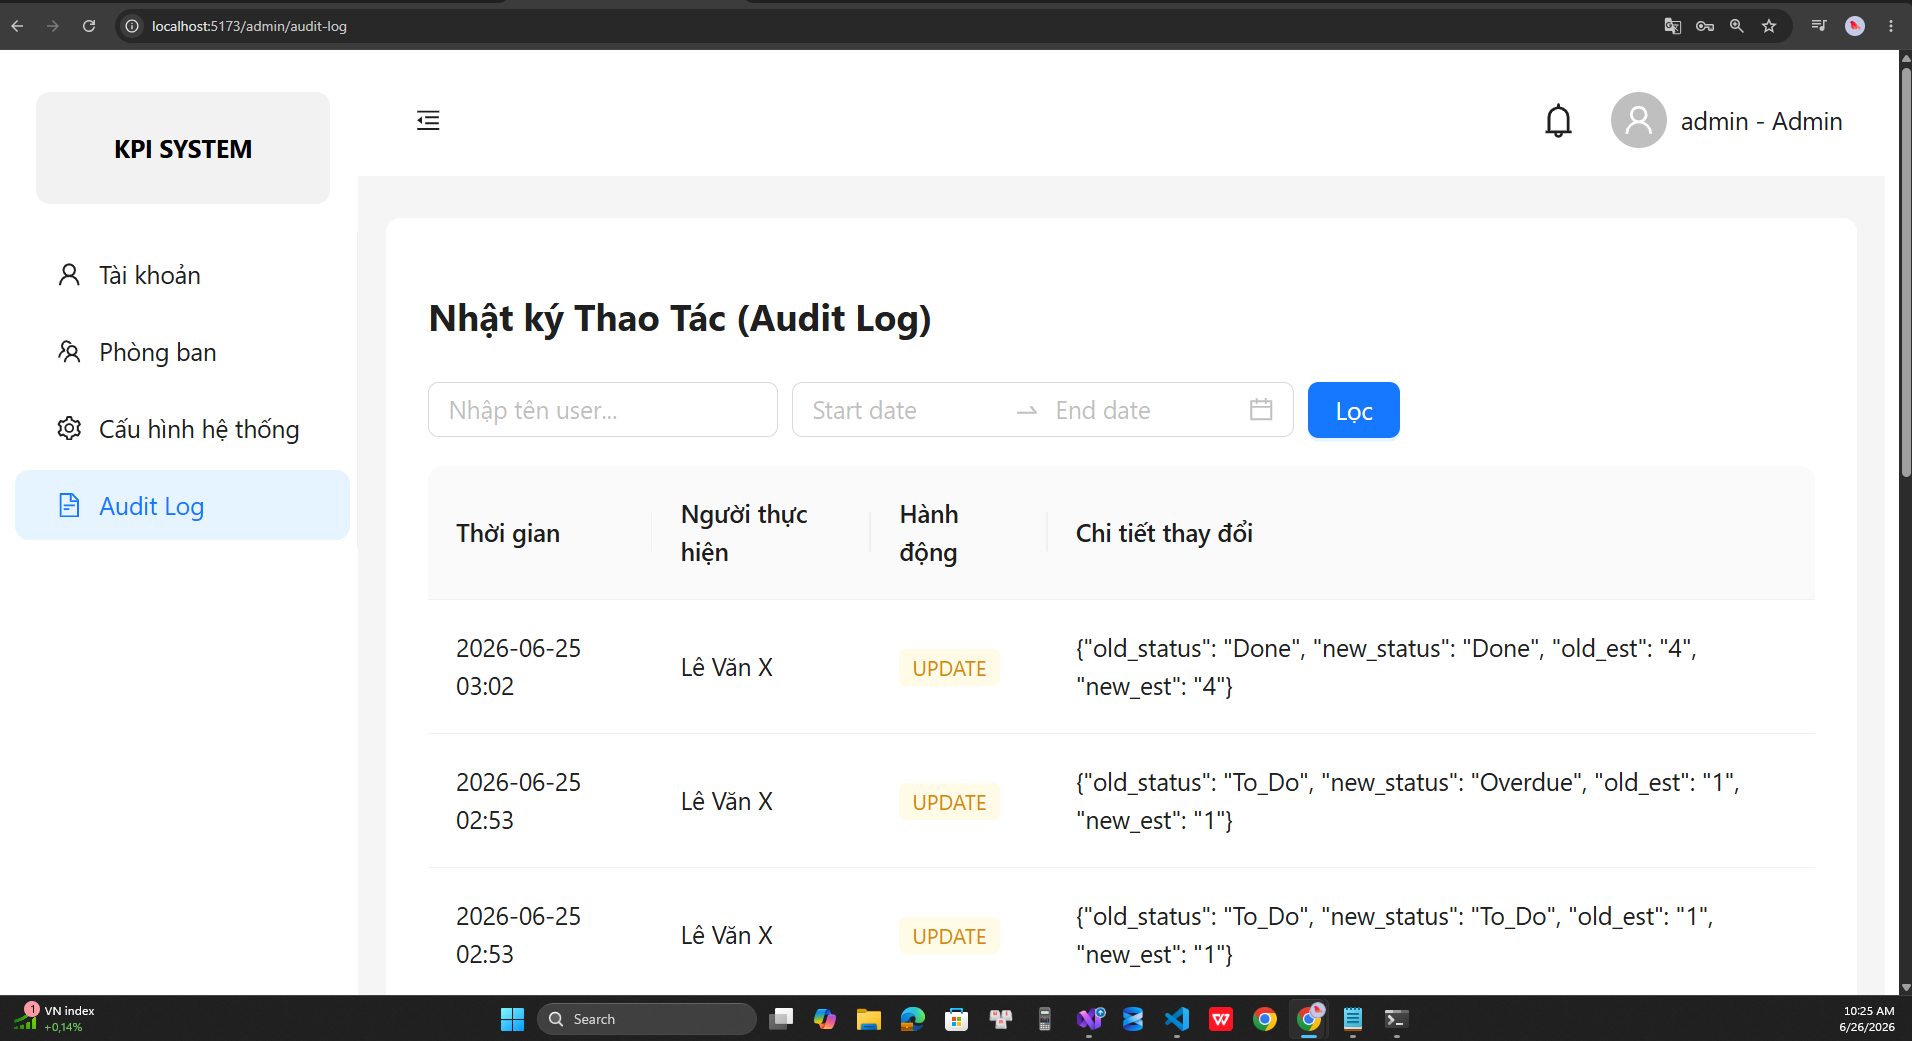
\includegraphics[width=0.95\textwidth]{audit_log_admin.png} % Đã khớp chính xác với tên file ảnh trong code của bạn
    \caption{Giao diện trang Nhật ký Thao tác (Audit Log) thực tế của hệ thống (Nguồn: Ảnh chụp màn hình ứng dụng)}
    \label{fig:demo_audit_log}
\end{figure}

\textbf{1. Giải thích chi tiết các thành phần dữ liệu và giao diện hiển thị}

Giao diện Nhật ký Thao tác được thiết kế theo cấu trúc bảng dữ liệu tối giản (\textit{Data Grid}), tập trung vào khả năng hiển thị thông tin rõ ràng và hỗ trợ truy vết lịch sử hệ thống theo thời gian thực. Dựa trên Hình \ref{fig:demo_audit_log}, giao diện bao gồm các cấu phần cốt lõi sau:
\begin{itemize}
    \item \textbf{Thanh điều hướng lề trái (Sidebar Navigation):} Chứa các menu chức năng quản trị hệ thống, bao gồm: "Tài khoản", "Phòng ban", "Cấu hình hệ thống", và mục "Audit Log" đang được kích hoạt làm nổi bật bằng nền xanh dương nhạt.
    \item \textbf{Bộ lọc tìm kiếm nâng cao (Filter Bar):} Nằm ngay phía trên bảng dữ liệu, cung cấp ô nhập liệu "Nhập tên nhân viên..." kết hợp với bộ chọn khung thời gian "Start date - End date". Đi kèm là nút lệnh "Lọc" màu xanh dương nổi bật, cho phép Admin nhanh chóng truy vấn các bản ghi theo điều kiện cụ thể mà không làm tải lại toàn bộ trang giấy nhờ kiến trúc SPA.
    \item \textbf{Bảng dữ liệu cấu trúc vết thao tác (Audit Log Table):} Bảng dữ liệu chính hiển thị tường minh luồng biến động thông tin với 4 cột dữ liệu cốt lõi:
    \begin{itemize}
        \item \textit{Thời gian:} Ghi nhận chính xác mốc thời gian phát sinh thao tác đến từng giây (\textit{Timestamp}) dựa trên múi giờ hệ thống máy chủ.
        \item \textit{Người thực hiện:} Định danh chính xác họ và tên của nhân sự thực hiện hành động làm thay đổi dữ liệu (Ví dụ: Lê Văn X, Vũ Văn X, Mã Gia L).
        \item \textit{Hành động:} Định nghĩa loại tác động nghiệp vụ (Ví dụ nhãn màu vàng chữ in hoa \texttt{UPDATE} cho các thao tác cập nhật dữ liệu).
        \item \textit{Chi tiết thay đổi:} Đây là phần cốt lõi của tính năng an toàn thông tin, hiển thị dữ liệu biến động dưới cấu trúc chuỗi \textit{JSON thô} trích xuất trực tiếp từ SQL Server (Ví dụ: \texttt{\{"old\_status":"To\_Do", "new\_status":"Done", "old\_est":"4", "new\_est":"4"\}}). Định dạng này giúp ghi vết tuyệt đối các giá trị cũ (\textit{Old value}) và giá trị mới (\textit{New value}) của thuộc tính trạng thái hoặc giờ nỗ lực.
    \end{itemize}
    \item \textbf{Thanh phân trang tự động (Pagination):} Nằm ở góc dưới cùng bên phải, cho phép giới hạn số lượng bản ghi hiển thị mặc định (Ví dụ: 10 dòng/trang) và hỗ trợ điều hướng nhanh qua các trang bằng các nút số tương tác, đảm bảo tốc độ phản hồi API luôn duy trì dưới mức $500ms$ bất kể độ phình to của cơ sở dữ liệu.
\end{itemize}

\textbf{2. Chi tiết các bước thao tác vận hành trên phần mềm (Demo User Flow)}

Để đảm bảo hệ thống vận hành trơn tru, Quản trị viên thực hiện các thao tác quản trị và giám sát hệ thống theo hai kịch bản nghiệp vụ chính dưới đây:

\textbf{Kịch bản A: Thiết lập cấu hình Kỳ đánh giá và Hệ số phạt}
\begin{itemize}
    \item \textbf{Bước 1: Khởi tạo kỳ đánh giá.} Admin tương tác với thanh menu bên lề trái, truy cập vào tab "Cấu hình Hệ thống" và nhấn nút "Tạo kỳ đánh giá mới". Hệ thống hiển thị một biểu mẫu nhập liệu dạng cửa sổ nổi (\textit{Modal Window}).
    \item \textbf{Bước 2: Nhập tham số vận hành.} Admin nhập tên kỳ (Ví dụ: \textit{KPI Tháng 10}). Sử dụng công cụ chọn ngày (\textit{Date Picker}) để xác định mốc thời gian từ $01/10$ đến $31/10$. Đặc biệt, Admin phải tính toán số ngày làm việc thực tế (trừ Thứ 7, Chủ Nhật và ngày Lễ) để nhập vào ô "Số giờ làm chuẩn trong tháng" (Ví dụ: 22 ngày $\times$ 8 giờ = 176 giờ). Thông số 176 giờ này sẽ là mẫu số đầu vào quan trọng để thuật toán hệ thống tính toán chỉ số Khối lượng ($P_3$) cho toàn bộ nhân sự kỹ thuật sau này.
    \item \textbf{Bước 3: Tùy chỉnh hệ số và Lưu dữ liệu.} Admin tinh chỉnh trường "Hệ số phạt trễ tiến độ" ở mức $0.9$ (giảm $10\%$ điểm số thành phần nếu vi phạm). Sau khi rà soát, Admin nhấn nút "Lưu cấu hình". Hệ thống \textit{Backend} tiếp nhận \textit{HTTP POST Request}, tiến hành kiểm tra tính hợp lệ dữ liệu và trả về thông báo trạng thái dạng \textit{Toast Notification} màu xanh góc phải màn hình báo hiệu cập nhật thành công.
\end{itemize}

\textbf{Kịch bản B: Tra cứu Nhật ký hệ thống (Audit Log) để kiểm tra luồng tiến độ công việc}
Giả sử cấp quản lý cần kiểm tra lịch sử kéo thả các thẻ công việc trên bảng Kanban của nhân sự kỹ thuật để rà soát tiến độ thực tế, Admin tiến hành truy vết trên giao diện thực nghiệm:
\begin{itemize}
    \item \textbf{Bước 1: Truy cập và Lọc dữ liệu.} Admin mở trang "Nhật ký Thao tác (Audit Log)" như minh họa tại Hình \ref{fig:demo_audit_log}. Tại thanh công cụ tìm kiếm phía trên, Admin nhập tên nhân viên cần kiểm tra vào ô trống (Ví dụ: "Lê Văn X"), sau đó nhấn nút lệnh "Lọc" màu xanh dương. Giao diện ngay lập tức cập nhật dữ liệu bảng và chỉ hiển thị các hành động liên quan đến nhân sự này.
    \item \textbf{Bước 2: Phân tích bản ghi thao tác.} Hệ thống trả về danh sách các thao tác đã bị lọc theo dòng. Admin tiến hành quan sát cột "Hành động" để tìm kiếm các nhãn màu vàng mang giá trị \texttt{UPDATE} – đại diện cho các hành động thay đổi trạng thái thẻ công việc hoặc chỉnh sửa thông tin.
    \item \textbf{Bước 3: Đối chiếu chuỗi dữ liệu JSON.} Tại cột "Chi tiết thay đổi", Admin đọc trực tiếp cấu trúc dữ liệu lưu vết dạng cặp khóa - giá trị của đối tượng JSON. Bản ghi hiển thị rành rọt: thuộc tính trạng thái công việc đã có sự dịch chuyển từ giá trị cũ \texttt{"old\_status":"To\_Do"} sang giá trị mới \texttt{"new\_status":"Overdue"} hoặc \texttt{"new\_status":"Done"}. Sự minh bạch của nguồn dữ liệu thô không thể chối cãi này giúp Ban Giám đốc nắm bắt chính xác tiến trình xử lý công việc thực tế của kỹ sư mà không cần thông qua các báo cáo thủ công.
\end{itemize}

\subsection{Phân hệ Quản lý Dự án (Sơ đồ Gantt, Giao việc, Duyệt Log-time)}

Phân hệ Quản lý Dự án (Project Management Module) đóng vai trò là "không gian chỉ huy chiến thuật" dành riêng cho Quản lý dự án (Project Manager - PM). Tại đây, mọi tư duy hoạch định vĩ mô được hiện thực hóa thành các khối công việc vi mô, đồng thời là nơi PM thực thi quyền lực giám sát và đánh giá chất lượng nguồn lực. Giao diện của phân hệ này được thiết kế tập trung vào việc tối ưu hóa khả năng quan sát (Observability) và giảm thiểu số lượng thao tác chuột (Click-through Rate) cho các tác vụ quản trị hàng ngày.

% --- ẢNH 1: SƠ ĐỒ GANTT ---
\begin{figure}[H]
    \centering
    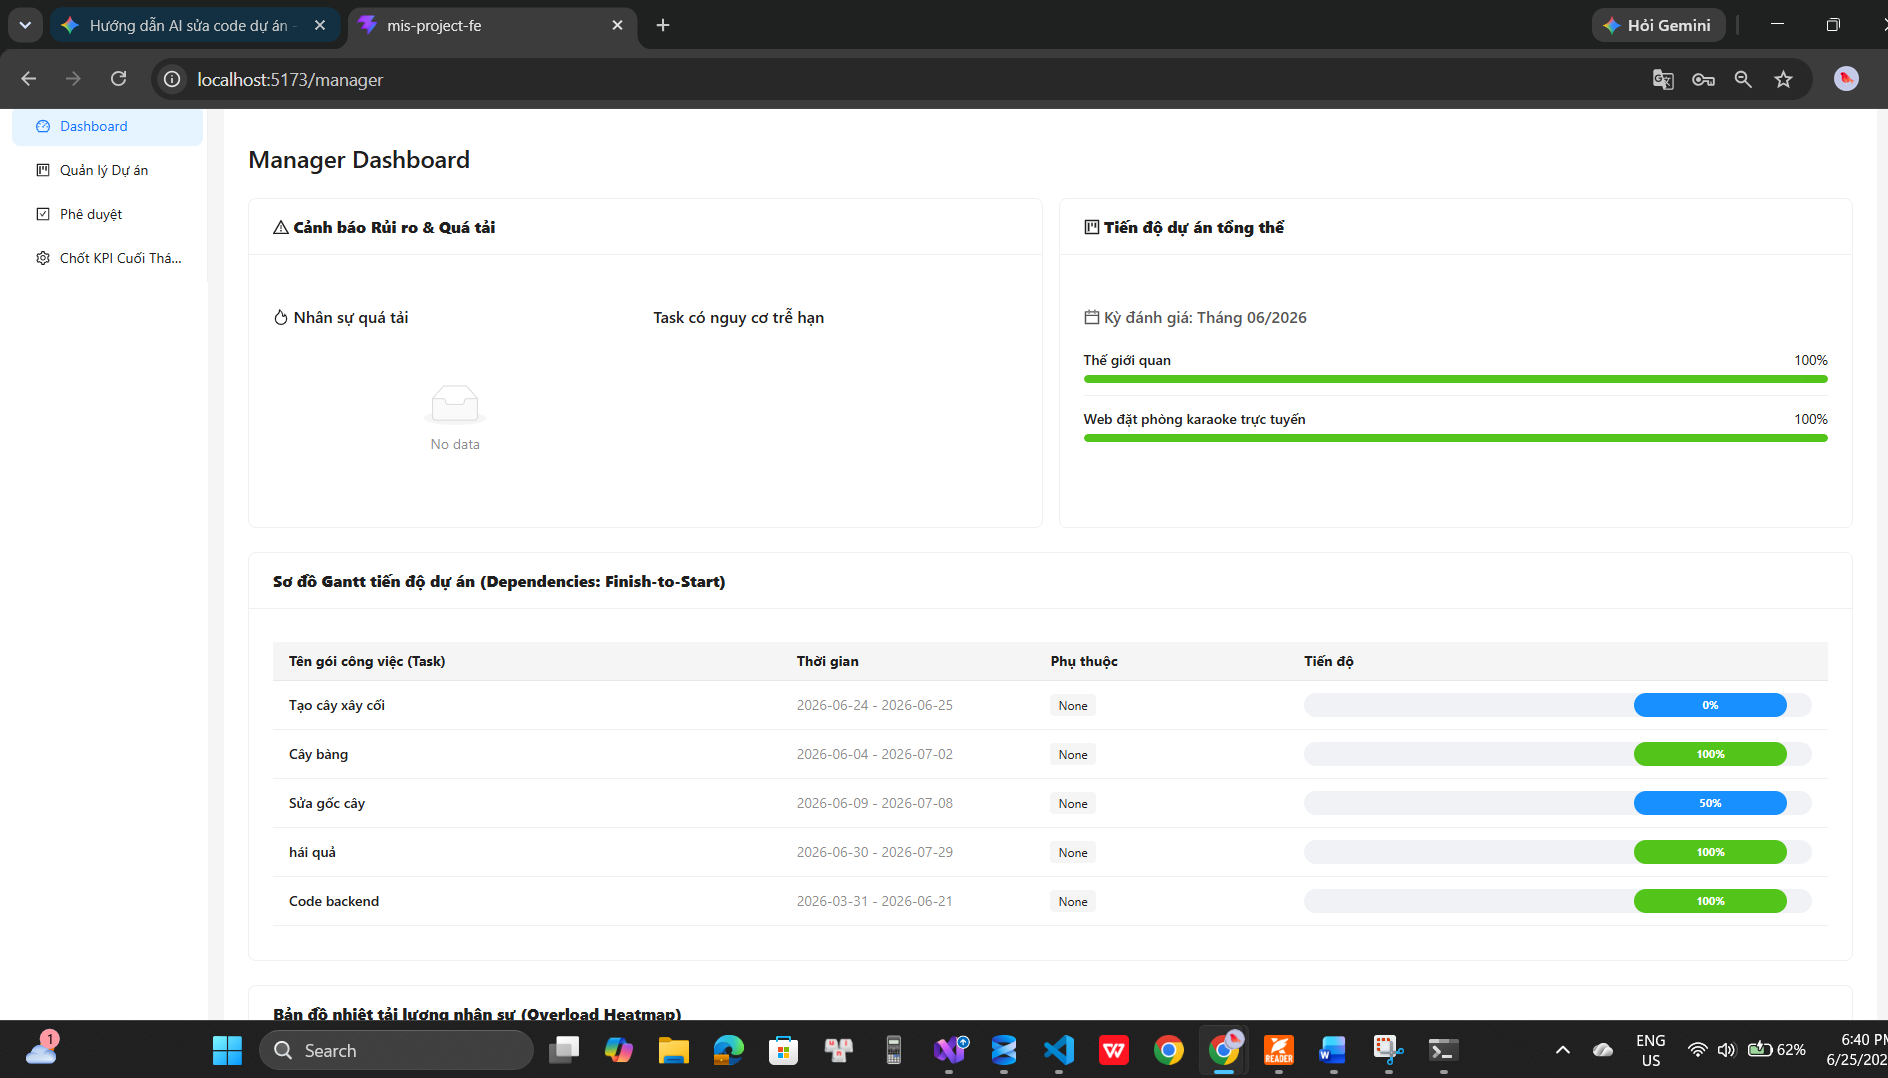
\includegraphics[width=0.85\textwidth]{gantt.png} % Tên file ảnh sơ đồ Gantt
    \caption{Phân hệ Quản lý dự án - Sơ đồ Gantt (Nguồn: Tác giả tự chụp màn hình)}
    \label{fig:gantt}
\end{figure}

% --- ẢNH 2: DANH SÁCH PHÊ DUYỆT ---
\begin{figure}[H]
    \centering
    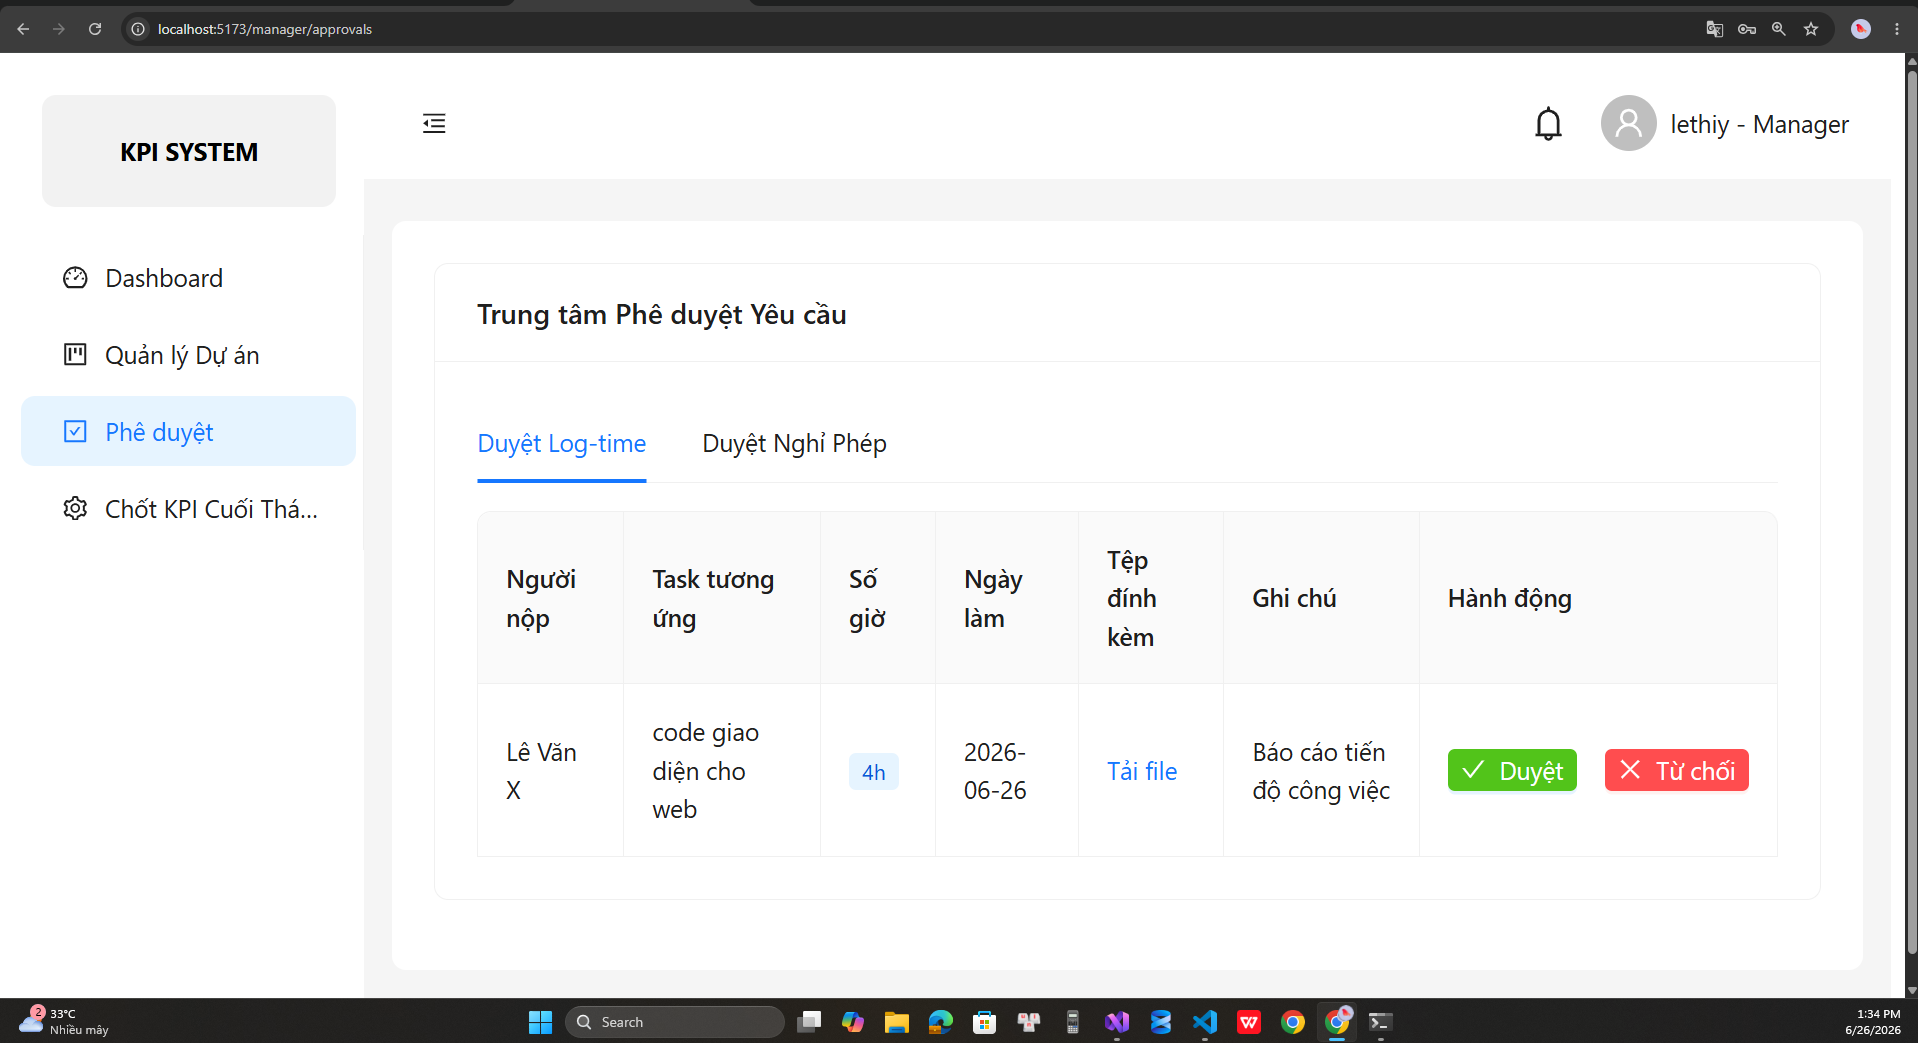
\includegraphics[width=0.85\textwidth]{man_hinh_phe_duyet.png} % Tên file ảnh danh sách phê duyệt
    \caption{Phân hệ Quản lý dự án - Danh sách phê duyệt (Nguồn: Tác giả tự chụp màn hình)}
    \label{fig:approval}
\end{figure}

% --- ẢNH 3: GIAO VIỆC (MỚI THÊM) ---
\begin{figure}[H]
    \centering
    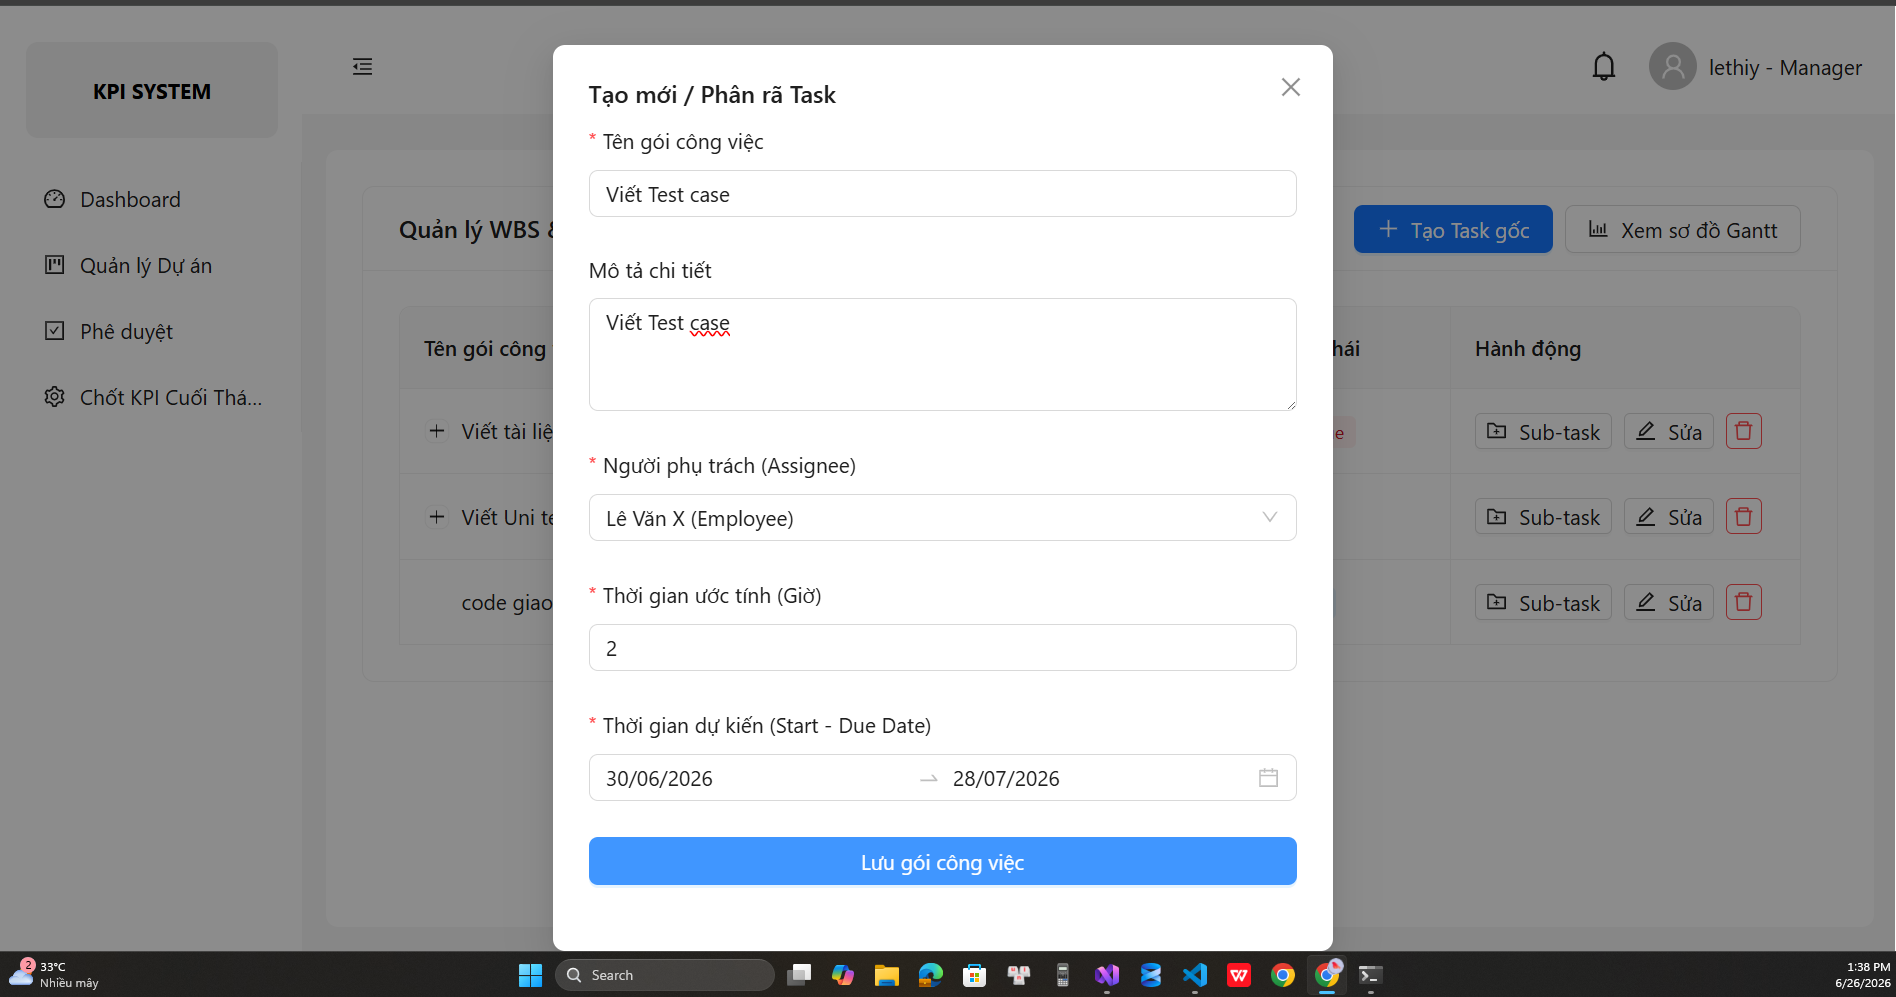
\includegraphics[width=0.85\textwidth]{mh_giao_viec.png} % Thay bằng tên file ảnh giao việc của bạn
    \caption{Phân hệ Quản lý dự án - Giao việc (Nguồn: Tác giả tự chụp màn hình)}
    \label{fig:assignment}
\end{figure}



\textbf{1. Giải thích chi tiết giao diện trực quan và cơ chế hiển thị của Nhân sự}

Giao diện không gian làm việc của Employee được thiết kế tối giản, phân bố qua thanh điều hướng bên trái (Sidebar) với các phân hệ chính: \textit{Trang chủ, Công việc, Lịch sử Log-time, và Xin nghỉ phép}. 

\begin{itemize}
    \item \textbf{Tổng quan (Employee Dashboard - Trang chủ):} Đây là màn hình đầu tiên nhân sự nhìn thấy khi đăng nhập, đóng vai trò như một bộ tản nhiệt thông tin cá nhân. Khu vực "Theo dõi KPI cá nhân (Tháng này)" trực quan hóa thuật toán KPI thành 4 thanh tiến trình (Progress Bars) tương ứng với 4 trọng số: \textit{Tiến độ (40\%), Hiệu suất (30\%), Khối lượng (20\%), và Điểm Quản lý (10\%)}. Các thanh tiến trình này (như hình minh họa hiển thị Tiến độ đạt $95.29\%$) được cập nhật dữ liệu theo thời gian thực, giúp nhân sự tự đánh giá năng suất. Kế bên là khu vực "Công việc sắp đến hạn (Due Soon)", liệt kê các tác vụ cấp bách kèm nhãn trạng thái (\textit{Cần làm, Đang làm}) để định hướng ưu tiên công việc trong ngày.
    
    \item \textbf{Bảng Công việc (Kanban Board):} Khi truy cập tab "Công việc", hệ thống cung cấp một hộp thoại thả xuống (Dropdown) để nhân sự lọc \textit{Task} theo từng dự án cụ thể (Ví dụ: Dự án "Thế giới quan"). Bảng Kanban được chuẩn hóa với ba cột trạng thái cốt lõi: \textit{To-Do (Cần làm), Doing (Đang làm), và Done (Đã xong)}.
    
    \item \textbf{Cấu trúc Thẻ công việc (Task Card):} Tại cột \textit{Done}, mỗi thẻ tác vụ (Ví dụ: "Cây bàng" hoặc "Code backend") được đóng gói gọn gàng. Thẻ hiển thị trực tiếp Tên công việc, icon đồng hồ kèm Số giờ dự kiến (\textit{Est: 4h}), và một nhãn (Tag) màu xanh định danh người phụ trách (\textit{Assignee}), đảm bảo thông tin minh bạch và dễ quét bằng mắt.
\end{itemize}

\textbf{2. Mô tả chi tiết luồng thao tác cập nhật tiến độ và Log-time (Demo User Flow)}

Để cập nhật tiến độ và nộp dữ liệu chấm công, nhân sự thực hiện chuỗi thao tác được kiểm soát bằng các ràng buộc nhập liệu (Form Validation) chặt chẽ trên hệ thống như sau:

\begin{itemize}
    \item \textbf{Bước 1: Điều hướng và Tương tác Kanban.} Tại màn hình Bảng Công việc, nhân viên chọn dự án tương ứng. Quá trình làm việc được ghi nhận thông qua thao tác kéo-thả thẻ (Drag \& Drop) từ cột \textit{To-Do} sang \textit{Doing}.
    
    \item \textbf{Bước 2: Hoàn thành và Mở chi tiết Task.} Khi công việc hoàn tất, nhân viên kéo thẻ sang cột \textit{Done} hoặc click trực tiếp vào thẻ. Hệ thống lập tức hiển thị một Cửa sổ nổi (\textit{Modal Window}) mang tên "Chi tiết: [Tên công việc]".
    
    \item \textbf{Bước 3: Xử lý các hành động phụ trợ (Optional).} Tại Modal chi tiết, trước khi điền form, hệ thống cung cấp các nút hành động phụ. Nếu công việc gặp trục trặc không thể hoàn thành, nhân viên có thể nhấn nút "Xin gia hạn thời gian". Nếu kéo nhầm, có thể chọn "Hủy nộp Log-time".
    
    \item \textbf{Bước 4: Khai báo Form nộp báo cáo thời gian thực tế.} Đây là bước bắt buộc. Nhân sự phải điền dữ liệu vào các trường thông tin:
        \begin{itemize}
            \item \textit{Trường bắt buộc (Đánh dấu * đỏ):} Nhập số liệu vào ô "Số giờ làm việc thực tế (Giờ)" (Ví dụ: 4.5) và sử dụng \textit{Date Picker} để chọn "Ngày thực hiện". Hệ thống sẽ báo lỗi nếu bỏ trống hai trường này.
            \item \textit{Trường tùy chọn:} Khai báo thêm chi tiết vào ô "Ghi chú" (Tóm tắt công việc đã làm) và sử dụng nút "Chọn file" tại mục "Đính kèm file bằng chứng" để upload tài liệu/hình ảnh chứng minh kết quả.
        \end{itemize}
    
    \item \textbf{Bước 5: Đệ trình và Thảo luận.} Sau khi rà soát, nhân viên nhấn nút \textbf{"Gửi yêu cầu duyệt Log-time"} màu xanh lam để hoàn tất. Dữ liệu sẽ được khóa lại và đẩy sang phân hệ phê duyệt của Manager. Ngoài ra, ở góc dưới của Modal còn tích hợp tính năng "Thảo luận / Bình luận", cho phép nhân viên và quản lý trao đổi trực tiếp các vấn đề phát sinh ngay trên từng Task cụ thể mà không cần sử dụng ứng dụng chat bên ngoài.
\end{itemize}
\subsection{Phân hệ Nhân sự (Bảng Kanban, Báo cáo tiến độ cá nhân)}

Nếu Phân hệ Quản trị là "buồng lái" của cấp quản lý, thì Phân hệ Nhân sự (Employee Dashboard) chính là "tiền tuyến" (Frontline) của hệ thống MIS. Đây là không gian làm việc số hàng ngày của lực lượng thực thi (Developer, Tester, BA), nơi trực tiếp sinh ra các nguồn dữ liệu sơ cấp (Primary Data) như trạng thái công việc và số giờ làm thực tế. Thiết kế của phân hệ này đặt sự tối giản và tính khả dụng (Usability) lên hàng đầu, nhằm triệt tiêu tối đa "độ ma sát" (Friction) trong quá trình nhân viên cập nhật thông tin, đảm bảo họ không cảm thấy bị biến thành những "cỗ máy nhập liệu".

% --- ẢNH 4: GIAO DIỆN BẢNG KANBAN ---
\begin{figure}[H] % [H] giữ ảnh cố định tại đây như Word
    \centering
    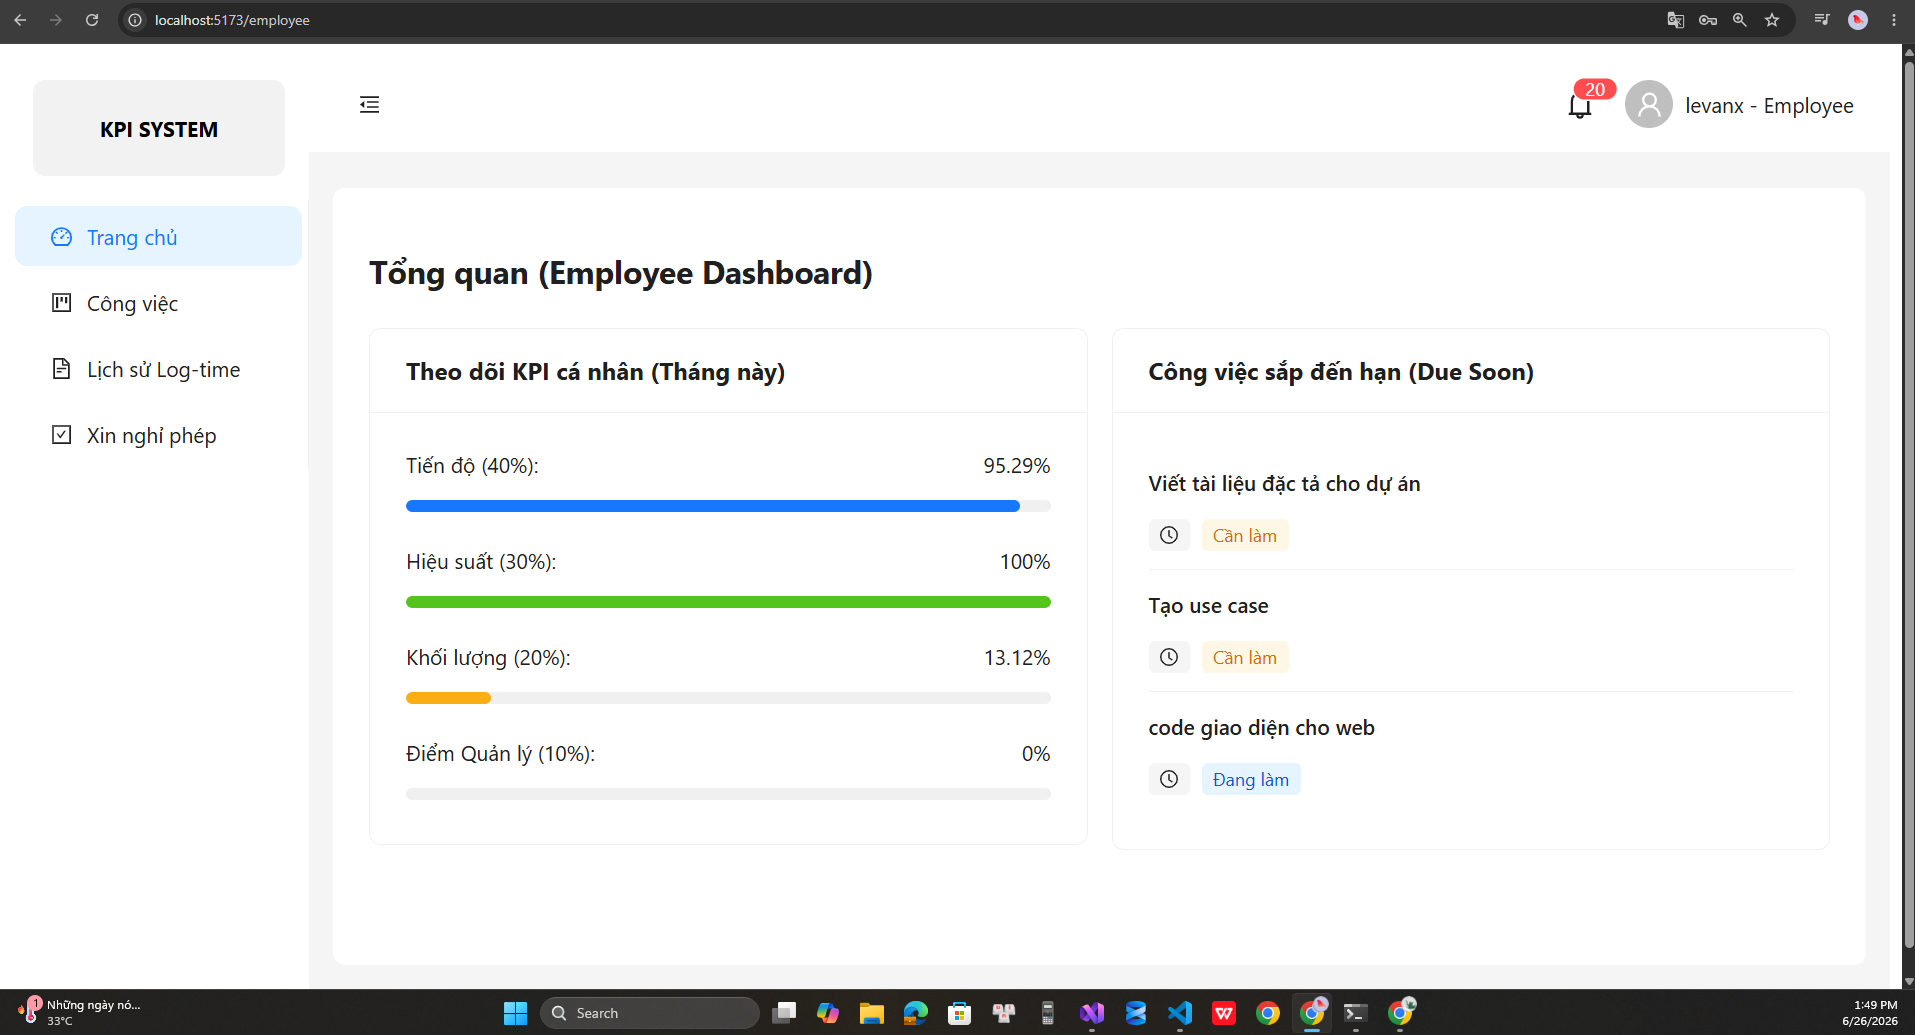
\includegraphics[width=0.85\textwidth]{kaban_personal.png} % Thay bằng tên file ảnh bảng Kanban của bạn
    \caption{Phân hệ nhân sự - Giao diện bảng Kanban (Nguồn: Tác giả tự chụp màn hình)}
    \label{fig:kanban}
\end{figure}

% --- ẢNH 5: FORM BÁO CÁO TIẾN ĐỘ ---
\begin{figure}[H] 
    \centering
    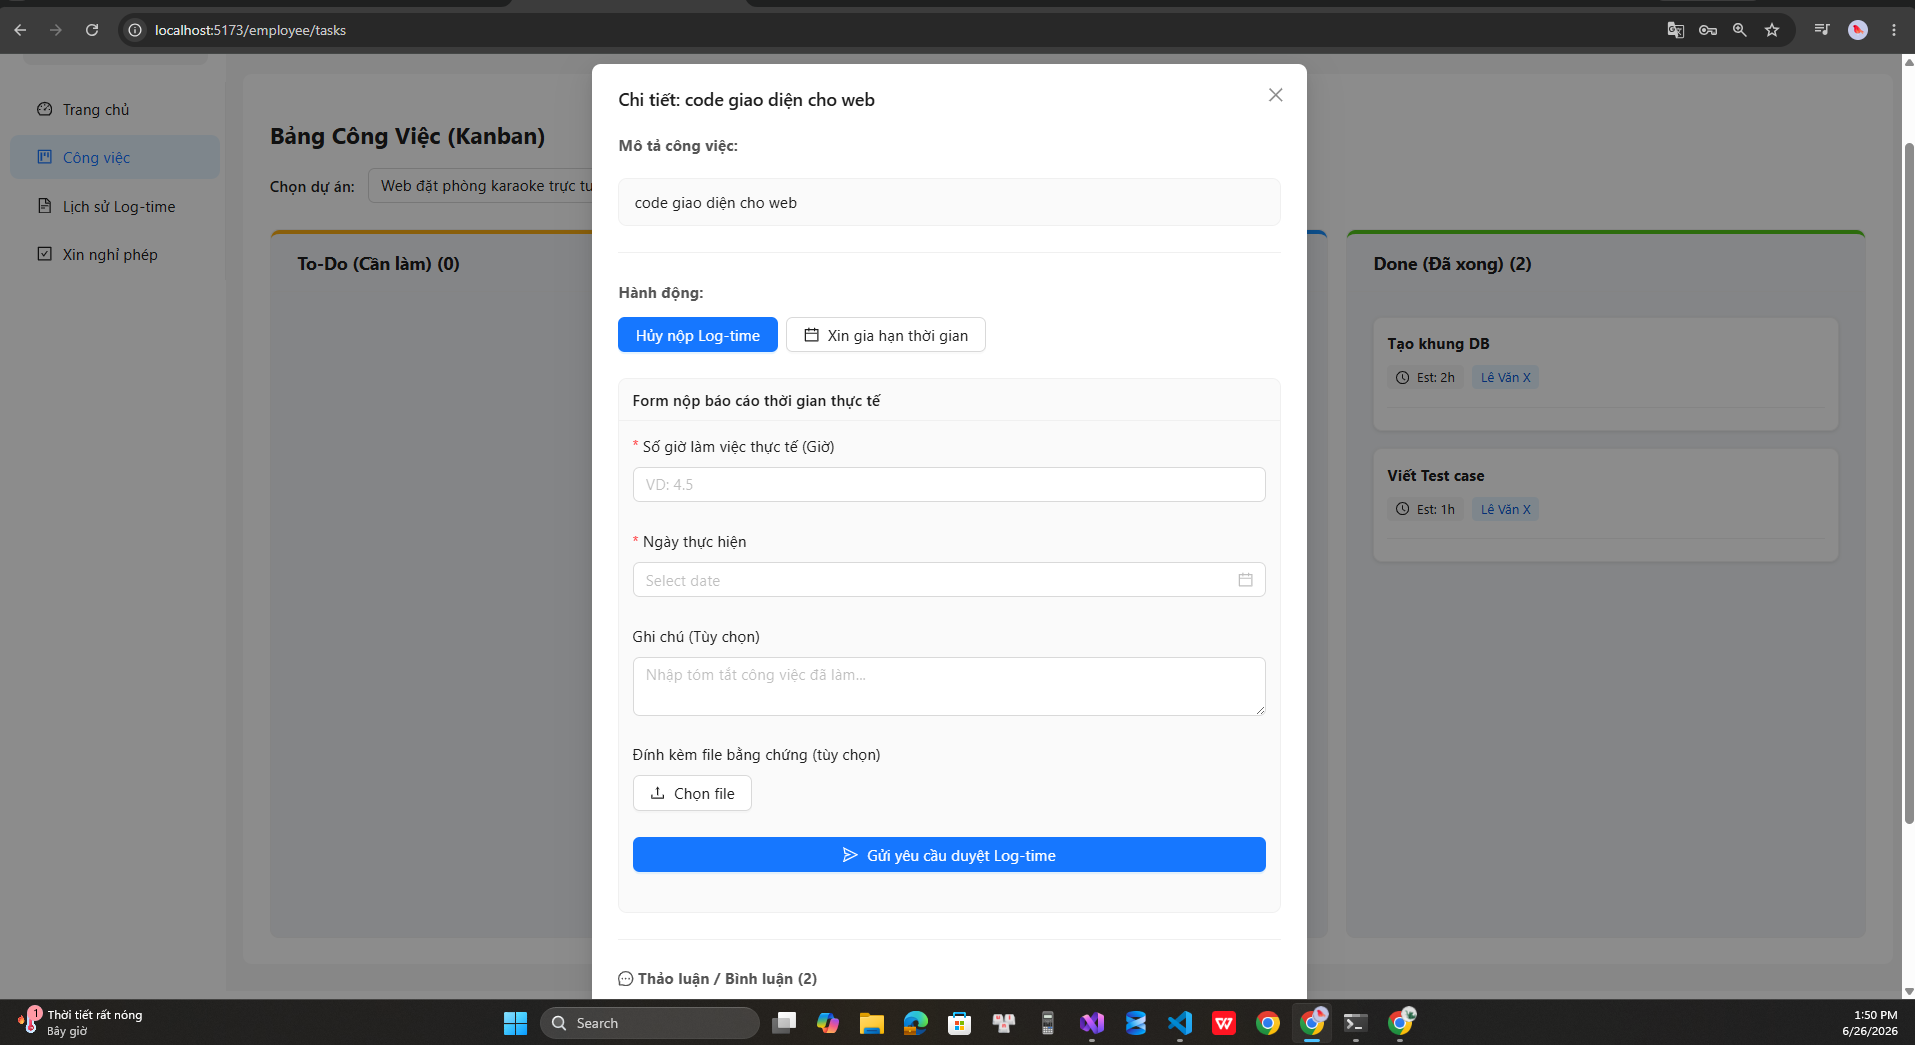
\includegraphics[width=0.85\textwidth]{mh_bcao_tien_do.png} % Thay bằng tên file ảnh Form báo cáo của bạn
    \caption{Phân hệ nhân sự - Form báo cáo tiến độ (Nguồn: Tác giả tự chụp màn hình)}
    \label{fig:progress_report}
\end{figure}


\textbf{1. Giải thích chi tiết giao diện trực quan và cơ chế hiển thị của Nhân sự}

Giao diện không gian làm việc của Employee được thiết kế tối giản, phân bố qua thanh điều hướng bên trái (Sidebar) với các phân hệ chính: \textit{Trang chủ, Công việc, Lịch sử Log-time, và Xin nghỉ phép}. 

\begin{itemize}
    \item \textbf{Tổng quan (Employee Dashboard - Trang chủ):} Đây là màn hình đầu tiên nhân sự nhìn thấy khi đăng nhập, đóng vai trò như một bộ tản nhiệt thông tin cá nhân. Khu vực "Theo dõi KPI cá nhân (Tháng này)" trực quan hóa thuật toán KPI thành 4 thanh tiến trình (Progress Bars) tương ứng với 4 trọng số: \textit{Tiến độ (40\%), Hiệu suất (30\%), Khối lượng (20\%), và Điểm Quản lý (10\%)}. Các thanh tiến trình này (như hình minh họa hiển thị Tiến độ đạt $95.29\%$) được cập nhật dữ liệu theo thời gian thực, giúp nhân sự tự đánh giá năng suất. Kế bên là khu vực "Công việc sắp đến hạn (Due Soon)", liệt kê các tác vụ cấp bách kèm nhãn trạng thái (\textit{Cần làm, Đang làm}) để định hướng ưu tiên công việc trong ngày.
    
    \item \textbf{Bảng Công việc (Kanban Board):} Khi truy cập tab "Công việc", hệ thống cung cấp một hộp thoại thả xuống (Dropdown) để nhân sự lọc \textit{Task} theo từng dự án cụ thể (Ví dụ: Dự án "Thế giới quan"). Bảng Kanban được chuẩn hóa với ba cột trạng thái cốt lõi: \textit{To-Do (Cần làm), Doing (Đang làm), và Done (Đã xong)}.
    
    \item \textbf{Cấu trúc Thẻ công việc (Task Card):} Tại cột \textit{Done}, mỗi thẻ tác vụ (Ví dụ: "Cây bàng" hoặc "Code backend") được đóng gói gọn gàng. Thẻ hiển thị trực tiếp Tên công việc, icon đồng hồ kèm Số giờ dự kiến (\textit{Est: 4h}), và một nhãn (Tag) màu xanh định danh người phụ trách (\textit{Assignee}), đảm bảo thông tin minh bạch và dễ quét bằng mắt.
\end{itemize}

\textbf{2. Mô tả chi tiết luồng thao tác cập nhật tiến độ và Log-time (Demo User Flow)}

Để cập nhật tiến độ và nộp dữ liệu chấm công, nhân sự thực hiện chuỗi thao tác được kiểm soát bằng các ràng buộc nhập liệu (Form Validation) chặt chẽ trên hệ thống như sau:

\begin{itemize}
    \item \textbf{Bước 1: Điều hướng và Tương tác Kanban.} Tại màn hình Bảng Công việc, nhân viên chọn dự án tương ứng. Quá trình làm việc được ghi nhận thông qua thao tác kéo-thả thẻ (Drag \& Drop) từ cột \textit{To-Do} sang \textit{Doing}.
    
    \item \textbf{Bước 2: Hoàn thành và Mở chi tiết Task.} Khi công việc hoàn tất, nhân viên kéo thẻ sang cột \textit{Done} hoặc click trực tiếp vào thẻ. Hệ thống lập tức hiển thị một Cửa sổ nổi (\textit{Modal Window}) mang tên "Chi tiết: [Tên công việc]".
    
    \item \textbf{Bước 3: Xử lý các hành động phụ trợ (Optional).} Tại Modal chi tiết, trước khi điền form, hệ thống cung cấp các nút hành động phụ. Nếu công việc gặp trục trặc không thể hoàn thành, nhân viên có thể nhấn nút "Xin gia hạn thời gian". Nếu kéo nhầm, có thể chọn "Hủy nộp Log-time".
    
    \item \textbf{Bước 4: Khai báo Form nộp báo cáo thời gian thực tế.} Đây là bước bắt buộc. Nhân sự phải điền dữ liệu vào các trường thông tin:
        \begin{itemize}
            \item \textit{Trường bắt buộc (Đánh dấu * đỏ):} Nhập số liệu vào ô "Số giờ làm việc thực tế (Giờ)" (Ví dụ: 4.5) và sử dụng \textit{Date Picker} để chọn "Ngày thực hiện". Hệ thống sẽ báo lỗi nếu bỏ trống hai trường này.
            \item \textit{Trường tùy chọn:} Khai báo thêm chi tiết vào ô "Ghi chú" (Tóm tắt công việc đã làm) và sử dụng nút "Chọn file" tại mục "Đính kèm file bằng chứng" để upload tài liệu/hình ảnh chứng minh kết quả.
        \end{itemize}
    
    \item \textbf{Bước 5: Đệ trình và Thảo luận.} Sau khi rà soát, nhân viên nhấn nút \textbf{"Gửi yêu cầu duyệt Log-time"} màu xanh lam để hoàn tất. Dữ liệu sẽ được khóa lại và đẩy sang phân hệ phê duyệt của Manager. Ngoài ra, ở góc dưới của Modal còn tích hợp tính năng "Thảo luận / Bình luận", cho phép nhân viên và quản lý trao đổi trực tiếp các vấn đề phát sinh ngay trên từng Task cụ thể mà không cần sử dụng ứng dụng chat bên ngoài.
\end{itemize}
\subsection{Phân hệ Báo cáo MIS (Dashboard tổng quan, Chốt KPI cuối tháng)}

Phân hệ Báo cáo MIS là tầng cao nhất trong kiến trúc hệ thống, đóng vai trò chuyển hóa những luồng dữ liệu thô (như số giờ Log-time, trạng thái Task) thành các tri thức quản trị chiến lược. Đây là không gian làm việc định hướng dữ liệu (Data-driven) dành riêng cho Ban Giám đốc (C-Level) để theo dõi sức khỏe toàn doanh nghiệp, và dành cho Quản lý (Manager) / Khối Nhân sự (HR) để thực thi công tác đánh giá, chốt sổ cuối kỳ.

% --- Lệnh chèn ảnh tự động bám sát ảnh thật ---
\begin{figure}[H]
    \centering
    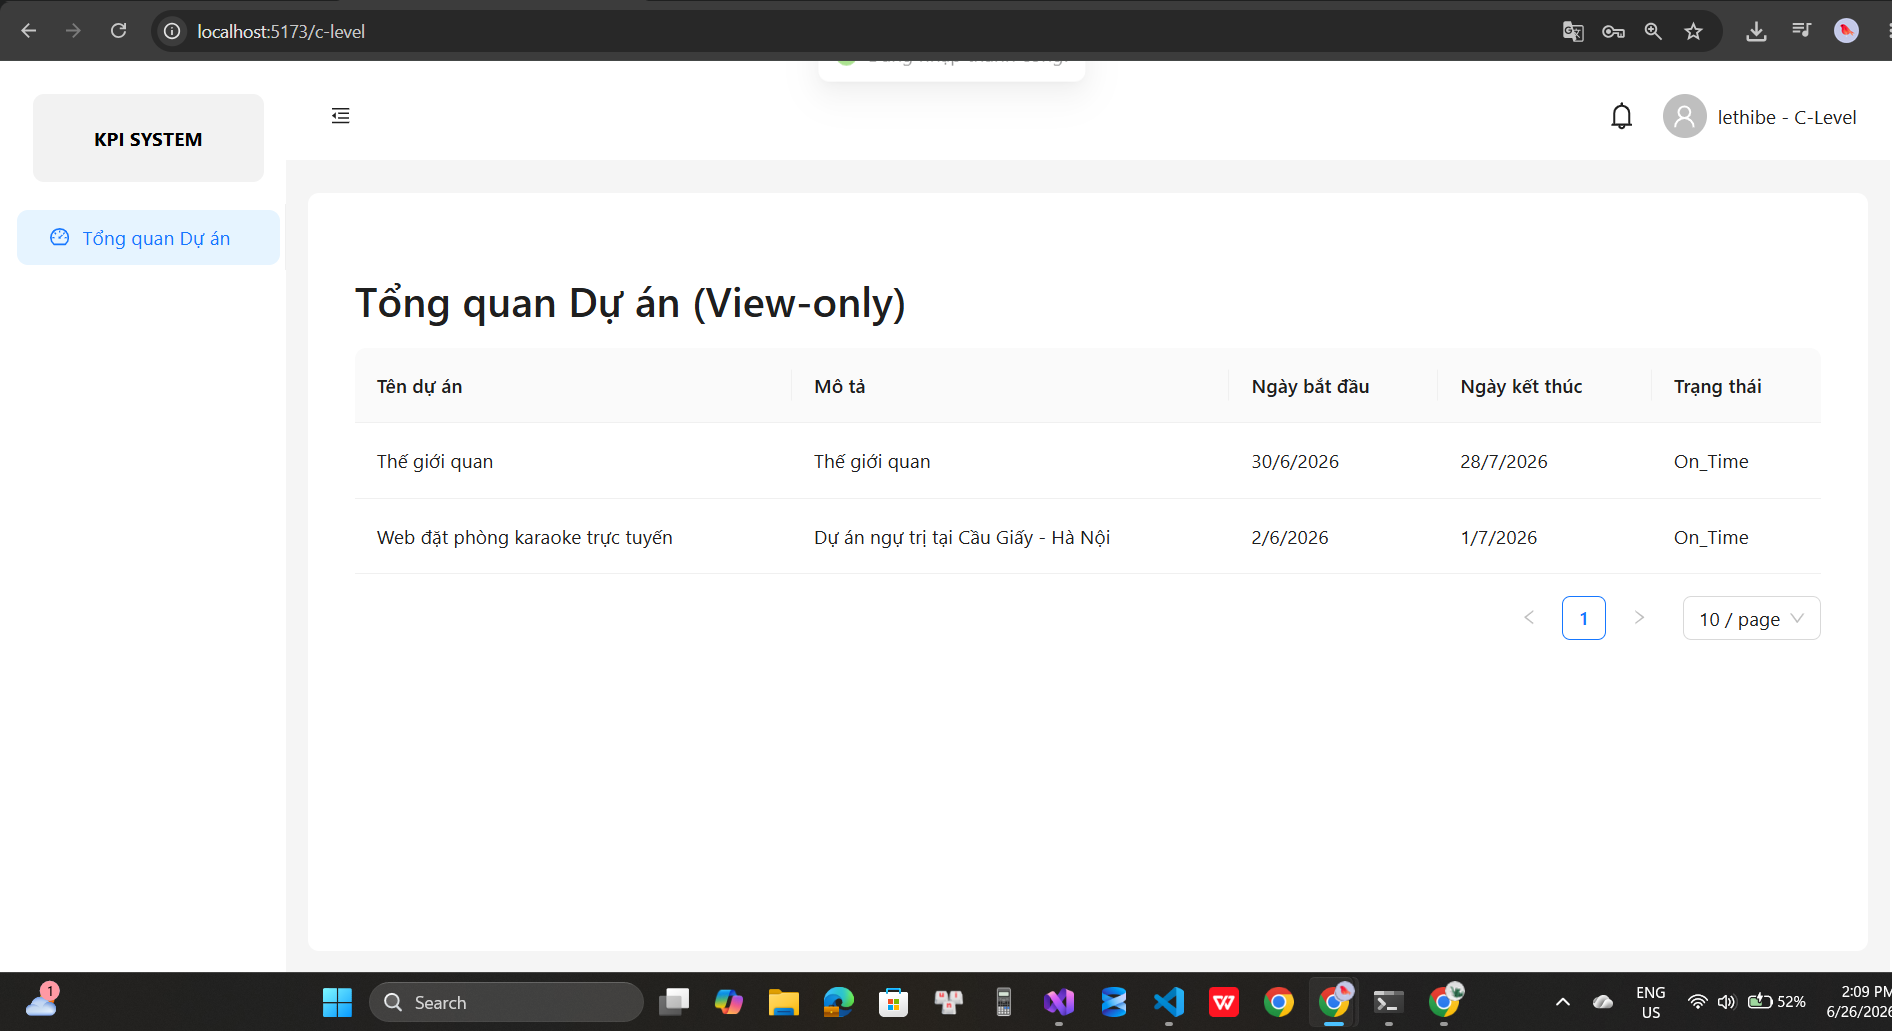
\includegraphics[width=1\textwidth]{c_level_view.png}
    \caption{Giao diện Tổng quan Dự án (View-only) dành cho Ban Giám đốc (C-Level) (Nguồn: Tác giả tự chụp màn hình)}
    \label{fig:clevel_dashboard}
\end{figure}

\begin{figure}[H]
    \centering
    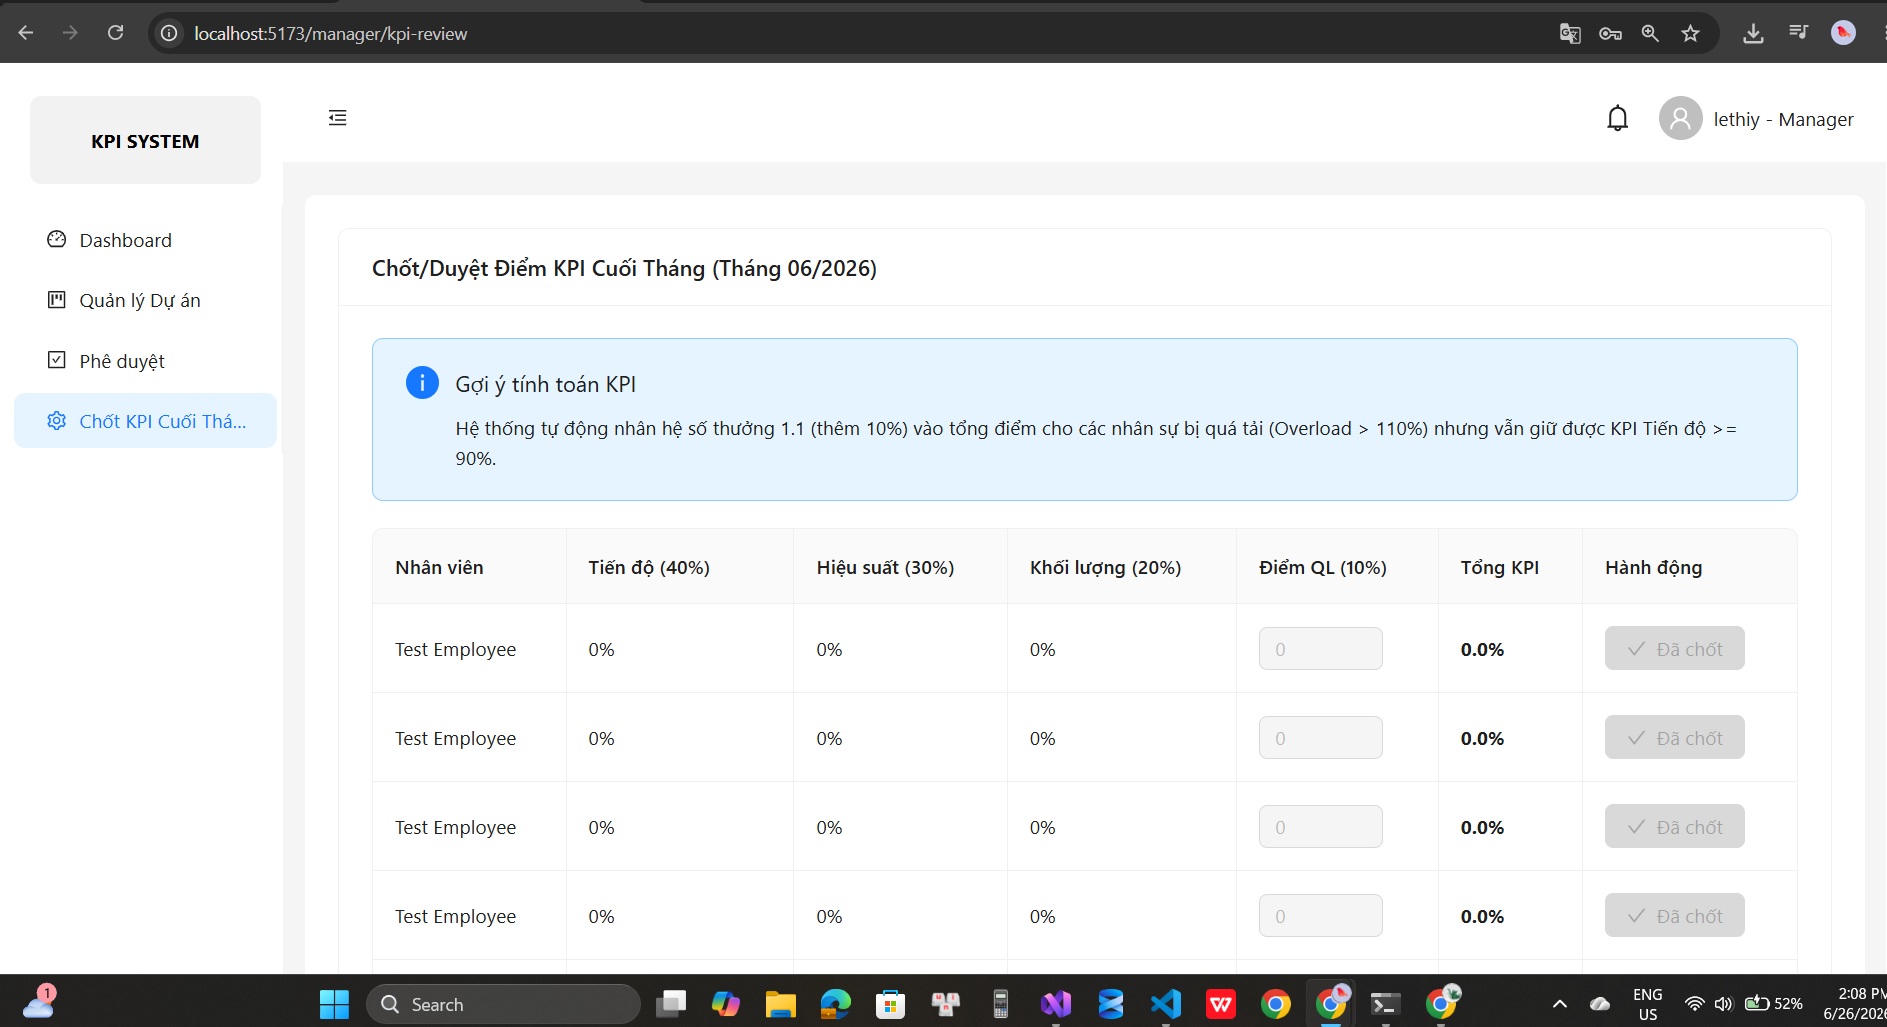
\includegraphics[width=1\textwidth]{chot_kpi.png}
    \caption{Giao diện Chốt/Duyệt Điểm KPI Cuối tháng dành cho Manager (Nguồn: Tác giả tự chụp màn hình)}
    \label{fig:kpi_review_dashboard}
\end{figure}

\textbf{1. Giải thích ý nghĩa của các Bảng điều khiển và Thống kê trực quan}

Hệ thống cung cấp các góc nhìn (Views) được thiết kế chuyên biệt, phân cấp theo đúng nguyên lý "đặc quyền thông tin":

\begin{itemize}
    \item \textbf{Góc nhìn của Ban Giám đốc (C-Level Dashboard):} Giao diện được thiết kế theo cơ chế \textit{View-only} (Chỉ xem) nhằm tránh các can thiệp thao tác nhầm lẫn. Bảng "Tổng quan Dự án" lược bỏ hoàn toàn các chi tiết vi mô (như thẻ Kanban hay Log-time cá nhân), thay vào đó tập trung hiển thị bức tranh vĩ mô. Ban Giám đốc có thể bao quát toàn bộ danh mục dự án đang chạy (Ví dụ: Dự án \textit{"Thế giới quan"}, \textit{"Web đặt phòng karaoke trực tuyến"}), đi kèm mốc thời gian (Ngày bắt đầu/kết thúc) và cột \textit{Trạng thái (Status)}. Nhờ các trạng thái được cập nhật \textit{Real-time} như \texttt{On\_Time} (Đúng tiến độ) hoặc \texttt{Overdue} (Trễ hạn), C-Level có thể ngay lập tức phát hiện dự án nào đang "cháy" để đưa ra chỉ đạo chiến lược.
    
    \item \textbf{Góc nhìn của Quản lý dự án (Manager Dashboard):} Tích hợp các bộ báo cáo cảnh báo sớm. Khu vực \textit{"Cảnh báo Rủi ro \& Quá tải"} đóng vai trò như một hệ thống radar, tự động rà quét và hiển thị danh sách các "Nhân sự quá tải" hoặc "Task có nguy cơ trễ hạn". Kế đó, biểu đồ thanh ngang \textit{"Tiến độ dự án tổng thể"} trực quan hóa tỷ lệ hoàn thành (Ví dụ: đạt $100\%$) của từng dự án trong kỳ đánh giá, giúp Manager phân bổ lại nguồn lực kịp thời.
    
    \item \textbf{Giao diện Chốt Điểm KPI (Bảng KPI Review):} Đây là kết quả đầu ra của Động cơ KPI Engine. Bảng dữ liệu hiển thị rành mạch 4 trụ cột đánh giá: \textit{Tiến độ (40\%), Hiệu suất (30\%), Khối lượng (20\%), và Điểm QL (10\%)}. Đặc biệt, hệ thống hiển thị một hộp thông báo \textit{Gợi ý tính toán KPI} màu xanh nổi bật, nhắc nhở Manager về cơ chế xử lý ngoại lệ: \textit{"Hệ thống tự động nhân hệ số thưởng 1.1 (thêm 10\%) vào tổng điểm cho các nhân sự bị quá tải (Overload > 110\%) nhưng vẫn giữ được KPI Tiến độ $\ge$ 90\%"}.
\end{itemize}

\textbf{2. Luồng thao tác khóa cổng nhập liệu và Chốt sổ KPI cuối kỳ}

Để đảm bảo dữ liệu tính lương (Payroll) không bị sai lệch, công tác chốt sổ KPI vào ngày cuối tháng được hệ thống kiểm soát qua một luồng quy trình khép kín:

\begin{itemize}
    \item \textbf{Bước 1: Đóng băng dữ liệu (Data Freezing).} Vào lúc 23:59 ngày cuối cùng của kỳ đánh giá, \textit{Background Job (Hangfire)} sẽ tự động kích hoạt. Hệ thống khóa toàn bộ các \textit{Form Log-time} của kỳ hiện tại; nhân sự không thể thêm mới hay chỉnh sửa giờ làm. Ngay sau đó, thuật toán chạy ngầm để xử lý hàng nghìn bản ghi, tính toán ra 3 con số định lượng cứng (\textit{Tiến độ, Hiệu suất, Khối lượng}) và đổ dữ liệu vào màn hình \textit{Chốt KPI Cuối tháng} của Manager.
    
    \item \textbf{Bước 2: Quản lý thẩm định và Cập nhật điểm chủ quan.} Sáng ngày mùng 1 tháng sau, Manager truy cập vào bảng KPI. Tại đây, 3 cột đầu tiên đã được hệ thống điền sẵn số liệu (Ví dụ: $95\%$, $100\%$, $115\%$). Nhiệm vụ duy nhất của Manager là đánh giá chất lượng thái độ làm việc và nhập điểm số (từ 0-100) vào cột \textit{"Điểm QL (10\%)"}. 
    
    \item \textbf{Bước 3: Xác nhận tổng điểm và Khóa bản ghi (Locking).} Ngay khi Manager nhập Điểm QL, Frontend ReactJS sẽ tính toán tức thời cột \textit{"Tổng KPI"}, tự động áp dụng hệ số nhân 1.1 nếu nhân sự thỏa mãn điều kiện \textit{Overload} đã nêu ở phần gợi ý. Sau khi rà soát kỹ lưỡng, Manager click vào nút hành động ở cột cuối cùng. Nút bấm sẽ chuyển sang trạng thái mờ \textbf{"Đã chốt" (Confirmed)}. Bản ghi lúc này trở thành bất biến (\textit{Immutable}).
    
    \item \textbf{Bước 4: Kết xuất Báo cáo (Export).} Sau khi toàn bộ nhân sự đều hiển thị trạng thái "Đã chốt", Admin hoặc bộ phận HR có thể sử dụng tính năng Export để kết xuất toàn bộ bảng điểm này ra định dạng \textit{Excel/CSV}. File dữ liệu chuẩn hóa này sẽ được đẩy trực tiếp sang phần mềm Kế toán (ERP) để quy đổi thành lương thưởng minh bạch cho toàn bộ doanh nghiệp.
\end{itemize} 

% --- CHƯƠNG 4 ---
\chapter{KIỂM THỬ HỆ THỐNG (System Testing)}

\section{Mục tiêu và Kịch bản kiểm thử (Test Cases)}

\textbf{1. Mục tiêu của giai đoạn kiểm thử phần mềm}

Kiểm thử hệ thống (System Testing) là chốt chặn quản lý chất lượng cuối cùng mang tính quyết định trước khi triển khai nền tảng Hệ thống thông tin quản lý (MIS) vào môi trường doanh nghiệp thực tế. Đối với dự án quản lý tiến độ và đánh giá hiệu suất này, mục tiêu kiểm thử không chỉ dừng lại ở việc phát hiện lỗi phần mềm (Bugs), mà còn tập trung vào hai khía cạnh cốt lõi:

\begin{itemize}
    \item \textbf{Đảm bảo tính đúng đắn của luồng nghiệp vụ MIS:} Xác thực sự liền mạch của chuỗi tương tác xuyên suốt từ khâu bóc tách dự án (WBS), giao việc (Task Assignment) của Quản lý, thao tác kéo thả trên Bảng Kanban, cho đến quá trình đệ trình và phê duyệt giờ làm (Log-time). Hệ thống phải đảm bảo tính toàn vẹn dữ liệu (Data Integrity) giữa giao diện ReactJS ở tầng Frontend và cơ sở dữ liệu Microsoft SQL Server ở tầng Backend thông qua các API RESTful.
    \item \textbf{Xác thực độ chính xác tuyệt đối của Động cơ KPI (KPI Engine):} Đây là mục tiêu mang tính sống còn của dự án. Quá trình kiểm thử phải chứng minh được thuật toán tính toán 4 trụ cột (Tiến độ, Hiệu suất, Khối lượng, Điểm Quản lý) hoạt động chính xác theo công thức toán học đã thiết lập. Đồng thời, phải kiểm chứng năng lực của thư viện \textit{Hangfire} trong việc chạy ngầm (Background Jobs) luồng chốt sổ cuối tháng, cũng như khả năng xử lý mượt mà các ngoại lệ nghiệp vụ (như tự động nhân hệ số thưởng $1.1$ cho các nhân sự đạt trạng thái Overload).
\end{itemize}

\textbf{2. Các phương pháp kiểm thử được áp dụng}

Để bao quát toàn diện hệ thống và phát hiện tối đa các khiếm khuyết, dự án áp dụng kết hợp hai phương pháp kiểm thử tiêu chuẩn trong kỹ thuật phần mềm:

\begin{itemize}
    \item \textbf{Kiểm thử hộp đen (Black-box Testing):} Phương pháp này bỏ qua các logic mã nguồn C\# nội tại của hệ thống, chỉ tập trung kiểm thử dựa trên đầu vào (Inputs) và đầu ra (Outputs). Các kỹ thuật như Phân vùng tương đương (Equivalence Partitioning) và Phân tích giá trị biên (Boundary Value Analysis) được sử dụng triệt để nhằm kiểm tra tính chặt chẽ của các Form nhập liệu. Ví dụ: Cố tình nhập số giờ Log-time là số âm, hoặc điền chữ cái vào trường tính điểm của Manager để kiểm tra xem hệ thống có hiển thị thông báo lỗi (Validation Error) chuẩn xác hay không.
    \item \textbf{Kiểm thử chấp nhận người dùng (User Acceptance Testing - UAT):} Đây là giai đoạn kiểm thử giả lập môi trường vận hành thực tế. Quá trình này yêu cầu người kiểm thử đóng vai (Role-playing) 3 nhóm tác nhân chính: Admin, Manager, và Employee. Mục tiêu của UAT nhằm xác nhận cơ chế phân quyền (Role-based Access Control) bằng Token JWT hoạt động chính xác, đảm bảo giới hạn hiển thị dữ liệu (Data Visibility), đồng thời đánh giá mức độ thân thiện của luồng giao diện UI/UX trên các Dashboard trực quan.
\end{itemize}

\textbf{3. Cấu trúc chuẩn của một Kịch bản kiểm thử (Test Case)}

Để quá trình kiểm thử diễn ra có hệ thống, minh bạch, dễ dàng theo dõi và tái lập (Reproduce) lỗi cho đội ngũ lập trình sửa chữa, mọi luồng nghiệp vụ đều được tài liệu hóa thành các Kịch bản kiểm thử. Một Test Case chuẩn trong dự án được thiết kế dưới dạng bảng dữ liệu, bao gồm các trường thông tin cơ bản sau:

\begin{itemize}
    \item \textbf{Mã Kịch bản (Test Case ID):} Chuỗi định danh duy nhất (Ví dụ: \texttt{TC-LOGTIME-01}, \texttt{TC-KPI-05}) giúp phân loại chức năng và dễ dàng tham chiếu chéo.
    \item \textbf{Tên chức năng / Mô tả:} Tóm tắt ngắn gọn mục tiêu của kịch bản (Ví dụ: "Kiểm tra chức năng tự động tính điểm KPI khi nhân sự nộp Log-time trễ hạn").
    \item \textbf{Các bước thực hiện (Test Steps):} Đặc tả chi tiết, tuần tự từng thao tác (nhấn nút, nhập text, kéo thả thẻ Kanban) mà Tester cần thực hiện trên giao diện ứng dụng.
    \item \textbf{Kết quả mong đợi (Expected Result):} Hành vi chuẩn xác mà hệ thống phải đáp ứng sau khi thực hiện các bước trên. (Ví dụ: "Hệ thống hiển thị thông báo màu xanh 'Nộp thành công', đổi trạng thái Task sang Pending và lưu xuống Database").
    \item \textbf{Kết quả thực tế (Actual Result):} Ghi nhận lại tình trạng phản hồi thực tế của phần mềm trong lúc tiến hành chạy kịch bản.
    \item \textbf{Trạng thái (Status):} Đánh giá kết quả cuối cùng với các nhãn chuẩn: \textbf{Pass} (Đạt), \textbf{Fail} (Phát hiện lỗi), hoặc \textbf{Blocked} (Bị chặn do lỗi từ một module khác).
\end{itemize}
\subsection{Kết quả kiểm thử chức năng cốt lõi (Bảng Test Case thành công/thất bại)}

Giai đoạn thực thi kiểm thử được tiến hành nghiêm ngặt dựa trên kịch bản (Test Scripts) đã được phê duyệt. Nhằm chứng minh tính ổn định và khả năng xử lý ngoại lệ (Exception Handling) của hệ thống MIS, dưới đây là báo cáo chi tiết kết quả kiểm thử của 4 luồng nghiệp vụ xương sống, bao gồm cả các trường hợp luồng cơ bản (Happy Path) và các trường hợp cố tình nhập sai dữ liệu để kiểm tra cơ chế bắt lỗi (Validation).

\textbf{1. Kịch bản kiểm thử: Đăng nhập và Phân quyền (Authentication \& Authorization)}

Bảng Test Case này nhằm xác thực cửa ngõ bảo mật của hệ thống, đảm bảo cơ chế mã hóa mật khẩu và xác thực Token JWT hoạt động chính xác theo cơ chế Phân quyền dựa trên vai trò (RBAC).

\begin{table}[H]
    \centering
    \renewcommand{\arraystretch}{1.4}
    \begin{tabularx}{\textwidth}{|c|p{3.5cm}|X|X|c|}
    \hline
    \textbf{Mã TC} & \textbf{Chức năng/Hành động} & \textbf{Dữ liệu đầu vào} & \textbf{Kết quả mong đợi} & \textbf{Trạng thái} \\
    \hline
    \texttt{AUTH-01} & Đăng nhập hợp lệ (Employee) & Email: \textit{levanx@congty.com} \newline Pass: \textit{Valid123@} & Hệ thống sinh Token JWT, điều hướng thành công vào Employee Dashboard. & \textbf{Pass} \\
    \hline
    \texttt{AUTH-02} & Đăng nhập sai mật khẩu & Email: \textit{levanx@congty.com} \newline Pass: \textit{WrongPass} & Backend trả về HTTP 401. Frontend hiển thị thông báo lỗi: "Sai email hoặc mật khẩu". & \textbf{Pass} \\
    \hline
    \texttt{AUTH-03} & Kiểm tra SQL Injection & Email: \textit{admin' OR 1=1--} \newline Pass: \textit{Any} & Hệ thống Entity Framework Core chặn truy vấn. Trả về thông báo lỗi định dạng Email. & \textbf{Pass} \\
    \hline
    \texttt{AUTH-04} & Truy cập vượt quyền (Bypass URL) & User Role: \textit{Employee} \newline Cố tình dán URL truy cập trang \textit{/manager/kpi-review} & Middleware chặn Request. Trả về trang lỗi HTTP 403 (Forbidden) - Không có quyền truy cập. & \textbf{Pass} \\
    \hline
    \texttt{AUTH-05} & Đăng xuất và Xóa phiên & Click nút "Đăng xuất" & Xóa JWT khỏi LocalStorage, điều hướng về trang Login. Không thể dùng nút "Back" của trình duyệt để vào lại. & \textbf{Pass} \\
    \hline
    \end{tabularx}
    \caption{Bảng Test Case Phân hệ Đăng nhập và Phân quyền}
    \label{tab:tc_auth}
\end{table}

\textbf{2. Kịch bản kiểm thử: Giao việc (WBS) và Cập nhật trạng thái Kanban}

Luồng này kiểm tra tính toàn vẹn của cấu trúc phân rã công việc và sự mượt mà trong trải nghiệm giao diện người dùng khi thao tác kéo-thả (Drag \& Drop).

\begin{table}[H]
    \centering
    \renewcommand{\arraystretch}{1.4}
    \begin{tabularx}{\textwidth}{|c|p{3.5cm}|X|X|c|}
    \hline
    \textbf{Mã TC} & \textbf{Chức năng/Hành động} & \textbf{Dữ liệu đầu vào} & \textbf{Kết quả mong đợi} & \textbf{Trạng thái} \\
    \hline
    \texttt{TASK-01} & Manager tạo Task mới hợp lệ & Tên: \textit{Tạo DB}, Assignee: \textit{Lê X}, Est: \textit{4h}, Dates: \textit{Hợp lệ}. & Task được lưu vào SQL. Xuất hiện trên Gantt Chart của Manager và Kanban của Lê X. & \textbf{Pass} \\
    \hline
    \texttt{TASK-02} & Validate logic thời gian Task & Ngày bắt đầu: \textit{30/06/2026} \newline Hạn chót: \textit{25/06/2026} (Ngày kết thúc < Ngày bắt đầu) & Form báo lỗi chữ đỏ: "Hạn chót không thể diễn ra trước ngày bắt đầu". Không gọi API. & \textbf{Pass} \\
    \hline
    \texttt{TASK-03} & Employee kéo Task từ \textit{To-Do} sang \textit{Doing} & Dùng chuột kéo thẻ Kanban "Tạo DB" thả vào cột "Doing". & UI cập nhật tức thời. Gọi API PATCH ngầm đổi Status = 'Doing'. Ghi vết Audit Log. & \textbf{Pass} \\
    \hline
    \texttt{TASK-04} & Cập nhật Task khi chưa đạt điều kiện tiền quyết & Kéo Task B (đang phụ thuộc Task A chưa xong) sang \textit{Doing}. & Hệ thống văng Modal cảnh báo: "Task tiền quyết chưa hoàn thành". Trả thẻ về vị trí cũ. & \textbf{Pass} \\
    \hline
    \texttt{TASK-05} & Job chạy ngầm đánh dấu Task trễ hạn & Chỉnh sửa Due Date của Task thành 1 ngày trong quá khứ. Đợi Job chạy. & Task tự động bị đổi màu Đỏ, trạng thái \textit{Overdue}. Bắn thông báo Push Notification. & \textbf{Pass} \\
    \hline
    \end{tabularx}
    \caption{Bảng Test Case Phân hệ Giao việc và Bảng Kanban}
    \label{tab:tc_task}
\end{table}

\textbf{3. Kịch bản kiểm thử: Submit Log-time và Phê duyệt}

Bảng này tập trung kiểm thử màng lọc dữ liệu sơ cấp, đảm bảo nhân viên không thể nộp báo cáo gian lận và quy trình phê duyệt của Quản lý diễn ra chặt chẽ.

\begin{table}[H]
    \centering
    \renewcommand{\arraystretch}{1.4}
    \begin{tabularx}{\textwidth}{|c|p{3.5cm}|X|X|c|}
    \hline
    \textbf{Mã TC} & \textbf{Chức năng/Hành động} & \textbf{Dữ liệu đầu vào} & \textbf{Kết quả mong đợi} & \textbf{Trạng thái} \\
    \hline
    \texttt{LOG-01} & Submit Log-time bỏ trống trường bắt buộc & Form: Để trống ô "Số giờ thực tế" và "File minh chứng". & Nút Submit bị disable hoặc Form hiển thị lỗi đỏ bắt buộc nhập. Trạng thái Task không đổi. & \textbf{Pass} \\
    \hline
    \texttt{LOG-02} & Submit Log-time với số giờ phi logic & Số giờ thực tế: \textit{-5} hoặc \textit{999} (vượt quá 24h/ngày). & Bắt lỗi Validation: "Số giờ phải $> 0$ và $< 24$". Chặn lưu dữ liệu. & \textbf{Pass} \\
    \hline
    \texttt{LOG-03} & Submit Log-time hợp lệ & Số giờ: \textit{4.5}, Link File: \textit{github.com/...} & Thẻ Task bị khóa ở cột \textit{Done} (có icon đồng hồ cát). Đẩy yêu cầu sang màn hình Manager. & \textbf{Pass} \\
    \hline
    \texttt{LOG-04} & Manager Từ chối (Reject) Log-time & Bấm dấu 'X' đỏ nhưng không nhập "Lý do từ chối". & Bắt lỗi: "Bắt buộc nhập lý do". Sau khi nhập, bản ghi đổi trạng thái \textit{Rejected} và gửi Email thông báo. & \textbf{Pass} \\
    \hline
    \texttt{LOG-05} & Tự động duyệt (Auto-Approve) & Để một yêu cầu Log-time trạng thái Pending $> 48$ tiếng. & Hangfire Job quét và tự động chuyển trạng thái thành \textit{Auto-Approved}. & \textbf{Pass} \\
    \hline
    \end{tabularx}
    \caption{Bảng Test Case Phân hệ Báo cáo và Phê duyệt Log-time}
    \label{tab:tc_logtime}
\end{table}

\textbf{4. Kịch bản kiểm thử: Chạy tự động thuật toán tính KPI cuối tháng}

Đây là phân hệ phức tạp nhất, yêu cầu kiểm chứng các phép toán học và tính bền bỉ của Background Job khi xử lý hàng loạt dữ liệu.

\begin{table}[H]
    \centering
    \renewcommand{\arraystretch}{1.4}
    \begin{tabularx}{\textwidth}{|c|p{3.5cm}|X|X|c|}
    \hline
    \textbf{Mã TC} & \textbf{Chức năng/Hành động} & \textbf{Dữ liệu đầu vào} & \textbf{Kết quả mong đợi} & \textbf{Trạng thái} \\
    \hline
    \texttt{KPI-01} & Tính toán luồng cơ bản & Đã có Log-time duyệt: 100\% Task đúng hạn, Thực tế bằng Dự kiến. & Động cơ tính chính xác: Tiến độ = 100\%, Hiệu suất = 100\%. Hiển thị đúng lên Bảng KPI. & \textbf{Pass} \\
    \hline
    \texttt{KPI-02} & Tính KPI Ngoại lệ (Division by Zero) & Nhân viên mới vào, chưa được gán Task nào (Mẫu số = 0). & Hệ thống catch \textit{Exception}, tự động gán Tiến độ/Hiệu suất = 0\% mà không làm sập (Crash) tiến trình. & \textbf{Pass} \\
    \hline
    \texttt{KPI-03} & Thuật toán thưởng Overload & Khối lượng ($P_3$) = $115\%$ (Quá tải). Tiến độ ($P_1$) = $95\%$. & Hệ thống nhận diện ngoại lệ, tự động nhân hệ số $1.1$ (Cộng 10\%) vào Tổng KPI trước khi chốt. & \textbf{Pass} \\
    \hline
    \texttt{KPI-04} & Manager Chốt sổ KPI bỏ sót dữ liệu & Manager chưa điền "Điểm Quản lý" (để trống) nhưng nhấn nút "Đã chốt". & Hệ thống cảnh báo đỏ: "Vui lòng nhập Điểm QL từ 0-100". Không cho phép lưu trạng thái. & \textbf{Pass} \\
    \hline
    \texttt{KPI-05} & Khóa bản ghi dữ liệu (Data Locking) & Manager nhập điểm hợp lệ và nhấn "Đã chốt" (Confirmed). & Dòng dữ liệu bị khóa vĩnh viễn (Immutable). Không thể sửa đổi thông qua giao diện Web. & \textbf{Pass} \\
    \hline
    \end{tabularx}
    \caption{Bảng Test Case Động cơ tính toán KPI Engine}
    \label{tab:tc_kpi}
\end{table}

% --- CHƯƠNG 5 ---
\chapter{KẾT QUẢ ĐẠT ĐƯỢC \& ĐÁNH GIÁ}

\section{Đánh giá kết quả đạt được}

Sau quá trình khảo sát, phân tích thiết kế, lập trình và đưa vào chạy thử nghiệm (System Testing), dự án "Hệ thống thông tin quản lý tiến độ công việc và đánh giá KPI tự động" đã hoàn thiện và đáp ứng đầy đủ các mục tiêu đề ra ban đầu. Sự thành công của dự án được đánh giá khách quan trên hai phương diện cốt lõi: Giá trị mang lại cho công tác quản trị nghiệp vụ và Sự tối ưu về mặt kiến trúc kỹ thuật phần mềm.

\subsection{Về mặt đáp ứng nghiệp vụ và quản trị MIS}

Sự ra đời của hệ thống MIS đã tạo ra một bước ngoặt chuyển đổi số toàn diện, thay đổi triệt để phương thức vận hành của tổ chức so với giai đoạn trước khi áp dụng phần mềm.

\begin{itemize}
    \item \textbf{Giải quyết triệt để bài toán chậm trễ tiến độ (Deadline):} Trước đây, việc quản lý phân tán qua Excel và tin nhắn Zalo khiến Ban Giám đốc và Quản lý dự án rơi vào trạng thái "mù thông tin", chỉ phát hiện trễ hạn khi mọi chuyện đã rồi. Sau khi triển khai hệ thống, với Sơ đồ Gantt và Bảng Kanban cập nhật theo thời gian thực (Real-time), mọi điểm nghẽn (Bottlenecks) đều được phơi bày trực quan. Cơ chế cảnh báo sớm và luồng công việc tự động đánh dấu trễ hạn (\textit{Overdue}) đã giúp tỷ lệ hoàn thành công việc đúng hạn của tổ chức tăng lên rõ rệt, rủi ro dự án chệch hướng được kiểm soát ở mức tối thiểu.
    \item \textbf{Minh bạch hóa hệ thống đánh giá KPI:} Đây là thành tựu tự hào nhất của phân hệ nghiệp vụ. Hệ thống đã xóa bỏ hoàn toàn văn hóa đánh giá cảm tính, thiên vị hoặc dựa vào trí nhớ của người quản lý (Halo Effect). Dữ liệu KPI giờ đây được trích xuất trực tiếp từ "Nguồn sự thật duy nhất" (Single Source of Truth) là các bản ghi Log-time đã được đối chứng và phê duyệt. Việc tự động hóa động cơ tính toán KPI không chỉ giải phóng bộ phận HR khỏi hàng tuần lễ cộng trừ Excel vất vả, mà còn tạo ra một môi trường làm việc công bằng. Đặc biệt, cơ chế nhận diện ngoại lệ và thưởng cho nhân sự bị quá tải (\textit{Overload}) đã chứng minh hệ thống không chỉ là một cỗ máy đo lường khô khan, mà còn mang tính nhân văn, bảo vệ quyền lợi chính đáng của người lao động.
\end{itemize}

\subsection{Về mặt kỹ thuật phần mềm}

Bên cạnh những giá trị quản trị số, hệ thống còn chứng minh được sự đúng đắn trong việc lựa chọn các nền tảng công nghệ và thiết kế kiến trúc phần mềm (Software Architecture).

\begin{itemize}
    \item \textbf{Độ ổn định và trải nghiệm người dùng xuất sắc:} Việc áp dụng kiến trúc \textit{Single Page Application (SPA)} với \textbf{ReactJS} đã mang lại một giao diện UI/UX mượt mà, phản hồi tức thời. Các thao tác kéo thả thẻ công việc, chuyển đổi giữa các Dashboard và lọc dữ liệu diễn ra không độ trễ, triệt tiêu hoàn toàn cảm giác giật lag hay phải tải lại trang (Full-page reload). Điều này giúp nhân sự kỹ thuật không cảm thấy phần mềm là một gánh nặng hành chính.
    \item \textbf{Khả năng chịu tải và tốc độ truy vấn cơ sở dữ liệu:} Tầng Backend được xây dựng bằng \textbf{.NET Core RESTful API} kết hợp với \textbf{Entity Framework Core (EF Core)} đã phát huy tối đa hiệu năng trong môi trường đồng thời (Concurrency). Bằng kỹ thuật \textit{Asynchronous Programming} (bất đồng bộ) và tối ưu hóa truy vấn (\textit{AsNoTracking, Eager Loading}), hệ thống xử lý mượt mà vào những ngày cao điểm cuối tháng khi hàng chục nhân sự cùng đồng loạt nộp Log-time. Tốc độ phản hồi trung bình của các API luôn được duy trì ở mức lý tưởng (dưới $500ms$). Cơ sở dữ liệu Microsoft SQL Server với cơ chế Transaction chặt chẽ đã đảm bảo không có bất kỳ hiện tượng Deadlock hay sai lệch dữ liệu nào xảy ra.
    \item \textbf{Hiệu quả vượt trội của tiến trình chạy ngầm (Hangfire):} Quyết định tách rời (Decouple) các tác vụ tính toán nặng ra khỏi luồng xử lý chính là một nước đi kiến trúc chuẩn xác. Thư viện \textbf{Hangfire} đã hoàn thành xuất sắc vai trò "người bảo vệ thầm lặng". Các thuật toán quét dữ liệu quá hạn, tự động duyệt Log-time (\textit{Auto-Approve}), và đặc biệt là luồng xử lý lô (\textit{Batch Processing}) chốt điểm KPI cuối tháng đều được thực thi ngầm một cách hoàn hảo, đảm bảo máy chủ không bao giờ bị treo (Freeze) hoặc sập (Crash) ngay cả khi phải xử lý hàng nghìn bản ghi cùng lúc.
\end{itemize}

Nhìn chung, dự án đã đạt được sự cân bằng hoàn hảo giữa tư duy quản trị doanh nghiệp hiện đại và nghệ thuật kiến trúc phần mềm, tạo ra một sản phẩm công nghệ không chỉ "chạy được", mà còn "chạy tốt" và sẵn sàng mở rộng (Scalable) trong tương lai.

\section{Hạn chế và Hướng phát triển}

\subsection{Các hạn chế còn tồn tại}

Mặc dù đã giải quyết trọn vẹn các bài toán cốt lõi về quản lý tiến độ và số hóa quy trình đánh giá, hệ thống ở phiên bản hiện tại vẫn mang tính chất của một sản phẩm nền tảng (Minimum Viable Product - MVP) và không tránh khỏi một số hạn chế mang tính khách quan về mặt kỹ thuật cũng như nghiệp vụ:

\begin{itemize}
    \item \textbf{Chưa có phiên bản ứng dụng di động gốc (Native Mobile App):} Hệ thống hiện đang vận hành độc quyền trên nền tảng Web Application. Mặc dù giao diện ReactJS đã được thiết kế tương thích (Responsive Design) với đa kích thước màn hình, nhưng trải nghiệm thao tác kéo-thả (Drag \& Drop) thẻ Kanban trên màn hình cảm ứng hẹp của điện thoại thông minh (Smartphones) vẫn chưa thực sự mượt mà và tối ưu. Việc thiếu một Native App (iOS/Android) cũng làm hạn chế khả năng đẩy thông báo hệ thống (Push Notifications) theo thời gian thực khi màn hình thiết bị đang ở trạng thái khóa.
    \item \textbf{Thuật toán KPI thiên về định lượng, thiếu chiều sâu định tính:} Động cơ tính toán KPI hiện tại hoạt động rất xuất sắc với các chỉ số đo lường được bằng những con số tuyệt đối (Số giờ thực tế, Số ngày trễ hạn, Khối lượng công việc). Tuy nhiên, về mặt định tính (Chất lượng mã nguồn, tỷ lệ phát sinh lỗi/Bug sau khi hoàn thành, mức độ tối ưu thuật toán cá nhân), hệ thống vẫn đang phải phụ thuộc vào biến số thủ công là "Điểm Quản lý (10\%)". Hệ thống chưa có khả năng tự động phân tích sâu chất lượng đầu ra của từng tác vụ.
    \item \textbf{Sự phụ thuộc vào thao tác đính kèm minh chứng thủ công:} Trong luồng đệ trình báo cáo giờ làm (Log-time), nhân sự vẫn phải tự copy và dán các liên kết (URL GitHub, Google Drive) để làm bằng chứng bảo vệ số giờ công. Quá trình này vẫn tiềm ẩn rủi ro sai sót thao tác (Human Error) và hoàn toàn có thể được tự động hóa hơn nữa trong tương lai.
\end{itemize}

\subsection{Định hướng phát triển tương lai (Tích hợp API với hệ thống HRM/Payroll)}

Để nâng tầm hệ thống từ một phần mềm quản trị đơn lẻ (Standalone Application) trở thành một mắt xích trọng yếu trong hệ sinh thái quản trị tổng thể của doanh nghiệp (Hệ sinh thái ERP khép kín), định hướng phát triển ở Giai đoạn 2 (Phase 2) sẽ tập trung hoàn toàn vào khả năng liên kết và đồng bộ dữ liệu chéo.

Mục tiêu chiến lược là xây dựng một cổng \textbf{API Gateway (Open API)} chuẩn RESTful mang tính bảo mật cao, đóng vai trò như một cầu nối giao tiếp tự động giữa hệ thống MIS hiện tại với các nền tảng Quản trị Nguồn nhân lực (HRM) và Tính lương (Payroll) sẵn có của doanh nghiệp.

\begin{itemize}
    \item \textbf{Tích hợp hệ thống Quản lý Nguồn nhân lực (HRM):} Thông qua các \textit{Webhooks} và API, hệ thống MIS sẽ tự động đồng bộ hóa hồ sơ nhân sự. Bất cứ khi nào phòng Nhân sự thao tác thêm mới nhân viên, thuyên chuyển phòng ban hoặc đánh dấu nghỉ việc trên phần mềm HRM, dữ liệu sẽ ngay lập tức được "bơm" (Push) sang hệ thống MIS để tự động cập nhật phân quyền (Role) và đóng/mở luồng truy cập, loại bỏ hoàn toàn thao tác quản trị tài khoản thủ công của Admin. Đồng thời, dữ liệu "Đơn xin nghỉ phép" từ HRM sẽ được đồng bộ sang MIS để Động cơ KPI tự động tính toán và trừ lùi "Số ngày làm việc chuẩn trong tháng", giúp tiêu chí Khối lượng ($P_3$) được đánh giá công bằng tuyệt đối.
    \item \textbf{Tự động hóa luồng tính lương (Payroll Integration):} Đây là giá trị đích thực của một kiến trúc phần mềm tích hợp (Integrated Architecture). Hiện tại, dữ liệu bảng điểm KPI cuối kỳ đang phải kết xuất ra định dạng file Excel để bộ phận Kế toán nhập lại thủ công vào phần mềm tính lương. Trong tương lai, ngay khoảnh khắc Quản lý dự án nhấn nút "Đã chốt" (Confirmed) trên Dashboard, hệ thống MIS sẽ tự động đóng gói toàn bộ khối dữ liệu bản ghi thành định dạng JSON được mã hóa và gọi lệnh \textit{HTTP POST} đẩy thẳng dữ liệu sang \textit{Endpoint} của phần mềm ERP/Payroll tài chính.
\end{itemize}

Với định hướng này, tổ chức sẽ thiết lập được một dòng chảy dữ liệu (Data Pipeline) liền mạch và không gián đoạn: \textbf{Giao việc (WBS) $\rightarrow$ Thực thi (Kanban) $\rightarrow$ Chấm công (Log-time) $\rightarrow$ Chấm điểm tự động (KPI Engine) $\rightarrow$ Trả lương (Payroll)}. Toàn bộ vòng đời trên sẽ diễn ra tự động hóa, minh bạch, chính xác tuyệt đối và loại trừ hoàn toàn "độ trễ" (Latency) trong việc luân chuyển chứng từ giữa các phòng ban.
\subsection{Mã nguồn và Tài liệu dự án}

Toàn bộ mã nguồn của dự án (bao gồm Frontend ReactJS, Backend .NET Core) cùng các tài liệu kỹ thuật liên quan đã được nhóm đóng gói và quản lý phiên bản công khai. Quý Thầy/Cô có thể truy cập để xem chi tiết cấu trúc thư mục, lịch sử mã nguồn (Commit history) và hướng dẫn cài đặt (README) tại kho lưu trữ (Repository) trên GitHub theo đường dẫn dưới đây:

\begin{itemize}
    \item \textbf{Link kho lưu trữ (GitHub Repository):} \url{https://github.com/phinguyen05/Project-Management-and-KPI-Tracking-System}
\end{itemize}

% --- TÀI LIỆU THAM KHẢO ---
\chapter*{TÀI LIỆU THAM KHẢO}
\addcontentsline{toc}{chapter}{TÀI LIỆU THAM KHẢO}
% ... (Giữ nguyên phần tài liệu tham khảo của em)

\begin{enumerate}[label={[\arabic*]}, leftmargin=*]
    \item Cao Kim Ánh, Trần Thị Huệ, TLHT \textit{“Hệ thống thông tin quản lý”}, 2025, Đại học Đại Nam.
    \item Trần Thị Song Minh (Chủ Biên) - Trương Văn Tú - Cao Đình Thi, \textit{“Hệ Thống Thông Tin Quản Lý”}, 2022, NXB Đại học Kinh tế Quốc dân.
    \item Đỗ Quang Thơ, TLHT \textit{“Hệ thống thông tin quản lý”}, 2025, Đại học Đại Nam.
\end{enumerate}

\end{document}